% **************************************************
% Document Class Definition
% **************************************************
\documentclass[%
    paper=A4,               % paper size --> A4 is default in Germany
    twoside=true,           % onesite or twoside printing
    openright,              % doublepage cleaning ends up right side
    parskip=half,           % spacing value / method for paragraphs
    chapterprefix=true,     % prefix for chapter marks
    11pt,                   % font size
    headings=normal,        % size of headings
    bibliography=totoc,     % include bib in toc
    listof=totoc,           % include listof entries in toc
    titlepage=on,           % own page for each title page
    captions=tableabove,    % display table captions above the float env
    chapterprefix=false,    % do not display a prefix for chapters
    appendixprefix=false,    % but display a prefix for appendix chapter
    draft=false,            % value for draft version
    configurebiblatex=true,
    resetnumbers=true,
    defernumbers=true
]{scrreprt}%
\usepackage{amsmath}
\usepackage{amssymb}
\usepackage{algorithm}
\usepackage[noend]{algpseudocode}
\usepackage{hyperref}
\usepackage{bm}
\usepackage{stmaryrd}
\usepackage{float}
\usepackage{tikz}
\usepackage{listings}
\usepackage{tikzit}
\usepackage{float}
\usepackage{booktabs}
\usepackage{svg}
\usepackage{multirow}
\usepackage[symbols,nogroupskip,sort=none]{glossaries-extra}
\usepackage{pdfpages}
\input{tikz.tikzstyles}
\usetikzlibrary{positioning,arrows.meta}
\newdimen\nodeDist
\nodeDist=35mm
\newcounter{algsubstate}
\renewcommand{\thealgsubstate}{\alph{algsubstate}}
\newenvironment{algsubstates}
  {\setcounter{algsubstate}{0}%
   \renewcommand{\State}{%
     \stepcounter{algsubstate}%
     \Statex {\footnotesize\thealgsubstate:}\space}}
  {}

% **************************************************
% Setup YOUR thesis document in this file !
% **************************************************
% !TEX root = my-thesis.tex


% **************************************************
% Files' Character Encoding
% **************************************************
\PassOptionsToPackage{utf8}{inputenc}
\usepackage{inputenc}


% **************************************************
% Information and Commands for Reuse
% **************************************************
\newcommand{\thesisTitle}{Modelling of Viral Disease Spread}
\newcommand{\thesisName}{Nico Hahn}
\newcommand{\thesisSubject}{Documentation}
\newcommand{\thesisDate}{June 21, 2021}
\newcommand{\thesisVersion}{Final version}

\newcommand{\thesisFirstSupervisor}{Sigrunn Holbek Sørbye}

\newcommand{\thesisUniversity}{\protect{UiT - The Arctic University of Norway}}
\newcommand{\thesisUniversityDepartment}{Department of Mathematics and Statistics}
\newcommand{\thesisUniversityGroup}{Statistics and Data Analysis}
\newcommand{\thesisUniversityCity}{Tromsø}


% **************************************************
% Debug LaTeX Information
% **************************************************
%\listfiles


% **************************************************
% Load and Configure Packages
% **************************************************
\usepackage[english]{babel} % babel system, adjust the language of the content
\PassOptionsToPackage{% setup clean thesis style
    figuresep=colon,%
    hangfigurecaption=false,%
    hangsection=true,%
    hangsubsection=true,%
    sansserif=false,%
    configurelistings=true,%
    colorize=bw,%
    colortheme=bluemagenta,%
    configurebiblatex=true,%
    bibsys=biber,%
    bibfile=bib-refs,%
    bibstyle=apa,%
    bibsorting=nty,%
}{cleanthesis}
\usepackage{cleanthesis}

\hypersetup{% setup the hyperref-package options
    pdftitle={\thesisTitle},    %   - title (PDF meta)
    pdfsubject={\thesisSubject},%   - subject (PDF meta)
    pdfauthor={\thesisName},    %   - author (PDF meta)
    plainpages=false,           %   -
    colorlinks=false,           %   - colorize links?
    pdfborder={0 0 0},          %   -
    breaklinks=true,            %   - allow line break inside links
    bookmarksnumbered=true,     %
    bookmarksopen=true          %
}


\glsxtrnewsymbol[description={Density of its arguments}]{pi}{\ensuremath{\pi(\cdot)}}
\glsxtrnewsymbol[description={Standard deviation}]{sigma}{\ensuremath{\sigma}}
\glsxtrnewsymbol[description={Variance}]{variance}{\ensuremath{\hbox{Var}}}
\glsxtrnewsymbol[description={Covariance}]{covariance}{\ensuremath{\hbox{Cov}}}
\glsxtrnewsymbol[description={Precision}]{precision}{\ensuremath{\hbox{Prec}}}
\glsxtrnewsymbol[description={Correlation}]{correlation}{\ensuremath{\hbox{Corr}}}
\glsxtrnewsymbol[description={Expected value}]{expected}{\ensuremath{\mathbb{E}}}
\glsxtrnewsymbol[description={Probability}]{probability}{\ensuremath{\mathbb{P}}}
\glsxtrnewsymbol[description={Integral of its arguments}]{integral}{\ensuremath{\int}}
\glsxtrnewsymbol[description={Sum of its arguments}]{sum}{\ensuremath{\sum}}
\glsxtrnewsymbol[description={Product of its arguments}]{prod}{\ensuremath{\prod}}
\glsxtrnewsymbol[description={Exponential function}]{exp}{\ensuremath{\exp}}
\glsxtrnewsymbol[description={Logarithmic function}]{log}{\ensuremath{\log}}
\glsxtrnewsymbol[description={The derivative}]{deriv}{\ensuremath{\partial}}
\glsxtrnewsymbol[description={Proportional to}]{propto}{\ensuremath{\propto}}
\glsxtrnewsymbol[description={Real numbers}]{real}{\ensuremath{\mathbb{R}}}
\glsxtrnewsymbol[description={Natural numbers}]{natural}{\ensuremath{\mathbb{N}}}
\glsxtrnewsymbol[description={Natural numbers including 0}]{natural_0}{\ensuremath{\mathbb{N}_0}}
\glsxtrnewsymbol[description={Identity matrix}]{I}{\ensuremath{\pmb{I}}}
% **************************************************
% Document CONTENT
% **************************************************
\newcommand{\subsubsubsection}[1]{\paragraph{#1}\mbox{}\\}
\setcounter{secnumdepth}{4}
\setcounter{tocdepth}{4}
\begin{document}

% uncomment the following command to fill up pages with
% whitespace instead of aligning the first and last lines
% of a page (see \raggedbottom vs. \flushbottom)
%\raggedbottom

% --------------------------
% rename document parts
% --------------------------
%\renewcaptionname{ngerman}{\figurename}{Abb.}
%\renewcaptionname{ngerman}{\tablename}{Tab.}
\renewcaptionname{english}{\figurename}{Fig.}
\renewcaptionname{english}{\tablename}{Tab.}

% --------------------------
% Front matter
% --------------------------
\includepdf[fitpaper=true, pages=-]{titlepage-1.pdf}
\cleardoublepage
\pagenumbering{roman}			% roman page numbing (invisible for empty page style)
\pagestyle{empty}				% no header or footers
\cleardoublepage

\pagestyle{plain}				% display just page numbers
% !TEX root = ../my-thesis.tex
%
\pdfbookmark[0]{Abstract}{Abstract}
\addchap*{Abstract}
\label{sec:abstract}
Covid-19 has had a significant impact on daily life since the initial outbreak of the global pandemic in late 2019. Countries have been affected to varying degrees, depending on government actions and country characteristics such as infrastructure and demographics. Using Norway and Germany as a case study, this thesis aims to determine which factors influence the risk of infection in each country, using Bayesian modelling and a non-Bayesian machine learning approach. Specifically, the relationship between infection rates and demographic and infrastructural characteristics in a municipality at a fixed point in time is investigated and the effectiveness of a Bayesian model in this context is compared with a machine learning algorithm. In addition, temporal modelling is used to assess the usefulness of government interventions, the impact of changes in mobility behaviour and the prevalence of different strains of Covid-19 in relation to infection numbers. The results show that a spatial model is more useful than a machine learning model in this context. For Germany, it is found that the logarithmic trade tax in a municipality, the share of the vote for the right-wing AfD party and the population density have a positive influence on the infection figures. For Norway, the number of immigrants in a municipality, the number of unemployed immigrants in a municipality and population density are found to have a positive association with infection rates, while the proportion of women in a municipality is negatively associated with infection rates. The temporal models identify higher workplace mobility as a factor significantly influencing the risk of infection in Germany and Norway.

\textbf{Keywords:} Spatial modelling, Bayesian modelling, Disease mapping, Machine learning
\clearpage		% INCLUDE: the abstracts (english and german)
\cleardoublepage
%
% !TEX root = ../my-thesis.tex
%
\pdfbookmark[0]{Acknowledgements}{Acknowledgements}
\addchap*{Acknowledgement}
\label{sec:acknowledgement}
First of all, I would like to express my sincere thanks and gratitude to my supervisor Sigrunn Holbek Sørbye. I am very grateful for all the time and effort you put into this thesis to steer it in the right direction, especially when it came to the structure of this thesis. I think I'm about 70\% happy with it now, although .... kidding. \\ \\
Next, I would like to thank LMU Munich and the University of Tromsø for enabling me to go on a student exchange here in Tromsø, an experience I thoroughly enjoyed.
\\ \\
To my good friend Alain, thank you for introducing me to several new cultures over the past few years, especially Indian culture of course (Sitar et al., 2019). 
\\ \\
Last but not least, thanks to 50 Cent for all the coffee calls over the last year or so. Here's your thanks. Now it has christed itself out, you big donkey. % INCLUDE: acknowledgement
\cleardoublepage
%
\currentpdfbookmark{\contentsname}{toc}
\setcounter{tocdepth}{2}		% define depth of toc
\tableofcontents				% display table of contents
\cleardoublepage
\listoffigures
\cleardoublepage

\listoftables
\cleardoublepage
\printunsrtglossary[type=symbols,style=long]

% --------------------------
% Body matter
% --------------------------
\pagenumbering{arabic}			% arabic page numbering
\setcounter{page}{1}			% set page counter
\pagestyle{scrheadings}			% header and footer style#
% !TEX root = ../my-thesis.tex
%
\chapter{Introduction}
\label{sec:intro}
\section{Background}
Controlling or even trying to prevent an infectious disease such as Covid-19 is a challenging task, and therefore it is crucial to find ways to combat this type of disease through new and creative ways. The number of infections can vary greatly between different countries or regions, and it is therefore of great interest for local governments or health institutes to find the underlying factors for these differences. This may lead to the identification of previously unrecognised environmental factors that could be the cause of the different risk of disease in different areas. One of the earliest examples of this type of analysis was carried out in relation to a cholera outbreak in south London in 1854 by John Snow. By creating the map shown in Figure~\ref{cholera}, he was able to show that cholera cases occurred mainly around a water pump in Broad Street. These findings were crucial to understanding that cholera spread through contaminated water supplies, and thus led to the modernisation of water supply and sanitation systems in London and the rest of the world \cite{snow1857cholera}.
\begin{figure}[H]
    \centering
    \includegraphics[width = 0.75\textwidth]{cholera_map.jpg}
    \caption{The original map of cholera cases in southern London, created by John Snow in 1854.}
    \label{cholera}
\end{figure}
The location itself (that is, a set of geographic coordinates) is generally unlikely to influence the risk of a certain disease; as there is no reason why one set of coordinates would inherently be at higher risk than another. Instead, the geographic location is a proxy measure, for differences in the attributes of the areas. These differences may relate to physical geography (e.g. temperature, sunlight, precipitation), environmental factors (e.g. air pollution, water quality) or population attributes(e.g. age, income, migration background). The identification of disparities in disease risk across a geographic region can lead to further investigation of the underlying reasons for the differences, which can lead to health breakthroughs such as those noted by Snow. Furthermore, by identifying areas of high risk, health authorities can focus additional resources on these areas in an attempt to influence the behaviours of the population that contribute to an increased risk of disease. \\
Most approaches to disease mapping are based on dividing the geographic region into spatial units, with disease risks estimated for each of these units. The reason for this is that individual-level data would violate patient confidentiality and governments are more interested in risk levels for the entire population. Each spatial unit has different demographics, so comparisons between spatial units are generally based on the standardised incidence ratio (SIR), defined as the number of observed cases in a given area divided by the number of cases expected for that area based on its population demographics.  Most modern methodology for estimating disease risk relies on conditional autoregressive (CAR) models \cite{besag1991bayesian}, which assume the existence of spatial autocorrelation between neighbouring areas, based on the notion that nearby areas are more likely to have more in common than areas that are further apart. This is due to the fact that adjacent areas are more likely to have similar socio-economic characteristics in terms of deprivation and population behaviour. It is assumed by these models that this level of spatial autocorrelation is constant across the spatial region.
\clearpage
\section{Motivation}
Covid-19 has had a significant impact on the lives of probably almost everyone on earth. Whether people had to work from home, children suddenly had online classes or people just stayed at home more, everyone was affected. Everyone had to get used to this new reality where suddenly you couldn't meet for a coffee or go to the cinema together because those establishments were either closed or people had no desire to risk contracting Covid-19. And that, of course, says nothing about the impact it had on the lives of people who became infected with Covid-19 or had relatives who became infected. The point is that everyone was affected by the impact of the pandemic, and still is, albeit at different levels. \\
Over time, different countries introduced different strategies to combat Covid-19, such as hard lockdowns where people were only allowed to leave the house if they had a legitimate reason to do so, for example to go to work or to buy groceries, while other countries did not introduce any lockdown measures. Other measures included wearing face masks in public places or limiting how many people can meet in public and private spaces. But even when the same measures were implemented in one country, there were big differences between the proportion of infected people in different parts of the country. \\
Finally, attitudes towards these measures have become a matter of political identity in various countries, as political parties from different spectrums have different views on how this pandemic should be handled, what measures should be implemented, or whether this pandemic even exists or if it is just much ado about nothing. This has also led to the formation of new political movements that regularly protest against the measures taken by the government and demand a return to pre-pandemic conditions. \\
Understanding the reason why the number of infections varies in different parts of the country can be crucial in helping local governments decide which measures to implement to limit the risk of infection and contribute to the common goal of ending the pandemic as soon as possible. \\
Identifying areas where people are at higher risk of becoming infected can also help governments decide on vaccination strategies, as it may make more sense to vaccinate people in high-risk areas first. By limiting the number of infections in these areas, the likelihood of the virus spreading from one of these areas to one or more neighbouring areas decreases, which in turn slows the spread of Coronavirus.
\clearpage
\section{Aim and Objective}
The main objective of this thesis is to analyse which factors drive the infection numbers of Covid-19 and thus increase the risk of people becoming infected and falling ill with the virus. To answer this question, a basic concept of Bayesian theory and Bayesian spatial models is developed and an introduction to geospatial data and the analysis of this specific type of data is given. For the analysis, different types of data need to be collected from different sources. The type of data includes
\begin{itemize}
    \item Data related to the number of infections in a given area.
    \item Data related to the number of vaccinations in a given area.
    \item Demographic data related to a specific area.
    \item Data related to spatial points of interest in a given area.
    \item Shapefiles for the geographic areas of interest.
\end{itemize}
In the analysis, these data are collected for two countries, Germany and Norway. These two countries are not equally affected by the pandemic and the population is distributed differently in the two countries, which makes for an interesting comparison of what factors influence the infection numbers and what kind of models work well in each country.\
In order to achieve the main objective of this thesis, there are the following important goals:
\begin{itemize}
    \item[1.] Build a basic concept of Bayesian theory and analysis of geospatial health data.
    \item[2.] Collect all the data needed for the analysis.
    \begin{itemize}
    \item[2.1] Collect data related to Covid-19 from the National Institutes of Health.
    \item[2.2] Collect demographic data and shapefiles from other official sources.
    \item[2.3] Collect infrastructure data by querying OpenStreetMap.
    \end{itemize}
    \item[3.] Merge all data from different sources to create a clean dataset for analysis.
    \item[4.] Develop and compare different types of Bayesian spatial models.
    \item[5.] Critically evaluate the models.
    \item[6.] Extract factors that significantly influence the risk of infection.
\end{itemize}
\clearpage
\section{Related Work and Contribution}
Since the start of the pandemic in 2019, numerous scientific papers have been written on Covid-19, covering a wide range of topics, such as medicine, social sciences and statistics. Naturally, there have also been papers written on the relationship between geographic regions and Covid-19. Incorporating a spatial dimension into the research process can help to better understand different phenomena and make them potentially mappable. The papers considered here can be divided into two categories. The first group consists of disease mapping, spatial analysis and spatio-temporal analysis and refers to studies that analyse the spatial and spatio-temporal patterns of Covid-19. The other group contains research that focuses on other factors that influence the dynamics of the Covid-19 pandemic, but may also include spatial and spatio-temporal analysis.
\subsection*{Disease Mapping, Spatial Analysis and Spatio-Temporal Analysis}
In one of the first papers written on the Coronavirus disease, Guan et. al. studied cases in mainland China up to 25 February 2020 to determine the defining clinical features and severity of the disease. Among other things, they found that Covid-19 spread rapidly throughout the country and that the severity of the disease varied. Furthermore, they found that the most common symptoms experienced by patients were cough and fever. They reported a median incubation period of 4 days \autocite[][]{guan2020clinical}. \\
Another paper by Chen et. al. from early 2020 analysed how people who emigrated from Wuhan contributed to the early stages of the pandemic in China at the beginning of 2020. They found a strong correlation between the number of confirmed cases of Covid-19 in a given province and emigration from Wuhan. They also found that the lockdown of several cities in Hubei province and the implementation of nationwide control measures were effective in preventing the exponential growth of the number of cases \autocite[][]{chen2020distribution}. \\
Similar to this study, Gross et. al. compare the infection rate in different cities in China and provinces in Italy during the early phases of the pandemic and conclude that the spread of the disease is defined by a two-stage process. The first stage, the authors say, is defined by a constant rate of infection due to a lack of means to detect infected individuals before symptoms appear. In the second stage, they observed an approximately exponential decline due to quarantine. While they found differences between China and Italy, most notably that it took longer for outbreaks of the disease to be controlled in the Italian provinces, they found similar behaviour in terms of infection rate \autocite[][]{gross2020spatio}. \\
Chen et. al. analysed the spatio-temporal distribution characteristics and influencing factors of the virus in mainland China using statistical methods, correlation analyses and geographic information system (GIS) mapping. They concluded that the outbreak in non-Hubei provinces can be divided into five phases. The initial outbreak phase, the peak phase where the highest number of new infections is observed, the containment phase where the number of new infections decreases, the rebound phase and a final phase where the number of new infections flattens out. They also observed that cities with large population flows from Wuhan were more affected by Covid-19 \autocite[][]{chen2021spatio}.
Saha et. al. provide an overview of how GIS, e.g. mapping dashboards and applications, can be used to monitor the pandemic and related activities. They conclude that the pandemic requires massive data generation and GIS to enable rapid response and analysis to help prevent and guide decisions and movements \autocite[][]{saha2020monitoring}. \\
An interesting approach to analysing the spatio-temporal evolution of Covid-19 is shown by the research of Gianquintieri et. al. who used geo-referenced calls to the emergency number relevant to respiratory problems and subsequent emergency medical service interventions to derive an unbiased representation of Covid-19 diffusion. This study was conducted for the Lombardy region of Italy, which was particularly hard hit by the pandemic in early 2020. The authors reported a strong correlation between Covid-19-related deaths at the provincial level and emergency calls and age- and sex-weighted ambulance dispatches \autocite[][]{gianquintieri2020mapping}. \\
Lastly, a study by Petrov et. al. examined the spatio-temporal dynamics of the pandemic in the Arctic up to July 2020. They found that the number of infections and morbidity were highly variable, but generally below national levels. They classified the Arctic regions into four groups: Iceland, the Faroe Islands, northern Norway and northern Finland, which were characterised by increased early infection rates but containment of the pandemic through quarantine and other measures; Northern Sweden and Alaska, where the first wave of infection persisted despite weak (Sweden) or variable (Alaska) quarantine measures; northern Russia, where a late start led to a steep rise in infections, deaths and several outbreaks; and northern Canada and Greenland where there was no significant spread of the pandemic \autocite[][]{petrov2020spatiotemporal}.
\subsection*{Other Factors Influencing the Pandemic}
An early study analysing what other factors have an impact on infection numbers was conducted by Xiong et. al. who carried out a correlation analysis for the number of cases in the Hubei province between 30 January 2020 and 18 February 2020. They found a significant correlation between population, regional GDP , retail sales of consumer goods and the number of confirmed cases of Covid-19 in Hubei province, among others \autocite[][]{xiong2020spatial}. \\
Several papers have investigated the relationship between Covid-19 and environmental factors. Ahmadi et. al. analysed the influence of climatic factors on the spread of Covid-19 in Iran and found that areas with low wind speed, humidity and solar radiation support the survival of the virus. The same study also found a direct correlation between population density and movement within provinces \autocite[][]{ahmadi2020investigation}. \\
Mehmood et. al. analysed the relationship between air pollution, climate, socioeconomic factors and infection rates in Pakistan. They reported a significant positive correlation between particulate matter $\left(\hbox{PM}_{2.5}\right)$, an air pollutant, and the number of infections. In contrast to Ahmadi et. al. the correlation between the factors humidity and wind speed and the number of infections was positive in some regions and negative in others. They also found a small negative relationship between population density and Covid-19 cases, suggesting that areas with higher population density reported proportionally fewer cases \autocite[][]{mehmood2021spatiotemporal}. \\
Pedrosa analysed the relationship between the number of cases in the US and weather, demographic variables and the infection timeline. He found that only population density and a time series variable, defined as the number of days between the first and the 100th case, showed statistical significance, while the climate in the USA had no influence on infection numbers \autocite[][]{pedrosa2020dynamics} \\
As the United States is one of the countries most affected by the pandemic, many studies have attempted to determine what factors are driving up the number of infections in the country. Mollalo et. al. analysed the spatial variability of Covid-19 in the United States up to the 9th of April 2020. Out of 35 environmental, socio-economic, topographical and demographic variables, the four variables found to be most significant were: income inequality, median household income, the proportion of black females and the proportion of nurse practitioners at the county level \autocite[][]{mollalo2020gis}. \\
Maiti et. al. analysed infection counts up to 13 May 2020 in the USA. They observed a higher risk of Covid-19 clusters in metropolitan areas compared to rural counties, counties near central airports, more populous counties and counties with the highest proportion of racial and ethnic minorities \autocite[][]{maiti2021exploring}. \\
A recent paper by Wang et. al. looks at the numbers up to 29 January 2021 in the US and finds that the factors of ethnicity, crime and income have positive correlations with the number of Covid-19 cases and explain most of the variance in the modelling estimate \autocite[][]{wang2021spatiotemporal}. \\
Allcott et. al. examine partisan differences in Americans' responses to the Covid-19 pandemic, specifically how Republicans and Democrats socially distance themselves and make other efforts to reduce transmission of the disease. They model not the risk of being infected, but how a person's political beliefs affect their beliefs about the Covid-19 pandemic. They find significant individual-level differences between Republicans and Democrats in self-reported social distancing, beliefs about their personal risk of being infected, and beliefs about the future severity of the pandemic. According to the study, Democrats find it significantly more important to stay inside to prevent the spread of the virus than to go outside to help the economy, compared to Republicans \autocite[][]{allcott2020polarization}. \\
Another country heavily affected by the pandemic is Brazil. Bermudi et. al. modelled mortality in the country using latent Gauss-Bayes spatial models and found significant relationships between Covid-19 mortality and socioeconomic conditions, as higher socioeconomic levels, as measured by a socioeconomic index, were shown to lead to a lower risk of mortality due to Covid-19. In addition, they showed that men and older persons had the highest risk of mortality due to Covid-19 \autocite[][]{bermudi2021spatiotemporal}. \\
Castro et. al, on the other hand, could not find a single narrative that explains the spread of the virus across the states of Brazil, but rather found that layers of complex scenarios intertwine, resulting in a different and simultaneous Covid 19 epidemic across Brazil \autocite[][]{castro2021spatiotemporal}. \\
The situation in India was analysed in a paper by Nandy et. al. and the authors found that higher investment in health and education reduced the likelihood of the spread of Covid-19. In addition, a higher cure rate was found in states with sustained investment in health and education, with mortality rates also lower in states that invest more in education \autocite[][]{nandy2021managing}. \\
Sannigrahi et. al. found a significant correlation between selected demographic and socio-economic components, including total population, poverty and income, and the number of deaths from Covid-19 in Europe, without controlling for other factors such as environmental variables, socio-ecological status or climate extremes\autocite[][]{sannigrahi2020examining}. \\
Studies have also been conducted analysing the impact of interdiction measures on the spread of Covid-19. Kasilingam et. al. attempted to predict early containment of Covid-19 using machine learning models based on infrastructural and environmental variables, as well as government-implemented policies and infection-related independent variables for 42 countries. Using logistic regression, a significant positive association was found between healthcare infrastructure and lockdown policies and signs of early containment \autocite[][]{kasilingam2020exploring}.
Orea and Álvarez also found a significant positive relationship between interdiction in Spain and its usefulness in preventing the spread of covid-19 between different provinces in Spain. Furthermore, the same type of relationship was found for the spread of Covid-19 within the same province \autocite[][]{orea2020effective}. \\
\subsection*{Contribution}
The information contained in all the papers mentioned earlier shows just how many different factors may or may not be associated with the way that Coronavirus spreads in different countries. Finding a perfect model that explains why numbers are higher in one geographical region than in another is utopian, as there are still too many unknowns even more than a year into the pandemic. Achieving a scientific breakthrough is therefore beyond the scope of this work, the aim is rather to consider a wide range of factors, including infrastructural factors, demographic and socio-economic variables, when discussing the reason for different infection figures within a country and between two different countries. The countries selected for this work, Norway and Germany, are not equally affected by Covid-19, so looking for factors that influence infection numbers in both countries may be indicative of a variable that is driving infection numbers up or down, independent of the country.
\clearpage
\section{Thesis Organisation}

%\cleanchapterquote{You can’t do better design with a computer, but you can speed up your work enormously.}{Wim Crouwel}{(Graphic designer and typographer)}



% !TEX root = ../my-thesis.tex
%
\chapter{Introduction to Bayesian Inference}
\label{sec:bayes}
Bayesian inference is a branch of statistics that uses the Bayesian concept of probability and Bayes' theorem to investigate questions of stochastics. \\
Characteristic for Bayesian statistics is the consistent use of probability distributions or marginal distributions, whose form conveys the accuracy of the procedures or reliability of the data and the procedure. \\
The Bayesian concept of probability does not presuppose infinitely repeatable random experiments, so that Bayesian methods can be used even with small data sets. A small amount of data leads to a broad probability distribution, which is not strongly localized. \\ 
In the Bayesian approach, the parameters of interest are treated as random variables that are governed by their parameters, for instance the mean and standard deviation, and distributions. \\
Bayesian inference is an essential technique in mathematical statistics and the polar opposite of the frequentist approach, in which a hypothesis is tested without being assigned a probability. \\
In the Bayesian approach a \textit{prior} distribution $\pi\left(\pmb{\theta}\right)$ is introduced as part of the model. This distribution is intended to express a state of knowledge or ignorance about $\pmb{\theta}$ prior to obtaining the data. Using the prior distribution, the likelihood function $\pi\left(\pmb{y}|\pmb{\theta}\right)$, and the observed data $\pmb{y}$, it is possible to calculate the probability distribution $\pi\left(\pmb{\theta}\right|\pmb{y})$ of $\pmb{\theta}$ given the data $\pmb{y}$. This distribution is called the \textit{posterior} distribution of $\pmb{\theta}$ and is used to make inferences about the parameters \autocite[][6]{box2011bayesian}.
\clearpage
\section{Preliminaries}
This work follows strict notation rules to easily represent different elements such as matrices or graphs and contains frequently used abbreviations. These and some other basic concepts used in this work are introduced below. The notation follows the one used by Rue and Held \autocite[][14--19]{rue2005gaussian}.
\subsection{Matrices and Vectors}
Vectors and matrices are indicated by bold notation, such as $\pmb{x}$ and $\pmb{A}$. The transpose of $\pmb{A}$ is denoted by $\pmb{A}^T$. The element in the \textit{i}th row and \textit{j}th column of $\pmb{A}$ is referenced by $A_{ij}$. This notation is used for vectors and $x_i$ denotes the \textit{i}th element of a vector. The vector $\left(x_i,x_{i+1},...,x_j\right)^T$ is abbreviated to $\pmb{x}_{i:j}$. If the columns $\pmb{A}_1, \pmb{A}_2,...,\pmb{A}_m$ of a $n\times m$ matrix $\pmb{A}$ are stacked on top of each other, this is denoted by $\hbox{vec}\left(\pmb{A}\right)=\left(\pmb{A}_1^T,\pmb{A}_2^T,...,\pmb{A}_m^T\right)$. Deleting rows and/or columns from $\pmb{A}$ creates a \textit{submatrix}. If a submatrix of a $n\times n$ matrix $\pmb{A}$ can be obtained by removing rows and columns of the same index, it is called a \textit{principal submatrix}. If this matrix can be obtained by deleting the last $n-r$ rows and columns, it is called a \textit{leading principal submatrix} of \pmb{A}. \\
A diagonal $n\times n$ matrix $\pmb{A}$ is denoted by $\hbox{diag}\left(\pmb{A}\right)$ and has the following structure:
\begin{equation*}
    \hbox{diag}\left(\pmb{A}\right)=\begin{pmatrix}
    A_{11} \\
    & \ddots \\
    &&A_{nn}
    \end{pmatrix}.
\end{equation*}
The identity matrix is denoted by $\pmb{I}$. \\
If $A_{ij}=0$ for $i<j$ or $A_{ij} = 0$ where $i>j$, then $\pmb{A}$ is called \textit{upper triangular} and \textit{lower triangular} respectively. The \textit{bandwidth} of a matrix $\pmb{A}$ is defined as $\max\left\lbrace|i-j|:A_{ij}\neq0\right\rbrace$. The \textit{lower bandwidth} is given by $\max\lbrace|i-j|:A_{ij}\neq $ $0\hbox{ and } i > j\rbrace$. $|\pmb{A}|$ denotes the \textit{determinant} of a $n\times n$ matrix $\pmb{A}$ and is equal to the product of the eigenvalues of $\pmb{A}$. The \textit{rank} of $\pmb{A}$, referenced by $\hbox{rank}\left(\pmb{A}\right)$, is the number of linearly independent rows or columns of $\pmb{A}$. The sum of the diagonal elements is called \textit{trace} of $\pmb{A}$, $\hbox{trace}\left(\pmb{A}\right)=\sum_{i}A_{ii}$.\\
Finally, '$\odot$' denotes the element-wise multiplication of two matrices of size $n\times m$, '$\oslash$' denotes the element-wise division and raising each element of a matrix $\pmb{A}$ to a scalar power uses the symbol '$\owedge$'  \autocite[][14--15]{rue2005gaussian}.
\subsection{Lattice and Torus}
$\mathcal{I}_{\pmb{n}}$ denotes a (regular) \textbf{lattice} (or grid) of size $\pmb{n}=\left(n_1, n_2\right)$ (in the two-dimensional case). $\pmb{y}$ can take values on $\mathcal{I}_{\pmb{n}}$ and $y_{i,j}$ denotes the value of $\pmb{y}$ at location $ij$, for $i=1,...,n_1$ and $j=1,...,n_2$. For easier reading this is shortened to $y_{ij}$. On an \textit{infinite lattice} $\mathcal{I}_{\pmb{\infty}}$, $ij$ are numbered as $i=0,\pm1,\pm2,...,$ and $j=0,\pm1,\pm2,...$. \\
A lattice with cyclic or toroidal boundary conditions is referred to as \textit{torus} and is denoted by $\mathcal{I}_{\pmb{\infty}}$. The dimension is $\pmb{n}=\left(n_1,n_2\right)$ (in the two-dimensional case) and all indices are modulus $\pmb{n}$ and run from 0 to $n_1-1$ or $n_2-1$. If a GMRF $\pmb{y}$ is defined on $\mathcal{I}_{\pmb{n}}$, the toroidal boundary conditions imply that $y_{-2,n_2}$ is equal to $y_{n_1-2,0}$ since $-2\mod n_1$ is equal to $n_1-2$ and $n_2\mod n_2$ is equal to 0.\\
An \textit{irregular lattice} refers to a spatial configuration of regions $i=1,...,n$ where the regions (mostly) have common boundaries, for instance the states of a nation \autocite[][15--16]{rue2005gaussian}. An example of an irregular lattice is shown in Figure~\ref{fig:lattice}.
\begin{figure}[H]
   \centering
       \includegraphics[page=1,width=\textwidth]{switzerland.pdf}
 \caption{The cantons of Switzerland, an example of an irregular lattice.}
 \label{fig:lattice}
\end{figure}
\subsection{General Notation and Abbreviations}
For $C\in\mathcal{I}=\left\lbrace1,...,n\right\rbrace$ let $\pmb{y}_C=\left\lbrace y_i:i\in C\right\rbrace$. $-C$ denotes the set $\mathcal{I-C}$ such that $\pmb{y}_{-C}=\left\lbrace y_i:i\notin C\right\rbrace$. For two sets $A$ and $B$, $A\setminus B=\left\lbrace i:i\in A \hbox{ and } i \notin B\right\rbrace$. \\
$\pi\left(\cdot\right)$ denotes the density of its arguments, for example $\pi\left(\pmb{y}\right)$ for the density of $\pmb{y}$ and $\pi\left(\pmb{y}_A|\pmb{y}_{-A}\right)$ for the conditional density of $\pmb{y}_A$, given $\pmb{y}_{-A}$. '$\sim$' is used when a variable is 'distributed' according to the law $l$ \autocite[][16]{rue2005gaussian}.
\subsection{Symmetric Positive Definite Matrices}
An $n \times n$ matrix $\pmb{A}$ is \textit{positive definite} exactly if
\begin{equation*}
    \pmb{x}^T\pmb{A}\pmb{x}>0,\hspace{20pt}\forall\pmb{x}\neq\pmb{0}.
\end{equation*}
If $\pmb{A}$ is also symmetric, it is called a symmetric positive definite (SPD) matrix. Only SPD matrices are considered and sometimes the notation '$\pmb{A}>0$' is used for an SPD matrix $\pmb{A}$. \\
An SPD matrix $\pmb{A}$ has some of the following properties.
\begin{itemize}
    \item[1.] $\hbox{rank}\left(\pmb{A}\right)=n$.
    \item[2.] $|\pmb{A}|>0$.
    \item[3.] $A_{ii}>0$.
    \item[4.] $A_{ii}A_{jj}-A_{ij}^2>0$, for $i\neq j$.
    \item[5.] $A_{ii} + A_{jj}-2|A_{ij}|>0$ for $i\neq j$.
    \item[6.] $\max A_{ii}>\max_{i\neq j}|A_{ij}|$.
    \item[7.] $\pmb{A}^{-1}$ is SPD.
    \item[8.] All principal submatrices of $\pmb{A}$ are SPD.
\end{itemize}
If $\pmb{A}$ and $\pmb{B}$ are SPD, $\pmb{A}+\pmb{B}$ is SPD, but the reverse is generally not true. Additionally, if $\pmb{AB}=\pmb{BA}$, $\pmb{AB}$ is SPD. \\
The following conditions are all sufficient and necessary for a symmetric matrix $\pmb{A}$ to be SPD:
\begin{itemize}
    \item[1.] All eigenvalues $\lambda_1,...,\lambda_n$ of $\pmb{A}$ are strictly positive.
    \item[2.] There exists such a matrix $\pmb{C}$ that $\pmb{A}=\pmb{CC}^T$. If $\pmb{C}$ is lower triangular, it is called the \textit{Cholesky triangle} of $\pmb{A}$.
    \item[3.] All leading principal submatrices have strictly positive determinants.
\end{itemize}    
A sufficient, but not necessary condition for a (symmetrical) matrix to be SPD is the criterion of \textit{diagonal dominance}:
    \begin{equation*}
        A_{ii}-\sum_{j:j\neq i}|A_{ij}|>0,\hspace{20pt}\forall i.
    \end{equation*}
    A $n\times n$ matrix $\pmb{A}$ is called a \textit{symmetric positive semidefinite} (SPSD) matrix. An SPSD matrix $\pmb{A}$ is sometimes denoted '$\pmb{A}\geq0$' \autocite[][18--19]{rue2005gaussian}.
\clearpage
\section{Basic Concepts of Bayesian Theory}
To understand Bayesian theory, it is helpful to first introduce a few basic concepts, first and foremost Bayes' theorem, which is introduced in Section~\ref{sec:bayes_theorem}, one of the most famous concepts in all of statistics. Other notions that are integral to the rest of this thesis are the concept of conditional independence, undirected graphs and the computation of summary statistics, the latter of which is an essential part of the analysis section of this thesis.
\subsection{Bayes' Theorem}\label{sec:bayes_theorem}
At the heart of Bayesian inference is \textit{Bayes' theorem}, which describes the probability of an event given prior knowledge of factors that might influence the event. \\
Let $\pmb{y}^T=\left(y_1,...,y_n\right)$ be a vector of $n$ observations whose probability distribution $\pi\left(\pmb{y}|\pmb{\theta}\right)$ depends on the values of $k$ parameters $\pmb{\theta}^T=\left(\theta_1,...,\theta_k\right)$. Let $\pi\left(\pmb{\theta}\right)$ be the probability distribution of $\pmb{\pmb{\theta}}$. Then 
\begin{equation}
    \pi\left(\pmb{y}|\pmb{\theta}\right)\pi\left(\pmb{\theta}\right)=\pi\left(\pmb{y},\pmb{\theta}\right) = \pi\left(\pmb{\theta}|\pmb{y}\right)\pi\left(\pmb{y}\right).
\end{equation}
Given the observed data $\pmb{y}$, the conditional distribution of $\pmb{\theta}$ is
\begin{equation}
    \pi\left(\pmb{\theta}|\pmb{y}\right)=\frac{p\left(\pmb{y}|\pmb{\theta}\right)\pi\left(\pmb{\theta}\right)}{\pi\left(\pmb{y}\right)}.
\end{equation}
This last statement is known as Bayes' theorem \autocite[][]{bayes1763lii}. The \textit{prior} distribution $\pi\left(\pmb{\theta}\right)$ contains knowledge about $\pmb{\theta}$ without knowledge of the data. $\pi\left(\pmb{\theta}|\pmb{y}\right)$ contains what is known about $\pmb{\theta}$ given knowledge of the data and is the \textit{posterior} distribution of $\pmb{\theta}$ given $\pmb{y}$. \\
If $\pi\left(\pmb{y}|\pmb{\theta}\right)$ is considered as a function of $\pmb{\theta}$ instead of $\pmb{y}$, it is called the \textit{likelihood function} of $\pmb{\theta}$ given $\pmb{y}$ and can be written as $l\left(\pmb{\theta}|\pmb{y}\right)$. Thus, Bayes' theorem can be written as
\begin{equation}
    \pi\left(\pmb{\theta}|\pmb{y}\right)\propto l\left(\pmb{\theta}|\pmb{y}\right)\pi\left(\pmb{\theta}\right).
\end{equation}
It is evident that the posterior distribution of $\pmb{\theta}$ given the data $\pmb{y}$ is proportional to the product of the distribution of $\pmb{\theta}$ prior to observing the data and the likelihood function of $\pmb{\theta}$ given $\pmb{y}$. Therefore,
\begin{equation*}
    \hbox{posterior distribution} \propto  \hbox{likelihood}\times\hbox{prior distribution}.
\end{equation*}
The data $\pmb{y}$ modifies the prior knowledge of $\pmb{\theta}$ through the likelihood function, and thus can be regarded as a representation of the information about  $\pmb{\theta}$ derived from the data \autocite[][]{box2011bayesian}.
\subsection{Conditional Independence}
In probability theory, two random variables $x$ and $y$ are \textit{independent} given a third variable $z$ if and only if the occurrence of $x$ and $y$ in their conditional probability distribution given $z$ are independent events. To calculate the conditional density of $\pmb{x}_A$, given $\pmb{x}_{-A}$, the following statement is repeatedly used,
\begin{equation}
    \pi\left(\pmb{x}_A|\pmb{x}_{-A}\right)=\frac{\pi\left(\pmb{x}_A,\pmb{x}_{-A}\right)}{\pi\left(\pmb{x}_{-A}\right)}\propto \pi\left(\pmb{x}\right).
\end{equation}
It follows that $x$ and $y$ are independent precisely when $\pi\left(x,y\right)=\pi\left(x\right)\pi\left(y\right)$, which is expressed by $x\perp y$. $x$ and $y$ are conditionally independent for a given $z$ if and only if $\pi\left(x,y|z\right)=\pi\left(x|z\right)\pi\left(y|z\right)$ \autocite[][]{dawid1979conditional}. The conditional independence can be easily validated with the help of the following \textit{factorization criterion},
\begin{equation}
    x\perp y|z\Longleftrightarrow \pi\left(x,y,z\right)=f\left(x,z\right)g\left(y,z\right),
\end{equation}
for some functions $f$ and $g$, and for all $z$ with $\pi\left(z\right) >0$ \autocite[][16--17]{rue2005gaussian}.
\subsection{Undirected Graphs}
Undirected graphs are used to represent the conditional independence structure in a Gaussian Markov random field. An \textit{undirected graph} $\mathcal{G}$ is defined as a tuple $\mathcal{G}=\left(\mathcal{V}, \mathcal{E}\right)$, where $\mathcal{V}$ contains all nodes in the graph and $\mathcal{E}$ is the set of edges $\left\lbrace i,j\right\rbrace$, with $i,j\in\mathcal{V}$ and $i\neq j$. For $\left\lbrace i,j\right\rbrace \in\mathcal{E}$ there exists an undirected edge from node $i$ to node $j$ in the other case such an edge does not exist. If $\left\lbrace i,j\right\rbrace\in\mathcal{E}\,\,\forall i,j\in\mathcal{V}$ with $i\neq j$ a graph is \textit{fully connected}. Most often $\mathcal{V}=\left\lbrace1,2,...,n\right\rbrace$ is assumed, which is referred to as \textit{labelled}. A simple example of an undirected graph is shown in \autoref{fig:und_graph}.
\begin{figure}[H]
    \centering
    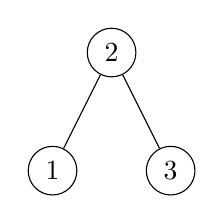
\begin{tikzpicture}[nodes={draw, circle}, -]
    \node{2}
    child { node {1} }
    child { node {3} };
    \end{tikzpicture}
    \caption{An undirected labelled graph with 3 nodes, $\mathcal{V}=\left\lbrace1,2,3\right\rbrace$ and $\mathcal{E}=\left\lbrace\left\lbrace1,2\right\rbrace\left\lbrace2,3\right\rbrace\right\rbrace$.}
    \label{fig:und_graph}
\end{figure} $\newline$
The \textit{neighbours} of node $i$ are defined as all nodes in $\mathcal{G}$ with an edge to node $i$,
\begin{equation*}
    \hbox{ne}\left(i\right)=\left\lbrace j\in\mathcal{V}:\left\lbrace i,j\right\rbrace\in\mathcal{E}\right\rbrace.
\end{equation*}
This definition can be extended to a set $A\subset\mathcal{V}$, where the neighbours of $A$ are defined as
\begin{equation*}
    \hbox{ne}\left(A\right)=\bigcup_{i\in A}\hbox{ne}\left(i\right)\setminus A.
\end{equation*}
A \textit{path} from $i_1$ to $i_m$ is defined as a sequence of certain nodes in $\mathcal{V}, i_1,i_2,...,i_m$, for which $\left(i_j,i_{j+1}\right)\in\mathcal{E}$ for $j=1,...,m-1$. Two nodes $i\notin C$ and $j\notin C$ are \textit{separated} by a subset $C\subset\mathcal{V}$, if every path from $i$ to $j$ contains at least one node from $C$. Two disjoint sets $A\subset\mathcal{V}\notin C$ and $B\subset\mathcal{V}\notin C$ are separated by $C$, if all $i\in A$ and $j\in B$ are separated by $C$, that is, it is not possible to "wander" on the graph from somewhere in $A$ and end somewhere in $B$ without crossing $C$.\\
If $i$ and $j$ are neighbours in $\mathcal{G}$, this can be expressed by $i\overset{\mathcal{G}}{\sim}j$ or $i\sim j$ for the case where the graph is implicit. It follows that $i\sim j\Longleftrightarrow j\sim i$. \\
Let $A$ be a subset of $\mathcal{V}$. A \textit{subgraph} $\mathcal{G}^A$ is a graph restricted to $A$, i.e., the graph obtained after removing all nodes that do not belong to $A$ and all edges where at least one node does not belong to $A$. $\mathcal{G}^A=\left\lbrace\mathcal{V}^A,\mathcal{E}^A\right\rbrace$, where $\mathcal{V}^A=A$ and 
\begin{equation*}
    \mathcal{E}^A = \left\lbrace\left\lbrace i,j\right\rbrace\in\mathcal{A} \hbox{ and } \left\lbrace i,j\right\rbrace\in A\times A\right\rbrace.
\end{equation*}
Let $\mathcal{G}$ be the graph in \autoref{fig:und_graph} and $\mathcal{A}=\left\lbrace2,3\right\rbrace$, then $\mathcal{V}^A=\left\lbrace2,3\right\rbrace$ and $\mathcal{E}^A=\left\lbrace\left\lbrace 2,3\right\rbrace\right\rbrace$ \autocite[][17--18]{rue2005gaussian}.
\subsection{Calculation of Summary Statistics}\label{sec:mean_iv}
As the posterior mean and the credibility intervals of coefficient are of interest, calculation of these is performed later on. This allows a better interpretation of the results. \\
To receive the expected value given a marginal function $\pi\left(x\right)$, the expected value of a function $f\left(x\right)$ is calculated, i.e.
\begin{equation}
    \int f\left(x\right)\pi\left(x\right)dx
\end{equation}
\autocite[][]{aitkin1991posterior}.\\
If necessary, e.g. if the target variable follows a (negative) binomial distribution, the value must be transformed to its original scale, as in these cases the log-likelihood is modelled. Therefore, in these cases, the expected value would have to be exponentiated to allow a clear interpretation. \\
In practice, to obtain the credibility interval of a variable, the marginal values are first transformed to their original scale, if necessary, and the 2.5\% quantile and the 97.5\% quantiles are calculated.
\clearpage
\section{Prior Selection}
A key question in Bayesian analysis is the effect of the prior on the posterior, and how that effect can be measured. Do posterior distributions derived with different priors become similar as more and more data is collected? It has been formally proven that under certain regularity conditions, the impact of the prior decreases with increasing sample size. From a practical point of view, it is more important to know what happens when the sample size $n$ is finite. In this section, different types of priors are introduced.
\subsection{Conjugate Priors}
One property of exponential families is that they have conjugate priors \autocite[][]{diaconis1979conjugate}, which is an important property in Bayesian statistics. If the posterior distribution $\pi\left(\pmb{\theta}|\pmb{y}\right)$ and the prior distribution $\pi\left(\pmb{\theta}\right)$ belong to the same probability distribution family, the prior and posterior distributions are called \textit{conjugate} distributions. Furthermore, the prior for the likelihood function $\pi\left(\pmb{y}|\pmb{\theta}\right)$ is called the \textit{conjugate prior}. These priors were first discussed and formalized by Raifa and Schlaifer in 1961 \autocite[][]{raiffaapplied}. \\
The construction of a conjugate prior is done by factorizing the likelihood function into two parts. One part must be independent of the parameter(s) of interest but can be dependent on the data, while the other factor is a function that depends on the parameter(s) of interest and is dependent on the data only through the sufficient statistics. The family of conjugate priors is by definition proportional to the second factor. The posterior distribution resulting from the conjugate prior is itself a member of the same family as the conjugate prior \autocite[][]{raiffaapplied}. In cases where the prior and posterior distributions are part of the same family, the prior is said to be closed under sampling. Furthermore, since the data are only incorporated into the posterior distribution through the sufficient statistics, there exist relatively simple formulas for updating the prior into the posterior.\\
For an example of the construction of a conjugated prior, see Fink 1997 \autocite[][]{fink1997compendium}.\\
A drawback of conjugated priors is that the a priori known information about $\mu$ may be insufficient for determining both parameters or may be inconsistent with the structure imposed by conjugacy \autocite[][]{robert2010bayesian}. Moreover, these priors can be too restrictive and not every belief about the prior can be described \autocite[][]{irwin2005prior}. \\
Thus, although conjugate priors are easy to handle both mathematically and computationally \autocite[][]{irwin2005prior}, they are not often used in practice because of these drawbacks.
\subsection{Penalized Complexity Priors}\label{sec:pc_prior}
One issue when selecting the prior distribution of a particular parameter is that it is not always intuitive when it comes to understanding and interpreting this distribution, something that is essential to ensure that it behaves as intended by the user. This problem can be addressed by using \textit{penalized complexity priors}, which is a methodology that penalizes the complexity of model components in relation to deviation from simple base model formulations.\\
PC priors provide a systematic and unified approach to calculating prior distributions for parameters of model components by using an inherited nested structure. This structure contains two models, the base model and a flexible version of the model. The first of the two is generally characterized by a fixed value of the relevant parameter, while the second version is considered a function of the random parameter. By penalizing the deviation from the flexible model to the fixed base model, the PC prior is calculated \autocite[][]{martins2014penalising}.
\subsubsection{The Principles Behind PC Priors}
Four main principles should be followed to calculate priors consistently and to understand their properties.
\subsubsection*{Support to Occam's Razor} 
Let $\pi\left(x|\xi\right)$ denote the density of a model component $x$ and $\xi$ the parameter to which a prior distribution is to be assigned. The base model is characterized by a density $\pi\left(x|\xi=\xi_0\right)$, where $\xi_0$ is a fixed value. The prior for $\xi$ should be such that proper shrinkage is given to $\xi_0$. The simplicity of the model is therefore prioritized over the complexity of the model, preventing overfitting \autocite[][]{martins2014penalising}.
\subsubsection*{Penalisation of Model Complexity} 
Let $f_1=\pi\left(x|\xi\right)$ and $f_0\left(x|\xi=\xi_0\right)$ denote the flexible model and the base model respectively. The complexity of $f_1$ compared to $f_0$ is characterized using the Kullback-Leibler divergence \autocite[][]{kullback1951information} to calculate a measure of complexity between the two models,
\begin{equation}
    \hbox{KLD}\left(f_1||f_2\right) = \int f_1\left(x\right)\log\left(\frac{f_1\left(x\right)}{f_0\left(x\right)}\right)dx.
\end{equation}
This can be used to measure the information that is lost when $f_1$ is approximated by the simpler model $f_0$. For multinormal densities with zero mean, the calculation simplifies to
\begin{equation}
    \hbox{KLD}\left(f_1||f_0\right) = \frac{1}{2}\left(\hbox{trace}\left(\pmb{\Sigma}_0^{-1}\pmb{\Sigma}_1\right)-n-\log\left(\frac{\left|\pmb{\Sigma}_1\right|}{\left|\pmb{\Sigma}_0\right|}\right)\right),
\end{equation}
where $f_i\sim\mathcal{N}\left(0,\pmb{\Sigma}_i\right), i=0,1$, while $n$ represents the dimension. For easier interpretation, the Kullback-Leibler divergence is transformed into a unidirectional distance measure
\begin{equation}
    d\left(\xi\right) = d\left(f_1||f_0\right)=\sqrt{2\hbox{KLD}\left(f_1||f_0\right)}
\end{equation}
which can be interpreted as a measure of distance from $f_1$ to $f_0$ \autocite[][]{martins2014penalising}.
\subsubsection*{Constant Rate Penalisation}
The derivation of the PC prior is based on a system of constant rate penalization, given by
\begin{equation}
    \frac{\pi_d\left(d\left(\xi\right)+\delta\right)}{\pi_d\left(d\left(\xi\right)\right)}=r^{\delta}, \hspace{20pt} d\left(\xi\right),\delta\geq0.
\end{equation}
$r\in\left(0,1\right)$ represents the constant decay rate and thus implies that the relative change in the prior distribution for $d\left(\xi\right)$ is independent of the actual distance. Therefore, $d\left(\xi\right)$ is exponentially distributed with density $\pi\left(d\left(\xi\right)\right)=\lambda\exp\left(-\lambda d\left(\xi\right)\right)$ and rate $\lambda = -\ln\left(r\right)$. By a standard variable change transformation, the corresponding PC prior for $\xi$ is given \autocite[][]{martins2014penalising}.
\subsubsection*{User-Defined Scaling}
Since $\lambda$ characterizes the shrinkage properties of the prior, it is important that the rate can be chosen in an intuitive and interpretable way. One possibility is to determine $\lambda$ by including a probability statement of tail events, for example
\begin{equation}\label{eq:pcprior}
    \mathbb{P}\left(Q\left(\xi\right) > U\right)=\alpha,
\end{equation}
where $U$ represents an assumed upper bound for an interpretable transformation $Q\left(\xi\right)$ and $\alpha$ denotes a small probability \autocite[][]{martins2014penalising}.
\subsubsection{Example: PC Prior for the Precision}
A PC prior can be used to adjust the smoothness of a spatial field in an intuitive way by specifying such a prior for the precision $\tau$. This makes it possible to adjust the smoothness of the spatial field in an intuitive way. In this case, the penalized complexity prior is defined by the parameter $\sigma_0$. Equation~\ref{eq:pcprior} therefore looks like this,
\begin{equation}\label{pcprec}
    \mathbb{P}\left(\sigma > \sigma_0\right)=\alpha.
\end{equation}
The actual expression of the prior is given by
\begin{equation}\label{eq:pc_prior_prec}
    \pi\left(\tau\right)=\frac{\lambda}{2}\tau^{-3/2}\exp\left(-\lambda\tau^{-1/2}\right),\hspace{20pt}\tau>0
\end{equation}
and is a type-2-Gumbel distribution. \\
The prior for $\tau$ corresponds to an exponential distribution with rate $\lambda$ for the standard deviation. \\
$\lambda$ quantifies the size of the penalty for deviation from the base model and is increased with higher values for it. \\
Here, $\lambda=\frac{-\log\left(\alpha\right)}{\sigma_0}$ \autocite[][]{martins2014penalising}.
\clearpage
\section{Markov-Chain-Monte-Carlo-Methods}
Markov chain Monte Carlo methods, also referred to as MCMC methods, are a set of algorithms that enable sampling from probability distributions based on the construction of Markov chains. After a sufficient number of iterations, the stationary distribution of a Markov chain can be taken as the desired distribution, with the quality of this distribution improving as the number of iterations increases. Most of the time, the construction of such a chain is relatively simple; the challenge is to determine how many steps are needed before convergence towards the stationary distribution is achieved. MCMC methods are mostly used to compute numerical approximations of multidimensional integrals, for instance in Bayesian statistics or computational biology. The two main concepts used in MCMC methods are Monte Carlo integration and the aforementioned Markov chains, hence the name Markov Chain Monte Carlo.
\subsection{Monte Carlo Integration}
\textit{Monte Carlo integration} is a technique that uses the generation of random numbers for numerical computation of definite integrals and is especially useful for higher-dimensional integrals. The problem the method addresses is the computation of the integral
\begin{equation}
    \mathbb{E}_f\left[h\left(X\right)\right]=\int_\chi h(x)f(x)dx.
\end{equation}
The integral can be approximated by using a sample $\left(X_1,...,X_m\right)$ generated from $f$ and calculating the arithmetic mean
\begin{equation}
    \overline{h}_m=\frac{1}{m}\sum_{j=1}^mh\left(x_j\right).
\end{equation}
According to the Strong Law of Large Numbers, $\overline{h}_m$ is likely to converge to $\mathbb{E}_f\left[h\left(X\right)\right]$. When the expectation of $h^2$ under $f$ is finite, the convergence speed of $\overline{h}_m$ can be assessed. The variance too can be estimated from the sample $\left(X_1,...,X_n\right)$ through
\begin{equation}
    v_m=\frac{1}{m^2}\sum_{j=1}^m\left[h\left(x_j\right)-\overline{h}_m\right]^2.
\end{equation}
For $m$ large,
\begin{equation}
    \frac{\overline{h}_m-\mathbb{E}_f\left[h\left(X\right)\right]}{\sqrt{v_m}}
\end{equation}
is approximately distributed as a $\mathcal{N}(0,1)$ variable. This can be used for constructing a convergence test and to calculate confidence bounds for the approximation of $\mathbb{E}_f\left[h\left(X\right)\right]$ \autocite[][83--84]{robert2013monte}. The term Monte Carlo was first used in 1949 by Metropolis and Ulam to describe a method dealing with problems related to "integro-differential equations that occur in various branches of the natural sciences" \autocite[][]{metropolis1949monte}.
\subsection{Markov Chains}
Markov chains are stochastic processes that aim to provide the probability of the occurrence of future events. A Markov chain is defined by the fact that even if only a limited history is known, predictions about future developments can be made just as reliably as if the entire history of a process were known. Thus, the probability of moving from the current state to any state depends only on the current state of the chain. These probabilities are defined by a \textit{transition kernel}, which is a function $K$ on $\mathcal{X} \times \mathcal{B}\left(\mathcal{X}\right)$, such that
\begin{itemize}
    \item[i.] $\forall x\in\mathcal{X}, K\left(x, \cdot\right)$ is a probability measure;
    \item[ii.] $\forall A\in \mathcal{B}\left(\mathcal{X}\right), K\left(\cdot, A\right)$ is measurable.
\end{itemize}
In the discrete case, the transition kernel is a matrix $\pmb{K}$ with elements
\begin{equation*}
    \mathbb{P}_{xy}=\mathbb{P}\left(X_n=y|X_{n-1}=x\right), \hspace{20pt}x,y\in\mathcal{X}.
\end{equation*}
If $\mathcal{X}$ is continuous, the kernel denotes the conditional density $K\left(x,x^T\right)$ of the transition $K\left(x,\cdot\right)$,
\begin{equation*}
    \mathbb{P}\left(X\in A|x\right)=\int_AK\left(x,x^T\right)dx^T.
\end{equation*}
Given a transition kernel $K$, a sequence $X_0,X_1,...,X_t$ of random variables is a \textit{Markov chain} $\left(X_n\right)$, if, for any $t$, the conditional distribution of $X_t$ given the previous states is the same as the distribution of $X_t$ given the last state, $x_{t-1}$,
\begin{align}
    \mathbb{P}\left(X_{t+1}\in A|x_0,x_1,x_2,...,x_t\right) &= \mathbb{P}\left(X_{t+1}\in A|x_t\right) \nonumber\\
    &= \int_A K\left(x_t, dx\right). 
\end{align}
These chains were first introduced by Markov in 1906 \autocite[][]{markov1906extension}. Markov chains can have certain properties that affect their long-term behaviour and are of particular importance for MCMC algorithms. In Sections~\ref{sssec:irreducibility}--~\ref{sssec:stationary}, some of them are introduced.
\subsubsection{Irreducibility} \label{sssec:irreducibility}
Irreducibility is critical to the construction of Markov chain Monte Carlo algorithms, as it ensures the convergence of such an algorithm. A Markov chain is \textit{irreducible} if all states communicate, that is, for all states $i$ and $j$ the probability of going from $i$ to $j$ in finite time is true positive. \\
Formally speaking, given a measure $\varphi$, a Markov chain $\left(X_n\right)$ with transition kernel $K\left(x,y\right)$ is $\varphi$-\textit{irreducible}, if, for every $A\in B\left(\mathcal{X}\right)$ with $\varphi\left(A\right)>0$, there exists $n$ such that $K^n\left(x,A\right) \forall x\in\mathcal{X}$. The chain is \textit{strongly} $\varphi$-\textit{irreducible} if $n=1\forall$ measurable $A$ \autocite[][213--214]{robert2013monte}.
\subsubsection{Periodicity} 
The behaviour of a Markov chain can sometimes be limited by deterministic constraints on the transitions from $X_n$ to $X_{n+1}$. For discrete chains, the \textit{period} of a state $w\in\mathcal{X}$ is defined as. 
\begin{equation*}
    d\left(w\right)=\hbox{g.c.d. } \lbrace m\geq 1;K^m\left(w,w\right)>0\rbrace,
\end{equation*}
with g.c.d the greatest common denominator. If a Markov chain is irreducible, the transition matrix can be written as a block matrix
\begin{equation}
    \pmb{P}=\begin{pmatrix}
    0 & \pmb{D}_1 & 0 & \dots & 0\\
    0 & 0 & \pmb{D}_2 & \dots & 0 \\
    \vdots & \vdots & \ddots  \\
    \pmb{D}_d & 0 & 0 & & 0
    \end{pmatrix},
\end{equation}
It is evident that at every $d$-th step there is a return to the initial group. There exists only one value for the period when a chain is irreducible. If this value is 1, the irreducible chain is \textit{aperiodic} \autocite[][217--218]{robert2013monte}.
\subsubsection{Transience and Recurrence} 
To guarantee an acceptable approximation of a simulated model, a Markov chain needs to have good stability properties. Irreducibility is not strong enough to ensure that the trajectory of $\left(X_n\right)$ enters $A$ often enough. This leads to the formalization of \textit{recurrence} and \textit{transience}.  \\
In a finite space $\mathcal{X}$, a state $w\in\mathcal{X}$ is \textit{transient} if it is finitely often visited and \textit{recurrent} if it is almost certainly infinitely often visited. \\
For irreducible chains, these two properties are properties of the chain, not of a particular state \autocite[][218--219]{robert2013monte}.
\subsubsection{Ergodicity}
When looking at a Markov chain $\left(X_n\right)$ from a temporal point of view, it is essential to establish to what the chain is converging. A natural candidate for the limiting distribution is the stationary distribution $\pi$ which leads to the need to define sufficient conditions on $\left(X_n\right)$ for $X_n$ to be asymptotically distributed according to $\pi$. There are several conditions that can be imposed on the convergence of $P^n$, the distribution of $X_n$ to $\pi$. The most fundamental and important is that of \textit{ergodicity}, that is, independence of initial conditions.\\
If a Markov chain $\left(X_n\right)$ is both aperiodic and positive recurrent, it is called an \textit{ergodic} Markov chain \autocite[][231--234]{robert2013monte}.
\subsubsection{Stationary distribution} \label{sssec:stationary}
A chain $\left(X_n\right)$ is more stable if the marginal distribution of $X_n$ is independent of $n$. This is a requirement for the existence of a probability distribution $\pi$ such that $X_{n+1}\sim\pi$ if $X_n\sim\pi$. Markov chain Monte Carlo methods rely on the fact that this condition can be satisfied. \\
A $\sigma$-finite measure $\pi$ is \textit{invariant} for the transition kernel $K\left(\cdot,\cdot\right)$ if \begin{equation*}
    \pi\left(B\right)=\int_\mathcal{X}K\left(x,B\right)\pi(dx), \hspace{20pt} \forall B\in\mathcal{B}\left(\mathcal{X}\right).
\end{equation*}
This distribution is referred to as \textit{stationary} if $\pi$ is a probability measure, as $X_0\sim\pi$ implies that $X_n\sim\pi$ is $\forall n$. An irreducible Markov chain has a stationary distribution precisely if it is positively recurrent. The distribution is given by
\begin{equation}
    \pi_x=\left(\mathbb{E}_x\left[\tau_x\right]\right)^{-1}, \hspace{20pt} x\in\mathcal{X},
\end{equation}
where $\mathbb{E}_x\left[\tau_x\right]$ can be interpreted as the average number of transitions between two passages in $x$. \\
In practice, the stationary distributions are often of special interest. If these distributions are defined as the starting distribution of $X_0$, all following distributions of the states $X_n$ for any $n$ are equal to the starting distribution. The interesting question here is when such distributions exist and when any distribution converges against a stationary distribution of this kind \autocite[][223--224]{robert2013monte}.
\subsection{The Metropolis-Hastings Algorithm}
Having established the basics of MCMC methods, one of the best known MCMC algorithms, the Metropolis-Hastings algorithm, is introduced next. The algorithm is based on the Metropolis algorithm, which was developed to simulate the states of a system according to the Boltzmann distribution, with the newest state always depending on the previous state \autocite[][]{metropolis1953equation}. \\ 
The Metropolis-Hastings algorithm is a procedure for drawing random samples from a probability distribution from which direct sampling is difficult if a function proportional to the \textit{target density} $f$ is known.
This function $q\left(\pmb{y}|\pmb{x}\right)$ is called the \textit{proposal density} and must be easy to simulate in order for the Metropolis-Hastings algorithm to be implementable. Moreover, it must be either explicitly present or \textit{symmetric}, meaning $q\left(\pmb{x}|\pmb{y}\right)=q\left(\pmb{y}|\pmb{x}\right)$. \\
The Metropolis-Hastings algorithm of a target density $f$ and proposal density $q$ produces a Markov chain $\left(X^{(t)}\right)$ by the following transition.
\begin{algorithm}[H]
\caption{The Metropolis-Hastings Algorithm}
\begin{algorithmic}[1]
\Statex Given $f\left(\pmb{x}\right)$ and $q\left(\pmb{y}|\pmb{x}\right)$
\State Initialization: Choose arbitrary $x_t$ as the first sample
\For{each iteration $t$}
    \State Generate $Y_t\sim q\left(\pmb{y}|x^{(t)}\right)$
    \State Take 
    \begin{align}
        X^{(t+1)}&=\begin{cases}
        Y_t & \hbox{with probability } \mathbb{P}\left(x^{(t)}, Y_t\right) \\
        x^{(t)} & \hbox{with probability } 1-\mathbb{P}\left(x^{(t)}, Y_t\right)
        \end{cases} \nonumber \\
    \hbox{where} \nonumber\\
    \mathbb{P}\left(x,y\right) &= \min\left\lbrace\frac{f\left(\pmb{y}\right)}{f\left(\pmb{x}\right)}\frac{q\left(\pmb{x}|\pmb{y}\right)}{q\left(\pmb{y}|\pmb{x}\right)}, 1\right\rbrace.
    \end{align} 
    \EndFor
\end{algorithmic}
\end{algorithm}  $\newline$
$\mathbb{P}\left(x,y\right)$ is the \textit{Metropolis-Hastings acceptance probability}. \\
The algorithm always accepts values $y_t$ that lead to an increase in the ratio $f\left(y_t\right)/q\left(y_t|x^{(t)}\right)$ compared to the previous value $f\left(x^{(t)}\right)/q\left(x^{(t)}|y_t\right)$. In the symmetric case, the acceptance probability simplifies to
\begin{equation*}
     \mathbb{P}\left(x,y\right) = \min\left\lbrace\frac{f\left(\pmb{y}\right)}{f\left(\pmb{x}\right)}, 1\right\rbrace
\end{equation*}
\autocite[][]{hastings1970monte}. \\
If the Markov chain starts with a value $x^{(0)} > 0$, then $f\left(x^{(t)}\right) > 0\,\,\forall t\in\mathbb{N}$ since the values of $y$ such that $f\left(y_t\right) = 0$ are all rejected by the algorithm. As the number of iterations $t$ increases, the distribution of saved states $x_0,...,x_t$ converges towards the target density $f(\pmb{x})$ \autocite[][270--275]{robert2013monte}.
\clearpage
\section{Latent Gaussian Models and INLA}
In recent years, a growing amount of georeferenced data has become available, leading to an increased need for appropriate statistical modelling to handle large and complex datasets. The usual approach to inference for latent Gaussian models involves the previously introduced Markov chain Monte Carlo methods. Due to several factors, these methods may perform poorly when applied to such models. One factor is the interdependence of the components of the latent field $\pmb{x}$ while another is that $\pmb{\theta}$ and $\pmb{x}$ are highly dependent on each other, especially for large $n$. The first of these problems can potentially be overcome by constructing a joint proposal based on a Gaussian approximation of the full conditional of $\pmb{x}$ \autocite[][]{gamerman1997sampling}, while the second problem requires, at least in part, a joint update of $\pmb{\theta}$ and $\pmb{x}$. There are several proposals to solve these shortcomings, but MCMC sampling continues to show poor computational speed \autocite[][322]{rue2009approximate}.\\
Bayesian hierarchical models have proven to be effective in capturing complex stochastic structures in spatial processes. A large proportion of these models are based on latent Gaussian models, a subclass of structured additive regression models. These models include Integrated Nested Laplace Approximations (INLA), which are a class of models used to approximate the posterior marginals of a latent Gaussian field. These approximations work by reformulating the regression model as a three-part hierarchical model. The parts are as follows:
\begin{itemize}
    \item[1.] Approximation of the posterior marginal of $\pmb{\theta}$ by using the Laplace approximation.
    \item[2.] Computation of the (simplified) Laplace approximation for selected values of $\pmb{\theta}$ to improve the Gaussian approximation.
    \item[3.] Combination of the first two parts by numerical integration.
\end{itemize}
$\pmb{\theta}$ is a vector of hyperparameters. The hyperparameters $\pmb{\theta}$ can be, for example, the variance in the Gaussian likelihood or the shape parameter in the likelihood of the gamma distribution. In the case of latent fields, they can be, for instance, dispersion parameters or spatial correlation parameters \autocite[][]{rue2009approximate}.
\subsection{Notation and Basic Properties}
\label{sec:notation}
For structured additive regression models, the distribution of the response variable $y_i$ is assumed to be a member of the exponential family, with the mean $\mu_i$ linked to a structured additive predictor $\eta_i$ by a link function $g\left(\cdot\right)$ such that $g\left(\mu_i\right)=\eta_i$. The predictor $\eta_i$  takes into account the effect of multiple covariates in an additive way,
\begin{equation}\label{eq:predictor}
    \eta_i=\alpha+\sum_{j=1}^{n_f}f^{(j)}\left(u_{ji}\right)+\sum_{k=1}^{n_{\beta}}\beta_kz_{ki}+\epsilon_i, \hspace{20pt}i=1,...,n
\end{equation}
\autocite[][]{stone1985additive}.\\
The $\left\lbrace f^{(j)}\left(\cdot\right)\right\rbrace$s are unknown functions of the covariates $u$, while the $\left\lbrace\beta_k\right\rbrace$s represent the linear effect of the covariates $z$ and the $\epsilon_i$s are unstructured terms. Latent Gaussian models assign a Gaussian prior to $\alpha$, $\left\lbrace f^{(j)}\left(\cdot\right)\right\rbrace$ and $\left\lbrace\epsilon_i\right\rbrace$. In the following $\pmb{x}$ shall denote the vector of all latent Gaussian variables ($\left\lbrace\eta_i\right\rbrace$, $\alpha$, $\left\lbrace f^{(j)}\right\rbrace$ and $\left\lbrace\beta_k\right\rbrace$) and $\pmb{\theta}$ the vector of hyperparameters.\\
The conditional density $\pi\left(\pmb{x}|\theta_1\right)$ is Gaussian with an assumed zero mean and precision matrix $\pmb{Q}\left(\theta_1\right)$. The Gaussian density $\mathcal{N}\left(\mu,\pmb{\Sigma}\right)$ with mean $\mu$ and covariance $\pmb{\Sigma}$ at configuration $\pmb{x}$ is denoted by $\mathcal{N}\left(\pmb{x};\mu,\pmb{\Sigma}\right)$. For simplicity, $\left\lbrace\eta_i\right\rbrace$ is included instead of $\left\lbrace\epsilon_i\right\rbrace$. \\
The distribution for the $n_d$ observational variables $y=\left\lbrace y_i:i\in\mathcal{I}\right\rbrace$ is denoted by $\pi\left(\pmb{y}|\pmb{x}, \theta_2\right)$ and is assumed conditionally independent given $\pmb{x}$ and $\theta_2$. Let $\pmb{\theta}=\left(\theta_1^T,\theta_2^T\right)^T$ with $\dim\left(\pmb{\theta}\right)=m$. For non-singular $\pmb{Q}\left(\pmb{\theta}\right)$ the posterior is given by
\begin{align}
    \pi\left(\pmb{x},\pmb{\theta}|\pmb{y}\right)&\propto\pi\left(\pmb{\theta}\right)\pi\left(\pmb{x}|\pmb{\theta}\right)\prod_{i\in I}\pi\left(y_i|x_i,\pmb{\theta}\right) \nonumber\\
    &\propto \pi\left(\pmb{\theta}\right)\left|\pmb{Q}\left(\pmb{\theta}\right)\right|^{1/2}\exp\left[-\frac{1}{2}\pmb{x}^T\pmb{Q}\left(\pmb{\theta}\right)\pmb{x}+\sum_{i\in I}\log\left\lbrace\pi\left(y_i|x_i,\pmb{\theta}\right)\right\rbrace\right].
\end{align}
Most latent Gaussian models satisfy two basic properties:
\begin{itemize}
    \item[1.] The latent field $\pmb{x}$ is of large dimension, $n\approx10^2-10^5$. Therefore, the latent field is a Gaussian Markov random field with sparse precision matrix $\pmb{Q}\left(\pmb{\theta}\right)$.
    \item[2.] The number of hyperparameters, $m$, is small, $m\leq6$.
\end{itemize}
In most cases, both properties are required to produce fast inference, and thus these are assumed to be true for the remainder of this work \autocite[][]{rue2009approximate}.
\subsection{Applications for Latent Gaussian Models}
Latent Gaussian models can be employed in a vast range of different domains, in fact most structured Bayesian models are of this particular form. Some of these domains are presented below.
\subsubsection{Regression Models}
Bayesian generalized linear models correspond to the linear relationship $\eta_i=\alpha+\sum_{k=1}^{n_\beta}\beta_k z_{ki}$ \autocite[][]{dey2000generalized}. Either the linear relationship of the covariates can be relaxed through the $f\left(\cdot\right)$ terms \autocite[][]{fahrmeir2013multivariate}, random effects can be introduced through them or both. Smooth covariate effects are frequently modelled using penalized spline models \autocite[][]{lang2004bayesian} or random walk models \autocite[][]{fahrmeir2013multivariate}, continuous indexed spline models \autocite[][]{rue2005gaussian} or Gaussian processes \autocite[][]{chu2005gaussian}. The incorporation of random effects allows for the consideration of overdispersion caused by unobserved heterogeneity or correlation in longitudinal data and can be introduced by defining $f\left(u_i\right)=f_i$ and $\left\lbrace f_1\right\rbrace$ to be independent, zero mean and Gaussian \autocite[][]{fahrmeir2001bayesian}.
\subsubsection{Dynamic Models}
Temporal dependence can be introduced by using $i$ in \eqref{eq:predictor} as temporal index $t$ and defining $f\left(\cdot\right)$ and $\pmb{u}$ such that $f\left(u_t\right)=f_t$. Both a discrete-time and a continuous-time autoregressive model can be modelled by $\left\lbrace f_t\right\rbrace$. Furthermore, a seasonal effect or the latent process of a structured time series model can be modelled \autocite[][]{kitagawa1996smoothness}. Alternatively, a smooth temporal function in the same sense as for regression models can be represented by $\left\lbrace f_t\right\rbrace$.
\subsubsection{Spatial and Spatio-Temporal Models}
Similar to the previous type of model, spatial dependence can be modelled by a spatial covariate $\pmb{u}$ such that $f\left(u_s\right)=f_s$, where $s$ denotes the spatial location or region $s$. The stochastic model for $f_s$ is constructed to promote spacial smooth realizations of some sort. Popular models of this type include the Besag-York-Mollié \autocite[][]{besag1991bayesian} model with extensions for regional data, continuous indexed Gaussian models \autocite[][]{banerjee2014hierarchical} and texture models \autocite[][]{marroquin2001gauss}. The dependence between spatial and temporal covariates can be achieved either by using a spatio-temporal covariate $(s,t)$ or a corresponding spatio-temporal Gaussian field \autocite[][]{kammann2003geoadditive}.\\
Often the final model consists of a sum of several components, e.g. a spatial component, random effects and both linear and smooth effects of some covariates. In order to separate the effects of the different components in \eqref{eq:predictor}, sometimes linear or sum-to-zero constraints can be imposed \autocite[][319--321]{rue2009approximate}.
\subsection{Gaussian Random Fields}
Let $\pmb{s} = \left(s_1,...,s_n\right)^T$ be a vector of locations. A \textit{Gaussian random field} (GRF)
\begin{equation}
    \left\lbrace Z(s):s\in D\subset\mathbb{R}^2\right\rbrace
\end{equation}
is a set of random variables where the observations occur in a continuous domain and where each finite set of random variables follows a multivariate normal distribution. A random process $Z\left(\cdot\right)$ is strictly stationary if it is invariant to shifts, i.e., if for each set of locations and each $h\in\mathbb{R}^2$ the distribution of $\pmb{Z(s)}=\left(Z\left(s_1\right),... ,Z\left(s_n\right)\right)$ is equal to that of $\pmb{Z(s+h)}=\left(Z\left(s_1+h\right),...,Z\left(s_n+h\right)\right)$. A less constraining requirement is given by second-order stationarity. Under this condition, the process has a constant mean value
\begin{equation}
    \mathbb{E}\left[\pmb{Z(s)}\right] = \mu, \hspace{20pt}\forall s\in D,
\end{equation}
and the covariances depend only on the differences between locations
\begin{equation}
    \hbox{Cov}\left(\pmb{Z(s)}, \pmb{Z(s+h)}\right)=C\left(\pmb{h}\right), \hspace{20pt}\forall \pmb{s}\in D,\,\forall \pmb{h}\in\mathbb{R}^2.
\end{equation}
Furthermore, if the covariances depend only on the distances between the locations and not on the directions, the process is called isotropic. Else, the process is anisotropic. An intrinsically stationary process has a constant mean value and satisfies
\begin{equation}
    \hbox{Var}\left(Z\left(s_i\right)-Z\left(s_j\right)\right)=2\gamma\left(s_i-s_j\right),\hspace{20pt}\forall s_i,s_j.
\end{equation}
$2\gamma\left(\cdot\right)$ is the variogram and $\gamma\left(\cdot\right)$ is called the semivariogram \autocite[][]{cressie2015statistics}. Under the assumption of intrinsic stationarity, the constant-mean assumption implies
\begin{equation*}
    2\gamma\left(\pmb{h}\right)=\hbox{Var}\left(\pmb{Z(s+h)}-\pmb{Z(s)}\right)=\mathbb{E}\left[\left(\pmb{Z(s+h)}-\pmb{Z(s)}\right)^2\right],
\end{equation*}
and the estimation of the semivariogram can be obtained using the empirical semivariogram as follows:
\begin{equation}
    2\widehat{\gamma}\left(\pmb{h}\right)=\frac{1}{\left|N\left(\pmb{h}\right)\right|}\sum_{N\left(\pmb{h}\right)}\left(Z\left(s_i\right)-Z\left(s_j\right)\right)^2,
\end{equation}
where $N\left(\pmb{h}\right)=\left\lbrace\left(s_1,s_j\right):s_i-s_j=\pmb{h}, i,j=1,...,n\right\rbrace$ denotes the number of pairs and $\left|N\left(\pmb{h}\right)\right|$ the number of distinct pairs. For isotropic processes, the semivariogram is a function of distance $h=\left|\left|\pmb{h}\right|\right|$.   \\
Plotting the empirical semivariogram against the separation distance conveys essential information regarding the continuity and spatial variability of the process. Given relatively short distances, the semivariogram tends to be small but increases with distance, indicating the similarity of observations in proximity. The semivariogram levels off to a nearly constant value, also called the sill, as the separation distance increases, indicating a decrease in spatial dependence with distance within the range and no spatial correlation outside the range, which is reflected in a nearly constant variance. If there is a discontinuity or a vertical jump at the origin, the process has a nugget effect, which is often due to a measurement error, but may be indicative of a spatially discontinuous process.
\begin{figure}
    \centering
    \includegraphics[width=\textwidth]{typicalsemivariogram-1.png}
    \caption{A typical semivariogram}
    \label{fig:semivariogram}
\end{figure}
The empirical semivariogram is an exploratory tool useful for assessing whether data exhibit spatial correlation. Furthermore, it can be compared to a Monte Carlo envelope of empirical semivariograms calculated from random permutations of the data while keeping the locations fixed \autocite[][]{diggle2003introduction}. If the empirical semivariogram lies outside the Monte Carlo envelope with increasing distance, this is an indication of spatial correlation.\\
An example of a semivariogram is shown in Figure~\ref{fig:semivariogram}. This graph is taken from "Geospatial Health Data: Modelling and Visualization with R-INLA and Shiny" by Paula Moraga \autocite[][]{moraga2019geospatial}. 
% \\ 
% The dependence structure of a GRF is given by the covariance matrix, which is constructed from a covariance function. Matérn models and exponential functions are conventionally used for this purpose \autocite[][]{gelfand2010handbook}. For the locations $s_i, s_j\in\mathbb{R}^2$ the exponential covariance function is given by
% \begin{equation}
% \hbox{Cov}\left(Z\left(s_i\right), Z\left(s_j\right)\right)=\sigma^2\exp\left(-\kappa\left|\left|s_i-s_j\right|\right|\right),
% \end{equation}
% where the distance between the locations $s_i$ and $s_j$ is denoted by $\left|\left|s_i-s_j\right|\right|$, the variance of the spatial field is given by $\sigma^2$, while $\kappa>0$ controls the rate at which the correlation decays as the distance increases. \\
% The Matérn family represents a flexible class of covariance functions that arises naturally in a variety of scientific fields \autocite[][]{guttorp2006studies}. The Matérn covariance function is written as
% \begin{equation}
%     \hbox{Cov}\left(Z\left(s_i\right),Z\left(s_j\right)\right)=\frac{\sigma^2}{2^{\nu-1}\Gamma\left(\nu\right)}\left(\kappa\left|\left|s_i-s_j\right|\right|\right)^{\nu}K_\nu\left(\kappa\left|\left|s_i-s_j\right|\right|\right).
% \end{equation}
% $\sigma^2$ denotes the marginal variance of the spatial field, $K_\nu\left(\cdot\right)$ represents the modified Bessel function of second kind and order $\nu>0$, where $\nu$ is an integer. The mean square differentiability of the process is determined by $\nu$ and is usually fixed since it is difficult to identify in applications. For $\nu=0.5$, this covariance function is the equivalent of the exponential covariance function. $\kappa > 0$ is related to the range $\rho$, which is defined as the distance at which there is approximately no correlation between two given points, $\rho=\sqrt{8\nu}/\kappa$ to be exact \autocite[][]{cameletti2013spatio}. Examples of these two covariance functions are shown in Figure~\ref{fig:covariance}. These graphs are again taken from "Geospatial Health Data: Modeling and Visualization with R-INLA and Shiny" by Paula Moraga \autocite[][]{moraga2019geospatial}. 
% \begin{figure}[H]
%     \centering
%     \includegraphics[width=0.8\textwidth]{covariancefunctions-1.png}
%     \includegraphics[width=0.8\textwidth]{covariancefunctions-2.png}
%     \caption{Covariance functions corresponding to exponential and Matérn models.}
%     \label{fig:covariance}
% \end{figure}
\subsection{Gaussian Markov Random Fields}
\subsubsection{Definition of GMRFs}
Let $\pmb{x}=\left(x_1,...,x_n\right)^T$ be normally distributed with mean $\pmb{\mu}$ and covariance matrix $\pmb{\Sigma}$. Let $\mathcal{G}=\left(\mathcal{V}, \mathcal{E}\right)$, where $\mathcal{V}=\left\lbrace 1,...,\right\rbrace$ and $\mathcal{E}$ be such that there is no edge between nodes $i$ and $j$ exactly when $x_i\perp x_j|\pmb{x}_{ij}$. Then $\pmb{x}$ is a \textit{Gaussian Markov random field} (GMRF) with respect to $\mathcal{G}$. \\
Since $\pmb{\mu}$ does not affect the pairwise conditional independence properties of $\pmb{x}$, this information is 'hidden' in $\pmb{\Sigma}$. Hence,
\begin{equation*}
    x_i\perp x_j|x_{ij}\Longleftrightarrow Q_{ij}=0.
\end{equation*}
Therefore, the non-zero pattern of $\pmb{Q}$ determines $\mathcal{G}$, i.e. whether $x_i$ and $x_j$ are conditionally independent, and can be derived from $\pmb{Q}$. If $\pmb{Q}$ is a fully dense matrix, $\mathcal{G}$ is fully connected, implying that any normal distribution with SPD covariance matrix is a GMRF and vice versa. \\
The elements of $\pmb{Q}$ are used for conditional interpretations. For any GMRF with respect to $\mathcal{G}=\left(\mathcal{V}, \mathcal{E}\right)$ with mean $\pmb{\mu}$ and precision matrix $\pmb{Q} > 0$,
\begin{align}
    \mathbb{E}\left[x_i|\pmb{x}_{-i}\right] &= \mu_i-\frac{1}{Q_{ii}}\sum_{j:j\sim i}Q_{ij}\left(x_j-\mu_j\right), \label{eq:mean_gmrf}\\
    \hbox{Prec}\left(x_i|\pmb{x}_{-i}\right) &= Q_{ii} \hspace{20pt}\hbox{ and }\label{eq:prec_gmrf}\\
    \hbox{Corr}\left(x_i,x_j|\pmb{x}_{ij}\right) &= -\frac{Q_{ij}}{\sqrt{Q_{ii}Q_{jj}}},\hspace{20pt} i\neq j
\end{align}
\autocite[][21]{rue2005gaussian}. \\
On the main diagonal of $\pmb{Q}$ are the conditional precisions of $x_i$ given $\pmb{x}_{-i}$ are placed, while the other elements, when scaled appropriately, provide information about the conditional correlation between $x_i$ and $x_j$ given $\pmb{x}_{ij}$. Since $\hbox{Var}\left(x_i\right)=\Sigma_{ii}$ and $\hbox{Corr}\left(x_i,x_j\right)=\Sigma_{ij}/\sqrt{\Sigma_{ii}\Sigma_{jj}}$, the information about the marginal variance of $x_i$ and the marginal correlation between $x_i$ and $x_j$ is given by $\pmb{\Sigma}$. The marginal interpretation provided by the correlation matrix is intuitive and informative, as the scope of the interpretation is reduced from a $n$-dimensional distribution to a one- or two-dimensional distribution. $\pmb{Q}$ is difficult to interpret marginally because either $\pmb{x}_{-i}$ or $\pmb{x}_{ij}$ would have to be integrated out of the joint distribution parameterized with respect to $\pmb{Q}$. $\pmb{Q}^{-1}=\pmb{\Sigma}$ by definition, and in general $\Sigma_{ii}$ depends on each element in $\pmb{Q}$ and vice versa \autocite[][20--23]{rue2005gaussian}.
\subsubsection{Markov Properties of GMRFs}
One property of GMRFs is that more information regarding conditional independence can be extracted from $\mathcal{G}$. The following three properties are equivalent. \\
The \textit{pairwise Markov property}:
\begin{equation*}
    x_i\perp x_j|\pmb{x}_{ij}\hspace{20pt}\hbox{ if }\left\lbrace i,j\right\rbrace\notin\mathcal{E}\hbox{ and }i\neq j.
\end{equation*}
The \textit{local Markov property}:
\begin{equation*}
    x_i\perp \pmb{x}_{-\left\lbrace i, \hbox{ne}\left(i\right)\right\rbrace}|\pmb{x}_{\hbox{ne}\left(i\right)}\hspace{20pt}\forall i\in\mathcal{V}.
\end{equation*}
The \textit{global Markov property}:
\begin{equation*}
    \pmb{x}_{A}\perp \pmb{x}_{B}|\pmb{x}_{C}
\end{equation*}
for all disjoint sets $A$, $B$ and $C$ where $A$ and $B$ are non-empty and separated by $C$. \\ Illustrations for these properties are shown in Figure~\ref{fig:pairwise}, Figure~\ref{fig:local} and Figure~\ref{fig:global}. These illustrations are taken from Rue and Held \autocite[][23--24]{rue2005gaussian}.
\begin{figure}[H]
    \centering
    \ctikzfig{ind_fig1}
    \caption{The pairwise Markov property; the black nodes are conditionally independent given the light grey nodes.}
    \label{fig:pairwise}
\end{figure}
\begin{figure}[H]
    \centering
    \ctikzfig{ind_fig2}
    \caption{The local Markov property; the black nodes and white nodes are conditionally independent given the dark grey nodes.}
    \label{fig:local}
\end{figure}
\begin{figure}[H]
    \centering
    \ctikzfig{ind_fig3}
    \caption{The global Markov property; the dark grey and light grey nodes are globally independent given the black nodes.}
    \label{fig:global}
\end{figure}
\subsubsection{Conditional Properties of GMRFs}
An essential result of GMRFs is the conditional distribution for a subset $\pmb{x}_a$ given $\pmb{x}_{-A}$. Here the canonical parameterization proves useful, since by definition it can be easily updated by successive conditioning. \\
By splitting the indices into the non-empty sets A and B, of which the latter is equal to -A,
\begin{equation}\label{eq:partition_1}
    \pmb{x}=\begin{pmatrix}\pmb{x}_A\\\pmb{x}_B\end{pmatrix}.
\end{equation}
The mean and the precision are divided accordingly,
\begin{equation}\label{eq:partition_2}
    \pmb{\mu}=\begin{pmatrix}\pmb{\mu}_A\\\pmb{\mu}_B\end{pmatrix},\hspace{20pt}\hbox{ and }\hspace{20pt}\pmb{Q}=\begin{pmatrix}\pmb{Q}_{AA} & \pmb{Q}_{AB} \\ \pmb{Q}_{BA} & \pmb{Q}_{BB}\end{pmatrix}.
\end{equation}
The conditional distribution of $\pmb{x}_A|\pmb{x}_B$ is a GMRF with respect to the subgraph $\mathcal{G}^A$ with mean $\pmb{\mu}_{A|B}$ and precision matrix $\pmb{Q}_{A|B}>0$, where
\begin{equation}
    \pmb{\mu}_{A|B}=\pmb{\mu}_A-\pmb{Q}_{AA}^{-1}\pmb{Q}_{AB}\left(\pmb{x}_B-\pmb{\mu}_B\right)
\end{equation}
and
\begin{equation*}
    \pmb{Q}_{A|B}=\pmb{Q}_{AA}.
\end{equation*}
Thus, the explicit knowledge of $\pmb{Q}_{A|B}$ is available through $\pmb{Q}_{AA}$, i.e. no calculation is required to obtain the conditional precision matrix. Moreover, the conditional mean depends only on the values of $\pmb{\mu}$ and $\pmb{Q}$ in $A\cup\,\hbox{ne}\left(A\right)$, since $Q_{ij} = 0\,\forall j\not in\hbox{ne}\left(i\right)$. \\
For successive conditioning, the canonical parameterization for GMRF is useful. \\
A GMRF $\pmb{x}$ with respect to $\mathcal{G}$ and canonical parameters $\pmb{b}$ and $\pmb{Q}>0$ has the density
\begin{equation*}
    \pi\left(\pmb{x}\right)\propto\exp\left(-1\frac{1}{2}\pmb{x}^T\pmb{Q}\pmb{x}+\pmb{b}^T\pmb{x}\right).
\end{equation*}
The precision matrix is $\pmb{Q}$ and the mean is $\pmb{\mu}=\pmb{Q}^{-1}\pmb{b}$. The canonical parameterization is written as 
\begin{equation*}
    \pmb{x}\sim \mathcal{N}_C\left(\pmb{b},\pmb{Q}\right).
\end{equation*}
Furthermore,
\begin{equation*}
    \mathcal{N}\left(\pmb{\mu},\pmb{Q}^{-1}\right) \Longleftrightarrow \mathcal{N}_C\left(\pmb{Q\mu}, \pmb{Q}\right).
\end{equation*}
If the indices are partitioned into two non-empty sets A and B and $\pmb{x}$, $\pmb{b}$ and $\pmb{Q}$ are partitioned as in \eqref{eq:partition_1} and \eqref{eq:partition_2}, then
\begin{equation}
    \pmb{x}_A|\pmb{x}_B\sim\mathcal{N}_C\left(\pmb{b}_A-\pmb{Q}_{AB}\pmb{x}_B,\pmb{Q}_{AA}\right).
\end{equation}
Let $\pmb{y}|\pmb{x}\sim\mathcal{N}\left(\pmb{x},\pmb{P}^{-1}\right)$ and $\pmb{x}\sim\mathcal{N}_C\left(\pmb{b},\pmb{Q}\right)$, then
\begin{equation}
    \pmb{x}|\pmb{y}\sim\mathcal{N}_C\left(\pmb{b}+\pmb{Py}, \pmb{Q}+\pmb{P}\right).
\end{equation}
This allows the calculation of conditional densities with multiple sources of conditioning, e.g. conditioning on observed data and a subset of variables. Therefore, the canonical parameterization can be repeatedly updated without explicitly calculating the mean until it is needed. The computation of the mean requires the solution of $\pmb{Q\mu}=\pmb{b}$, but only matrix-vector products are needed for updating the canonical parameterization \autocite[][25--27]{rue2005gaussian}.
\subsubsection{Specification Through Full Conditionals}
Alternatively, a GMRF can be specified by the full conditionals $\left\lbrace\pi\left(x_i|\pmb{x}_{-i}\right)\right\rbrace$ in place of $\pmb{\mu}$ and $\pmb{Q}$. Suppose the full conditionals are given as normals with
\begin{align}
    \mathbb{E}\left[x_i|\pmb{x}_{-i}\right] &= \mu_i-\sum_{j:j\sim i}\beta_{ij}\left(x_j-\mu_j\right)\hspace{20pt}\hbox{ and}\\
    \hbox{Prec}\left(x_i|\pmb{x}_{-i}\right) &= \kappa_i>0
\end{align}
for $i=1,...,n$, for $\pmb{\mu}$, $\pmb{\kappa}$ and some $\left\lbrace\eta_{ij},i\neq j\right\rbrace$. Evidently, $\sim$ is implicitly defined by the non-zero terms of $\left\lbrace\beta_{ij}\right\rbrace$. For there to exist a joint density $\pi\left(\pmb{x}\right)$ leading to these full conditional distributions, these full conditionals must be consistent. Since $\sim$ is symmetric, it follows that if $\beta_{ij}\neq 0$, then $\beta_{ji}\neq0$. If the entries of the precision matrix are chosen such that
\begin{equation*}
    Q_{ii}=\kappa_i, \hspace{20pt}\hbox{ and }\hspace{20pt} Q_{ij}=\kappa_i\beta_{ij}
\end{equation*}
and $\pmb{Q}$ must be symmetrical, i.e.,
\begin{equation*}
    \kappa_i\beta_{ij}=\kappa_j\beta_{ji},
\end{equation*}
then $\pmb{x}$ is a GMRF with respect to a labelled graph $\mathcal{G}=\left(\mathcal{V}, \mathcal{E}\right)$ with mean $\pmb{\mu}$ and precision matrix $\pmb{Q}=\left(Q_{ij}\right)$ \autocite[][27]{rue2005gaussian}.
\subsubsection{Multivariate GMRFs}
A \textit{multivariate GMRF} (MGMRF) is a multivariate extension of a GMRF that has proven useful in applications. Let $\pmb{x}$ be a GMRF with respect to $\mathcal{G}$, then the Markov property implies that
\begin{equation*}
    \pi\left(x_i|\pmb{x}_{-i}\right)=\pi\left(x_i|\left\lbrace x_j:j\sim i\right\rbrace\right).
\end{equation*}
$x_i$ is the value related to node $i$. Often the nodes have physical interpretations such as an administrative region of a country, which can be used to define the neighbours of node $i$. Let each of the $n$ nodes have an associated vector $\pmb{x}_i$ of dimension $p$, resulting in a GMRF of size $np$. Such a GMRF is denoted by $\pmb{x}=\left(\pmb{x}_1^T,...,\pmb{x}_n^T\right)^T$. The Markov property with respect to the nodes is preserved, i.e.,
\begin{equation*}
    \pi\left(\pmb{x}_i|\pmb{x}_{-i}\right)=\pi\left(\pmb{x}_i|\left\lbrace\pmb{x}_{j}:j\sim i\right\rbrace\right),
\end{equation*}
where $\sim$ is with respect to \textit{the same graph} $\mathcal{G}$. Let $\pmb{\mu}=\left(\pmb{\mu}_1^T,... ,\pmb{\mu}_n^T\right)^T$ be the mean of $\pmb{x}$, where $\mathbb{E}\left[\pmb{x}_i\right]=\pmb{\mu}_i$, and $\widetilde{\pmb{Q}}=\left(\widetilde{\pmb{Q}}_{ij}\right)$ its precision matrix, where each element of the matrix is a $p\times p$ matrix. \\
It follows that
\begin{equation*}
    \pmb{x}_i\perp\pmb{x}_j|\pmb{x}_{-ij}\Longleftrightarrow\widetilde{\pmb{Q}}_{ij}=\pmb{0}.
\end{equation*}
Formally, a random vector $\pmb{x}=\left(\pmb{x}_1^T,...,\pmb{x}_n^T\right)^T$ with $\dim\left(\pmb{x}_i\right)=p$, is called a $\hbox{MGMRF}_p$ with respect to $\mathcal{G}=\left(\mathcal{V}=\left\lbrace 1,. ...,n\right\rbrace,\mathcal{E}\right)$ with mean $\pmb{\mu}$ and precision matrix $\widetilde{\pmb{Q}} >0$, exactly when its density has the form
\begin{align*}
    \pi\left(\pmb{x}\right) &=\left(\frac{1}{2\pi}\right)^{np/2}\left|\widetilde{\pmb{Q}}\right|^{1/2}\exp\left(-\frac{1}{2}\left(\pmb{x}-\pmb{\mu}\right)^T\widetilde{\pmb{Q}}\left(\pmb{x}-\pmb{\mu}\right)\right)\\
    &=\left(\frac{1}{2}\right)^{np/2}\left|\widetilde{\pmb{Q}}\right|^{1/2}\exp\left(-\frac{1}{2}\sum_{ij}\left(\pmb{x}_i-\pmb{\mu}_i\right)^T\widetilde{\pmb{Q}}_{ij}\left(\pmb{x}_j-\pmb{\mu}_j\right)\right)
\end{align*}
and
\begin{equation*}
    \widetilde{\pmb{Q}}_{ij}\neq0\Longleftrightarrow\left\lbrace i,j\right\rbrace\in\mathcal{E}\,\forall\,i\neq j.
\end{equation*}
A $\hbox{MGMRF}_p$ is equivalent to a GMRF of dimension $np$ with identical mean vector and precision matrix.  Therefore, all results valid for a GMRF are valid for a $\hbox{MGMRF}_p$, with modifications, since the graph for a $\hbox{MGMRF}_p$ has size $n$ and is defined with respect to $\left\lbrace\pmb{x}_i\right\rbrace$, while for a GMRF it has size $np$ and is defined with respect to $\left\lbrace x_i\right\rbrace$.  \\
The interpretation of $\widetilde{\pmb{Q}}_{ii}$ and $\widetilde{\pmb{Q}}_{ij}$ can be derived from the full conditional $\pi\left(\pmb{x}_i|\pmb{x}_{-i}\right)$. The extensions of \eqref{eq:mean_gmrf} and \eqref{eq:prec_gmrf} are
\begin{align}
    \mathbb{E}\left[\pmb{x}_i|\pmb{x}_{-i}\right]&=\pmb{\mu}_i-\widetilde{\pmb{Q}}_{ii}^{-1}\sum_{j:j\sim i}\widetilde{\pmb{Q}}_{ij}\left(\pmb{x}_j-\pmb{\mu}_j\right)\\
    \hbox{Prec}\left(\pmb{x}_i|\pmb{x}_{-i}\right) &= \widetilde{\pmb{Q}}_{ii}.
\end{align}
In some applications, the full conditionals
\begin{align}
    \mathbb{E}\left[\pmb{x}_i|\pmb{x}_{-i}\right] &= \pmb{\mu}_i-\sum_{j:j\sim i}\pmb{\beta}_{ij}\left(\pmb{x}_j-\pmb{\mu}_j\right) \\
    \hbox{Prec}\left(\pmb{x}_i|\pmb{x}_{-i}\right) &= \pmb{\kappa}_i > 0,
\end{align}
In some applications, the full conditionals are used to define the $\hbox{MGMRF}_p$, for given $p\times p$-matrices $\left\lbrace\pmb{\beta}_{ij},i\neq j\right\rbrace$, $\left\lbrace\pmb{\kappa}_i\right\rbrace$, and vectors $\pmb{\mu}_i$. Again, $\sim$ is implicitly defined by the non-zero matrices $\left\lbrace\pmb{\kappa}_i\right\rbrace$. Similar requirements as for $p=1$ apply to the existence of the joint density: $\pmb{\kappa}_i\pmb{\beta}_{ij}=\pmb{\beta}_{ij}^T\pmb{\kappa}_j$ for $i\neq j$ and $\widetilde{\pmb{Q}} > 0$. The $p\times p$ elements of $\widetilde{\pmb{Q}}$ are
\begin{equation*}
    \widetilde{\pmb{Q}}_{ij}=\begin{cases}
    \pmb{\kappa}_i\pmb{\beta}_{ij} & i\neq j \\
    \pmb{\kappa}_i & i=j
    \end{cases};
\end{equation*}
therefore $\widetilde{\pmb{Q}}>0\Longleftrightarrow\left(\pmb{I}+\left(\pmb{\beta}_{ij}\right)\right) > 0$ \autocite[][29--30]{rue2005gaussian}.
\subsection{Integrated Nested Laplace Approximation}
An alternative to MCMC methods that is both less computationally intensive and suitable for performing approximate Bayesian inference in latent Gaussian models is \textit{Integrated Nested Laplace Approximation} (INLA). The basis of INLA is the use of a combination of analytical approximations and numerical algorithms for sparse matrices to approximate the posterior distribution using closed-form expressions. This speeds up inference and circumvents problems of sample convergence and mixing, making it suitable for fitting large data sets or exploring other models \autocite[][]{rue2009approximate}.  \\
INLA can be used for all models of the following form,
\begin{align*}
    y_i|\pmb{x},\pmb{\theta} &\sim \pi\left(y_i|x_i,\pmb{\theta}\right), \hspace{20pt} i=1,...,n,\\
    \pmb{x}|\pmb{\theta} &\sim \mathcal{N}\left(\mu\left(\pmb{\theta}\right), \pmb{Q}\left(\pmb{\theta}\right)^{-1}\right), \\
    \pmb{\theta} &\sim \pi\left(\pmb{\theta}\right).
\end{align*}
As introduced in \autoref{sec:notation}, $\pmb{y}$ are the observed data, $\pmb{x}$ is a Gaussian field, $\pmb{\theta}$ represents the hyperparameters, while $\mu\left(\pmb{\theta}\right)$ and $\pmb{Q}\left(\pmb{\theta}\right)$ denote the mean and precision matrix respectively. To ensure fast inference, the dimension of the hyperparameter vector $\pmb{\theta}$ should be small, since the approximations are computed by numerical integration over the hyperparameter space. \\
In most cases, the observations $y_i$ are assumed to belong to the exponential family with mean $\mu_i=g^{-1}\left(\eta_i\right)$. As shown in equation \eqref{eq:predictor}, $\eta_i$ accounts for the effects of several covariates in an additive way, which makes it suitable for a wide range of models, including spatial and spatio-temporal models, since $\left\lbrace f^{(j)}\right\rbrace$ can take different forms. \\
Let $\pmb{x}=\left(\alpha,\left\lbrace\beta_k\right\rbrace|\theta\sim\mathcal{N}\left(\mu\left(\theta\right), \pmb{Q}\left(\theta\right)^{-1}\right)\right)$ be the vector of latent Gaussian variables, and let $\pmb{\theta}$ be the vector of hyperparameters, which are not required to be Gaussian. INLA calculates accurate and fast approximations for the posterior marginals of the components of the latent Gaussian variables
\begin{equation*}
    \pi\left(x_i|\pmb{y}\right),\hspace{20pt}i=1,...,n,
\end{equation*}
as well as the posterior marginals for the hyperparameters of the latent Gaussian model
\begin{equation*}
    \pi\left(\theta_j|\pmb{y}\right),\hspace{20pt}j=1,...,\dim\left(\pmb{\theta}\right).
\end{equation*}
For each element $x_i$ of $\pmb{x}$ the posterior marginals are given by
\begin{equation}
    \pi\left(x_i|\pmb{y}\right)=\int\pi\left(x_i|\pmb{\theta},\pmb{y}\right)\pi\left(\pmb{\theta}|\pmb{y}\right)d\pmb{\theta},
\end{equation}
and the posterior marginal for the hyperparameters can be expressed by
\begin{equation}
    \pi\left(\theta_j|\pmb{y}\right)=\int\pi\left(\pmb{\theta}|\pmb{y}\right)d\pmb{\theta}_{-j}.
\end{equation}
$\pi\left(x_i|\pmb{y}\right)$ is approximated by combining analytical approximations to the full conditionals $\pi\left(x_i|\pmb{\theta},\pmb{y}\right)$ and $\pi\left(\pmb{\theta}|\pmb{y}\right)$ and numerical integration routines to integrate out $\pmb{\theta}$. Similarly, $\pi\left(\theta_j|\pmb{y}\right)$ is approximated by approximating $\pi\left(\pmb{\theta}|\pmb{y}\right)$ and integrating out $\pmb{\theta}_{-j}$. In particular, the posterior density of $\pmb{\theta}$ is obtained through Gaussian approximation for the posterior of the latent field, $\widetilde{\pi}_G\left(\pmb{x}|\pmb{\theta},\pmb{y}\right)$, evaluated at the posterior mode, $x^*\left(\pmb{\theta}\right)=\arg\max_{\pmb{x}}\pi_G\left(\pmb{x}|\pmb{\theta},\pmb{y}\right)$,
\begin{equation}
    \widetilde{\pi}\left(\pmb{\theta}|\pmb{y}\right)\propto\frac{\pi\left(\pmb{x},\pmb{\theta},\pmb{y}\right)}{\widetilde{\pi}_G\left(\pmb{x}|\pmb{\theta},\pmb{y}\right)}\bigg|_{\pmb{x}=x^*\left(\pmb{\theta}\right)}.
\end{equation}
Next, the following nested approximations are constructed,
\begin{equation}
    \widetilde{\pi}\left(x_i|\pmb{y}\right)=\int\widetilde{\pi}\left(x_i|\pmb{\theta},\pmb{y}\right)\widetilde{\pi}\left(\pmb{\theta}|\pmb{y}\right)d\pmb{\theta},\hspace{20pt}\widetilde{\pi}\left(\theta_j|\pmb{y}\right)=\int\widetilde{\pi}\left(\pmb{\theta}|\pmb{y}\right)d\pmb{\theta}_{-j}.
\end{equation}
Finally, these approximations are numerically integrated with respect to $\pmb{\theta}$
\begin{align}
    \widetilde{\pi}\left(x_i|\pmb{y}\right)&=\sum_k\widetilde{\pi}\left(x_i|\theta_k,\pmb{y}\right)\widetilde{\pi}\left(\theta_k|\pmb{y}\right)\times\Delta_k,\\
    \widetilde{\pi}\left(\theta_j|\pmb{y}\right)&=\sum_l\widetilde{\pi}\left(\theta_l^*|\pmb{y}\right)\times\Delta_l^*,
\end{align}
with $\Delta_k$ and $\Delta_l^*$ representing the area weights corresponding to $\theta_k$ and $\theta_l^*$. \\
To obtain the approximations for the posterior marginals for the $x_i$'s conditioned on selected values of $\theta_k$ and $\widetilde{\pi}\left(x_i|\theta_k,\pmb{y}\right)$, a Gaussian, Laplace or simplified Laplace approximation can be used. Using a Gaussian approximation derived from $\widetilde{\pi}_G\left(\pmb{x}|\pmb{\theta},\pmb{y}\right)$ is the simplest and fastest solution, but in some situations it produces errors in the location and is unable to capture skewness behaviour. Therefore, the Laplace approximation is favoured over the Gaussian approximation, although it is relatively expensive. The simplified Laplace approximation is associated with lower costs and addresses inaccuracies of the Gaussian approximation in terms of location and skewness in a satisfactory manner \autocite[][]{moraga2019geospatial}.
\clearpage
\section{Bayesian Spatial Models}
Bayesian spatial models are often used in the field of disease mapping. Bayesian hierarchical
models improve estimates of log risk by providing information about neighbouring regions in the spatially structured component as well as regional variation in the unstructured component \autocite[][]{blangiardo2015spatial}. One of the most well-known spatial models is Besags' spatial model, which is presented in Section~\ref{sec:besag}. Several models have been developed based on the Besag model, including the Besag-York-Mollié (BYM) model, introduced in Section~\ref{sec:bym}, the Leroux model, introduced in Section~\ref{sec:leroux}, and more recently the BYM2 model, introduced in Section~\ref{sec:bym2}. \\
In general, it can be assumed that areas in proximity to each other have a more frequent burden of disease than areas that are further away from each other. By setting up a neighbourhood structure, this "proximity" can be defined. It is assumed that $i$ and $j$ are neighbours if they share a common boundary, denoted $i\sim j$. The set of neighbours of the region $i$ is denoted by $\delta_i$ and its size is given by $n_{\delta_i}$.
\subsection{Besag Spatial Models}\label{sec:besag}
\subsubsection{Besags' Improper Spatial Model}
A commonly used approach to modelling spatial correlation is the Besag model, also known as an intrinsic GMRF model. The conditional distribution for a random vector $\pmb{x}=\left(x_1,...,x_n\right)^T$ is given by
\begin{equation}
    x_i|\pmb{x}_{-i},\tau_x\sim\mathcal{N}\left(\frac{1}{n_{\delta_i}}\sum_{j\in\delta_i}x_j,\frac{1}{n_{\delta_i}\tau_x}\right),
\end{equation}
with $\tau_x$ as a precision parameter. The mean of the effects over all neighbours is given by the mean of $x_i$, while the precision is proportional to the number of neighbours. The joint distribution for $\pmb{x}$ is given by
\begin{equation}
    \pi\left(\pmb{x}|\tau_x\right)\propto\exp\left(-\frac{\tau_x}{2}\sum_{i\sim j}\left(x_i-x_j\right)^2\right)\propto\exp\left(-\frac{\tau_x}{2}\pmb{x}^T\pmb{Q}\pmb{x}\right).
\end{equation}
The precision matrix $\pmb{Q}$ is given by
\begin{equation}
    Q_{ij}=\begin{cases}
    n_{\delta_i}&i=j,\\
    -1&i\sim j,\\
    0&\hbox{else.}
    \end{cases}
\end{equation}
\pmb{Q} is a singular matrix, i.e. it has a non-empty null space $\pmb{V}$, hence the model is called intrinsic or Besags' improper spatial model. \\
The Besag model for spatial effects has one hyperparameter, the precision $\tau_x$, which is represented as
\begin{equation}
    \theta_1 = \log\tau_x.
\end{equation}
The prior is defined on $\theta_1$ \autocite[][]{besag1974spatial, riebler2016intuitive}.
\subsubsection{Besags' Proper Spatial Model}
To overcome this impropriety, the precision matrix has to be redefined as follows,
\begin{equation}
    Q_{ij} = \begin{cases}
    \tau_x\left(n_{\delta_i}+d\right) & i=j,\\
    -\tau &\hbox{else.}
    \end{cases}
\end{equation}
$d > 0$  is an additional term added to the diagonal to control the "properness". The conditional distribution for the proper version of the Besag model is given by
\begin{equation}
    x_i|\pmb{x}_{-i},\tau_x,d\sim\mathcal{N}\left(\frac{1}{d+n_{\delta_i}}\sum_{i\sim j}x_j\frac{1}{\tau_x\left(d+n_{\delta_i}\right)}\right).
\end{equation}
The proper version of the Besag model for spatial effects has two hyperparameters, the precision $\tau_x$, which is represented as
\begin{equation}
    \theta_1 = \log\tau_x
\end{equation}
and the diagonal parameter $d$, which is represented as
\begin{equation}
    \theta_2 = \log d.
\end{equation}
The priors are defined on $\theta_1$ and $\theta_2$, respectively \autocite[][]{besag1974spatial, riebler2016intuitive}.
\subsection{The Besag-York-Mollié Model}\label{sec:bym}
The Besag-York-Mollié (BYM) model is a lognormal Poisson model that is a combination of a Besag model $u$ and an ordinary random effect component $v$ for non-spatial heterogeneity. It combines the regional spatial effect $\pmb{x}$ into the sum of an unstructured and a structured spatial component, so that $\pmb{x}=\pmb{v}+\pmb{u}$.\\
$\pmb{v}\sim\mathcal{N}\left(0,\tau_v^{-1}\pmb{I}\right)$ accounts for pure overdispersion, while $\pmb{u}\sim\mathcal{N}\left(\pmb{0}, \tau_u^{-1}\pmb{Q}^{-}\right)$ is the Besag model. \\
By using a spatial and a non-spatial error term, the overdispersion that is not modelled by the Poisson variables is taken into account. Thus, if the observed variance is not fully explained by the spatial structure of the data, the error terms explain the rest of the variance. \\
The resulting covariance matrix of $\pmb{x}$ is given by
\begin{equation}
    \hbox{Var}\left(\pmb{x}|\tau_u,\tau_v\right)=\tau_v^{-1}\pmb{I}+\tau_u^{-1}\pmb{Q}^{-},
\end{equation}
where $\pmb{Q}^{-}$ denotes the generalized inverse of \pmb{Q}. \\
The hyperparameters of the model are the precision $\tau_u$ of the Besag model $u$ and the precision $\tau_v$ of the iid model $v$. They are represented as
\begin{equation}
    \pmb{\theta}=\left(\theta_1, \theta_2\right)=\left(\log\tau_v,\log\tau_u\right)
\end{equation}
and the prior is defined on $\pmb{\theta}$ \autocite[][]{besag1991bayesian, riebler2016intuitive}.
\subsection{The Leroux Model}\label{sec:leroux}
One problem with the BYM model is that the structured and unstructured components are not identifiable because they cannot be considered independently. Moreover, $\tau_v$ and $\tau_u$ do not represent variability at the same level, which makes the choice of hyperpriors difficult. The Leroux model is formulated in such a way that the compromise between the two variations is made more explicit. It is assumed that $\pmb{x}$ follows a normal distribution with zero mean and covariance matrix
\begin{equation}
    \hbox{Var}\left(\pmb{x}|\tau_x,\phi\right)=\tau_x^{-1}\left(\left(1-\phi\right)\pmb{I}+\phi\pmb{Q}\right)^{-1},
\end{equation}
with $\phi\in\left[0,1\right]$ as mixing parameter. For $\phi=0$ the model reduces to pure overdispersion and for $\phi=1$ to the Besag model. The conditional expected value of $x_i$ for all other random effects is the weighted mean of the unstructured model with zero mean and the mean of the Besag model, while the conditional variance is the weighted mean of $\tau_x^{-1}$ and $\left(\tau_x\cdot\ n_{\delta_i}\right)^{-1}$ \autocite[][]{leroux2000estimation, riebler2016intuitive}.
\subsection{The BYM2 Model}\label{sec:bym2}
One problem that all the aforementioned models have is the lack of scaling of the spatially structured component. Scaling facilitates the assignment of hyperpriors and ensures that the interpretation of hyperpriors remains the same across different areas. \\
Another problem is that the marginal standard deviations of the commonly used IGMRF priors can vary greatly, a fact that should be taken into account by assigning hyperpriors to the precision parameters of these models. \\
Since the Besag model penalizes a local deviation from its null space, the hyperprior controls this local deviation and thus affects the smoothness of the estimated spatial effects. If the estimate of the field is too smooth, the precision is large and the spatial variation may be blurred. On the other hand, if the precision is too small, the model could overfit due to the large local variability. \\
The marginal variances $\tau_x^{-1}\left[\pmb{Q}^{-}\right]_{ii}$ depend on the structure of the graph, which is reflected in the structure matrix $\pmb{Q}$. A generalized variance can be calculated as the geometric mean of the marginal variance as follows
\begin{equation}\label{eq:bym_scale}
    \sigma_{\hbox{GV}}^2\left(\pmb{u}\right)=\exp\left(\frac{1}{n}\sum_{i=1}^n\log\left(\frac{1}{\tau_x}\left[\pmb{Q}^{-}\right]_{ii}\right)\right)=\frac{1}{\tau_x}\exp\left(\frac{1}{n}\sum_{i=1}^n\log\left(\left[\pmb{Q}^{-}\right]_{ii}\right)\right).
\end{equation}
In order to unify the interpretation of a chosen prior for $\tau_x$ and make it transferable across domains, the structured effect must be scaled such that $\sigma_{\hbox{GV}}^2\left(\pmb{x}\right)=\tau_x^{-1}$. This implies that $\tau_x$ denotes the accuracy of the (marginal) deviation from a constant level, independent of the underlying graph. \\
A modification of the BYM model that addresses this scaling problem is the BYM2 model. It uses a scaled structured component $\pmb{u}_{*}$, where $\pmb{Q}_{*}$ denotes the precision matrix of the Besag model, scaled with the marginal variance $\sigma_{\hbox{GV}}^2$ as a factor. The random effect is given by
\begin{equation}\label{eq:bym2_1}
    \pmb{x}=\frac{1}{\tau_x}\left(\sqrt{1-\phi}\pmb{v}+\sqrt{\phi}\pmb{u}_{*}\right),
\end{equation}
with covariance matrix
\begin{equation}
    \hbox{Var}\left(\pmb{x}|\tau_x,\phi\right)=\frac{1}{\tau_x}\left(\left(1-\phi\right)\pmb{I}+\phi\pmb{Q}_{*}^{-}\right).
\end{equation}
Equation~\ref{eq:bym2_1} emphasizes the trade-off between pure overdispersion and spatially structured correlation, where $0\leq\phi\leq1$ measures the fraction of the marginal variance explained by the structured effect. For $\phi=0$ the model reduces to pure overdispersion, while for $\phi=1$ it becomes a Besag model \autocite[][]{martins2014penalising, riebler2016intuitive}.
\clearpage
\section{Goodness-of-Fit indicators}\label{sec:performance}
The goodness of fit indicates "how well" an estimated model can explain a set of observations. Measures of goodness of fit allow a statement to be made about the discrepancy between the theoretical values of the random variables under investigation, which are expected or predicted on the basis of the model, and the values actually measured. \\
The goodness of fit of a model to available data can be assessed with the help of statistical tests or suitable ratios.
\subsection{The Akaike Information Criterion}
The historically oldest criterion was proposed in 1973 by Hirotsugu Akaike (1927-2009) as an information criterion and is known today as the Akaike information criterion (AIC). The AIC is one of the most frequently used criteria for model selection in the context of likelihood-based inference.  \\
Let the population contain the distribution of a variable with unknown density function $p$. The maximum likelihood estimation assumes a known distribution with an unknown parameter $\theta$, hence the density function can be written as $q\left(\theta\right)$. The Kullback-Leibler divergence is used as a distance measure between $p$ and $q\left(\widehat{\theta}\right)$ with $\widehat{\theta}$ the estimated parameter from the maximum likelihood estimation. The better the maximum likelihood model, the small the Kullback-Leibler divergence $D\left(P||Q\right)$. \\
For a maximum likelihood model with a $p$-dimensional parameter vector $\widehat{\pmb{\theta}}$, the Akaike information criterion is defined as
\begin{equation}
    \hbox{AIC}=-2l\left(\widehat{\pmb{\theta}}_{ML}\right)+2p,
\end{equation}
with $l$ the log-likelihood function \autocite[][]{akaike1974new}.
\subsection{The Deviance Information Criterion}
In statistics, the deviance information criterion, or DIC for short, is a measure (criterion) for the prediction error of a model.
This measure is an information criterion and belongs to the environment of the Bayesian method for model comparisons. The smaller the deviance information criterion, the better the model fit. The deviance information criterion can be regarded as the Bayesian equivalent of the Akaike information criterion. \\
The deviance is defined as 
\begin{equation}
    D\left(\pmb{\theta}\right)=-2\log\left(l\left(\pmb{y}|\pmb{\theta}\right)\right)+C,
\end{equation}
with $\pmb{y}$ the data, $\pmb{\theta}$ the unknown parameters of the model and l the likelihood function. $C$ is a constant that cancels out in all calculations that compare different models and therefore it does not need to be known \autocite[][]{nelder1972generalized}. \\
The DIC is given by
\begin{equation}
    \hbox{DIC}=D\left(\overline{\pmb{\theta}}\right)+2p_D,
\end{equation}
with
\begin{equation}
    p_D=\overline{D\left(\pmb{\theta}\right)}-D\left(\overline{\pmb{\theta}}\right),
\end{equation}
where $\overline{\pmb{\theta}}$ is the expected value of $\pmb{\theta}$ \autocite[][]{spiegelhalter2014deviance}.
\subsection{The Watanabe-Akaike Information Criterion}
The Watanabe-Akaike information criterion (WAIC) is the generalized AIC onto singular statistical models. \\
The WAIC is given by
\begin{equation}
    \hbox{WAIC} = -2\hbox{LLPD}+2p_{\hbox{WAIC}},
\end{equation}
with the log pointwise predictive density (LLPD) given by
\begin{equation}
    \hbox{LLPD} = \sum_{i=1}^n\log\left(\int \pi\left(y_i|\pmb{\theta}\right)\pi_{\hbox{post}}\left(\pmb{\theta}\right)\right)d\pmb{\theta}.
\end{equation}
LLPD can be seen as the Bayesian analogue of $l\left(\widehat{\pmb{\theta}}_{ML}\right)$ in the calculation of the AIC.\\
The penalty term of the WAIC is fully Bayesian and given by
\begin{equation}
    p_{\hbox{WAIC}}=\sum_{i=1}^n\hbox{Var}_{\hbox{post}}\left(\log\left(\pi\left(y_i|\pmb{\theta}\right)\right)\right),
\end{equation}
where the term represents the variance of the individual terms in the LLPD over all data points \autocite[][]{watanabe2010asymptotic, yong2018loo}.
\subsection{The Conditional Predictive Ordinate}
The conditional predictive ordinate (CPO) is a Bayesian diagnostic that can be used to detect surprising observations. It is often used in the context of univariate sampling, the multivariate normal distribution and regression models. \\
The conditional predictive ordinate is given by
\begin{equation}
    \hbox{CPO} = \pi\left(y_i|\pmb{y}_{-i}\right)
\end{equation}
with $\pmb{y}$ the data, $\pmb{y}_{-i}$ the data without the $i$-th observation, and $\pi\left(\cdot|\pmb{y}_{-i}\right)$ the predictive distribution of a new observation at $\pmb{y}_{-i}$. Low values of CPO are an indication that $y_i$ is surprising given prior knowledge and the other observations \autocite[][]{pettit1990conditional, cox1980discussion}.
\clearpage
\section{Model Issues}\label{sec:issues}
One problem that plagues these models is that they cannot be directly compared due to their different parameterizations and the fact that the precision in these models is interpreted differently. Since neither a Besag model nor a BYM model nor a Leroux model is scaled, the precision parameter is not representative of the marginal precision but is confounded with the mixing parameter. Therefore, the effect of a prior assigned to the precision parameter is dependent on the graph structure of the application. Thus, a given prior is not transferable between different applications if the underlying graph changes. Furthermore, the goal of the BYM2 model is not to optimize goodness-of-fit indicators, but to provide a meaningful model formulation where all parameters have a clear meaning. By mapping the precision parameter to the marginal standard deviation, the model parameters are flexible and the assignment of meaningful hyperpriors is made easier \autocite[][]{riebler2016intuitive}. \\
Additionally, the goodness-of-fit indicators introduced in Section~\ref{sec:performance} have their own problems. The DIC, for example, produces unreasonable results if the posterior distribution is not well summarized by its mean, while the WAIC is based on a data partition that would create difficulties for structured models, such as for spatial or network data \autocite[][]{gelman2014understanding}. \\
Finally, the choice of the prior affects the value of these criteria and depending on the values chosen for the PC priors used in this work, overfitting of the models may occur, which is reflected in these criteria, but more on this later.
\clearpage
\section{The Variance Inflation Factor}\label{sec:vif}
The Variance Inflation Factor ($\hbox{VIF}$) is a measurement that can be used to avoid multicollinearity between covariates. The $\hbox{VIF}$ quantifies the severity of multicollinearity in a generalized linear model. It provides an index that measures the extent to which the variance of an estimated regression coefficient is increased due to collinearity. \\
For $p-1$ independent variables, 
\begin{equation}
    \hbox{VIF}_i = \frac{1}{1-R^2},\hspace{20pt}i=1,...,p-1,
\end{equation}
with $R^2$ the coefficient of determination. In most literature, a value of at least 5 is suggested as too high and is therefore used as the threshold in this work \autocite[][]{craney2002model}.
\clearpage
% !TEX root = ../my-thesis.tex
%

\chapter{Analysis of Geospatial Health Data}
\label{sec:geodata}
Healthcare data provides information for detecting public health problems and reacting adequately when they occur. With this information, prevention and control of a multitude of health conditions including infectious diseases, non-communicable diseases, injuries and health-related behaviours can be achieved. To analyse and interpret health data, the process involves a wide variety of system designs, analytical methods, modes of presentation and interpretive uses\autocite[][]{teutsch2000principles}. Descriptive methods generally form the basis of routine reporting of surveillance data. Rather than focusing on observed patterns in the data, these may also attempt to compare the relative occurrence of health outcomes in different subgroups. More specific hypotheses can be explored using inferential methods. The aim of these methods is to draw statistical inferences about patterns or outcomes of health. \\
The increasing availability of geo-referenced health data, population data, satellite imagery of environmental factors influencing levels of disease activity, and the development of geographic information systems (GIS) and address geocoding software, the rise of studies of spatial and spatio-temporal variation in disease has been facilitated. John Snow's investigation of the cholera outbreak in London in 1854 offers one of the most well-known examples of spatial analysis. By using a map, Snow illustrated how cholera deaths seemed to accumulate around a public water pump. Evaluating the spatial pattern of cholera cases was essential to identify the source of infection and supported the theory of cholera transmission through drinking water \autocite[][]{snow1857cholera}. \\
A broad range of spatial and spatio-temporal methods exist for disease surveillance, including methods for disease mapping, clustering and geographic correlation studies. These methods can be used to identify areas of high risk, risk factors, evaluate spatial variations in temporal trends, measure excess disease risk near a suspected source and detect outbreaks at an early stage.
\clearpage
\section{Geographic Data}
In spatial statistics, two fundamental types of geographic data exist, namely \textit{vector data} and \textit{raster data}. In the vector data model, the world is represented by points, lines and polygons with discrete, well-defined boundaries, which tends to result in high accuracy. Raster data, on the other hand, divides the surface into cells of uniform size, and raster datasets are used as the basis for background images in web mapping. \\
Determining which data type to use depends on the domain of the application. Vector data dominates in the social sciences because human settlements typically have discrete boundaries, while raster data are commonly used in many environmental sciences because they are based on remote sensing data. Naturally, there is also some overlap and both types can be used together or one form can be converted into the other \autocite[][]{lovelace2019geocomputation}.
\subsection{Vector Data}
The geographic vector data model is based on points located within a \textit{coordinate reference system} (CRS), in which points either represent self-standing features or form more complex geometric shapes, i.e. lines and polygons. Using this system, Trondheim can be represented by the coordinates $\left(10.4, 63.4\right)$, meaning $10.4$ degrees east of the prime meridian and $63.4$ degrees north of the equator. It could also be written as $\left(1157722.70, 9199010.75\right)$, which is the position of Trondheim using the Web Mercator projection, the de facto standard for web mapping applications. More will be said about CRS later, but for now it is sufficient to know that it is possible to display coordinates in various ways. An example of a CRS is shown in Figure~\ref{fig:globe}.
\begin{figure}[H]
   \centering
       \includegraphics[page=1,width=.7\textwidth]{globe.pdf}
 \caption{A geographic CRS with an origin at 0° longitude and latitude. The red X denotes the location of Trondheim.}
 \label{fig:globe}
\end{figure}
\subsubsection*{Different Types of Vector Data}
As mentioned earlier, there are different types of vector data. There are 17 different geometry types in the standard \textit{simple features}, but there are seven core types that can be used in most analysis software. These types are visualised in Figure~\ref{fig:sf}.
\begin{figure}[H]
   \centering
       \includegraphics[width=.7\textwidth]{sf-classes.png}
 \caption{The most commonly used simple feature types.}
 \label{fig:sf}
\end{figure} $\newline$
Simple Features was developed by the Open Geospatial Consortium and is an open, standardised, hierarchical data model that represents a wide range of geometry types. The use of this data model ensures that scientific work can be transferred to other institutions, e.g. when importing from and exporting to spatial databases \autocite[][]{lovelace2019geocomputation}. 
\subsection{Raster Data}
The geographic raster data model consists in most cases of a raster header and a matrix representing uniformly distributed cells/pixels. The raster header defines the CRS, the origin (starting point) and the extent. Since the number of columns and rows and the resolution of the cell size are stored in the extent, starting from the origin, it is easy to access and change each cell by its ID or by specifying the row and column number. In this type of representation, the coordinates of the four vertices of each cell are not explicitly stored, instead only the origin is stored. This speeds up data processing and makes it more efficient, but each raster layer can only contain a single value, which can be either numeric or categorical. Typically, raster maps are used to depict continuous features such as elevation or temperature, but categorical variables, for example soil or land cover, as shown in Figure~\ref{fig:raster} \autocite[][]{lovelace2019geocomputation}.
\begin{figure}[H]
   \centering
       \includegraphics[page=1,width=\textwidth]{raster.pdf}
 \caption{An example of continuous and categorical raster data}
 \label{fig:raster}
\end{figure}
\subsection*{Coordinate Reference Systems}
A common denominator of vector and raster data are that both use the coordinate reference system (CRS), which defines how spatial elements relate to the surface of the Earth. The CRS can be either geographic or projected.
\subsubsection*{Geographic Coordinate Systems}
Geographic coordinate systems use two values, \textit{longitude} and \textit{latitude}, to identify any location on Earth. Longitude is defined as the east-west location at an angular distance from the prime meridian plane, while latitude is the angular distance north or south of the equator. Consequently, distances in geographic CRS are not measured in metres. \\
The Earth's surface is typically represented in geographical coordinate systems by a spherical or ellipsoidal surface. The former assumes that the Earth is a perfect sphere of a certain radius, which has the advantage of being a simplistic model, but is associated with inaccuracies owing to the fact that the Earth is not a sphere. Ellipsoidal models are defined by the equatorial radius and the polar radius, providing a better model since the equatorial radius is approximately 11.5 km longer than the polar radius.\\
The \textit{datum} is a broader component of CRS that contains information about which ellipsoid to use and the exact relationship between Cartesian coordinates and the location on the Earth's surface. The notation \textit{proj4string} is used to store these additional details. It allows for local variations of the Earth's surface, such as large mountain ranges, to be taken into account in local CRS. Datum can again be divided into two categories, \textit{local} and \textit{geocentric}, the difference being that in the local datum the ellipsoidal surface is shifted to match the surface at a particular location, whereas in the geocentric datum the centre of gravity of the Earth is the centre and the accuracy of the projections is not optimised for any particular location \autocite[][]{lovelace2019geocomputation}.
\subsubsection*{Projected Coordinate Systems}
Projected CRS are based on Cartesian coordinates on an implicitly flat surface and have an origin, $x$ and $y$ axes, and a linear unit of measurement, metres for instance. They are based on geographic CRS and rely on map projections to convert between the three-dimensional surface of the Earth and the east/north values ($x$ and $y$) in a projected CRS.\\
This transition always entails some distortion, skewing some of the properties of the earth's surface, such as area, direction, distance and shape. Generally, the name of a projection is based on a property it preserves, e.g. equal area projection preserves area, equidistant projection preserves distance and conformal projection preserves local shape. \\
Again, subgroups exist in projection coordinate systems, \textit{conic}, \textit{cylindrical} and \textit{planar} projections. In a conic projection, the earth's surface is projected onto a cone along one or two tangent lines. Along these lines the distortions are minimised and increase with the distance to the lines. The projection is therefore best suited for maps of mid-latitude areas. Cylindrical projections map the surface onto a cylinder. These types of projections can be created by touching the surface of the Earth along one or two tangent lines. They are often used to map the entire Earth. A planar projection projects data onto a flat surface that touches the globe at a point or along a tangent line, and is typically used in mapping polar projections \autocite[][]{lovelace2019geocomputation}.
\clearpage
\section{Spatial Point Processes}
A stochastic process that describes the location of particular events/points that occur in a region is known as a point process. The number of points as well as the location of the points are random. An example of a point process would be the number of earthquakes and their locations.
\subsection{Fundamentals of Point Processes}
Let $Z$ be a random, at most countable set of points in a space $\mathbb{X}$, for example $\mathbb{R}^d$. Ignoring measurability issues, $Z$ can be thought of as a mapping $\omega\mapsto Z\left(\omega\right)$ from $\Omega$ into the set of countable subsets of $\mathbb{X}$, where $\left(\Omega, \mathcal{F}, \mathbb{P}\right)$ defines an underlying probability space. $Z$ can then be identified with the family of mappings
\begin{equation}
    \omega\mapsto\eta\left(\omega, B\right):=\hbox{card}\left(z(\omega)\cap B\right), \hspace{20pt}B\subset\mathbb{X},
\end{equation}
which counts the number of points from $Z$ in $B$. For any fixed $\omega\in\Omega$, $\eta\left(\omega,\cdot\right)$ is the counting measure supported by $Z\left(\omega\right)$ \autocite[][]{cox1980point}. \\
For a general definition of a point process, let $\left(\mathbb{X}, \mathcal{X}\right)$ be a measurable space and let $N_{<\infty}\left(\mathbb{X}\right)\equiv N_{<\infty}$ be the space of all measures $\mu$ on $\mathbb{X}$ such that $\mu(B)\in\mathbb{N}_0: =\mathbb{N}\cup\lbrace0\rbrace\,\forall B\in\mathcal{X}$. Let $N\left(\mathbb{X}\right)\equiv N$ be the space of all measures describable as a countable sum of measures from $N_{<\infty}$, for example the \textit{zero measure} 0 which is equal to $0$ on $\mathcal{X}$. In general, any sequence $\left(x_n\right)_{n=1}^k$ of elements of $\mathbb{X}$, where $k\in\overline{\mathbb{N}}:=\mathbb{N}\cup\lbrace\infty\rbrace$ denotes the number of terms in the sequence, can be used to define a measure
\begin{align}
    \mu&=\sum_{n=1}^k\delta_{x_n}. \label{eq:measure} \\
    \Rightarrow\mu\left(B\right)&=\sum_{n=1}^k\pmb{1}_B\left(x_n\right),\hspace{20pt} B\in\mathcal{X}. \nonumber
\end{align}
More generally, for any measurable $f:\mathbb{X}\rightarrow\left[0,\infty\right]$,
\begin{equation}
    \int fd\mu=\sum_{n=1}^kf\left(x_n\right)
\end{equation}
For $k=0$ in \eqref{eq:measure}, $\mu$ is equal to the zero measure. The point set $\pmb{x}=\left(x_1,...,x_n\right)^T$ is said to be not pairwise different and if $x_i=x_j$ with $i\neq j$, $\mu$ is said to have multiplicities. The multiplicity of $x_i$ is equal to the number
\begin{equation*}
    \hbox{card}\left\lbrace j\leq k:x_j=x_i\right\rbrace.
\end{equation*}
Any $\mu$ of the form \eqref{eq:measure} is interpreted as a counting measure with possible multiplicities, but in general it cannot be guaranteed that every $\mu\in N$ can be written in this particular form. \\
A point process $\eta$ on $\mathbb{X}$ is called \textit{proper point process} if random elements $X_1,X_2,...\hbox{exist} \in \mathbb{X}$ and a $\overline{\mathbb{N}}_0$-valued random variable $\kappa$ such that almost surely
\begin{equation}
    \eta=\sum_{n=1}^{\kappa}\delta_{X_n}.
\end{equation}
For $\kappa=0$ this is the zero measure on $\mathbb{X}$. \\
This terminology is motivated by the intuition that a point process is a (random) set of points, rather than an integer measure. A proper point process fits this intuition better, since it can be interpreted as a countable set of points in $\mathbb{X}$ \autocite[][9--12]{last2017lectures}.
\subsection{Poisson Processes}
Poisson processes are defined by the fact that the number of points in a given set follows a Poisson distribution. Furthermore, the numbers of points in disjoint sets are stochastically independent. \\
In application, Poisson processes are used in a wide range of fields, including biology, economics and image processing. \\
Let $\lambda$ be an $s$-finite measure on $\mathbb{X}$. Let a \textit{Poisson process} with intensity measure $\lambda$ be defined as a point process $\eta$ on $\mathbb{X}$ with the following two properties:
\begin{itemize}
    \item[1.] $\forall B\in\mathcal{X}: \eta\left(B\right)\sim\hbox{Po}\left(\lambda(B);k\right)\forall k\in\mathbb{N}_0 \Longleftrightarrow \mathbb{P}\left(\eta\left(B\right)=k\right)$
    \item[2.] 
    $\forall m\in\mathbb{N}$ and all pairwise disjoint sets $B_1,...,B_m\in\mathcal{X}:$ the random variables $\eta\left(B_1\right),...,\eta\left(B_m\right)$ are independent.
\end{itemize}
A point process satisfying the second of these conditions is called \textit{completely independent}. If $\eta$ is a Poisson process with intensity measure $\lambda$, then
\begin{equation}
    \mathbb{E}\left[\eta\left(B\right)\right]=\lambda(B).
\end{equation}
For the zero measure,
\begin{equation*}
    \mathbb{P}\left(\eta(\mathbb{X})=0\right)=1,
\end{equation*}
with $\lambda=0$ \autocite[][19]{last2017lectures}.

% \subsection{Random Measures and Cox Processes}
% A Poisson process with a random intensity measure, and thus the result of a \textit{doubly stochastic} process, is called a \textit{Cox process}. A random measure is a natural and important generalisation of a point process and it is the determining factor of the distribution of a Cox process. \\
% Since a Cox process $\eta$ can be interpreted as the result of a doubly stochastic process, a random measure $\xi$ is generated first, followed by a Poisson process with intensity measure $\xi$. \\
% These processes are often used to simulate spike trains or in financial mathematics for modeling the prices of financial instruments where credit risk is a major factor.
% \subsubsection{Random Measures}
% Let $\left(\mathbb{X}, \mathcal{X}\right)$ be a measurable space and let $M\left(\mathbb{X}\right)\equiv M$ denote the set of all $s$-finite measures $\mu$ on $\mathbb{X}$. Let $\mathcal{M}\left(\mathbb{X}\right)\equiv \mathcal{M}$ be the $\sigma$ field generated by all sets of the form
% \begin{equation*}
%    \left\lbrace\mu\in M:\mu(B)\leq t\right\rbrace, \hspace{20pt}B\in\mathcal{X}, t\in\mathbb{R}_{+}.
% \end{equation*}
% This is equal to the smallest $\sigma$-field of subsets of $M$ such that $\mu\mapsto\mu(B)$ is a measurable mapping for all $B\in\mathbb{X}$. \\
% A random measure on $\mathbb{X}$ is defined as a random element $\xi$ of the space $\left(M,\mathcal{M}\right)$, i.e. a measurable mapping $\xi:\Omega\mapsto M$. \\
% If $\xi$ is a random measure and $B\in\mathcal{X}$, then $\xi(B)$ denotes the random variable $\omega\mapsto\xi\left(\omega,B\right):=\xi\left(\omega\right)(B)$. This mapping represents a kernel from $\Omega$ to $\mathbb{X}$ with the additional property that the measure $\xi\left(\omega,\cdot\right)$ is $s$-finite for each $\omega\in\Omega$. \\
% A random measure $\xi$ on $\mathbb{X}$ follows the distribution of the probability measure $\mathbb{P}_{\xi}$ on $\left(M,\mathcal{M}\right)$ given by $A\mapsto\mathbb{P}\left(\xi\in A\right)$. This distribution is again determined by the family of random vectors $\left(\xi\left(B_1\right),...,\xi\left(B_m\right)\right)$ for pairwise disjoint $B_1,...,B_m\in\mathcal{X}$ and $m\in\mathbb{N}$  \autocite[][127--128]{last2017lectures}.
% \subsubsection{Cox Processes}
% Let $\Pi_{\lambda}$ denote the distribution of a Poisson process with intensity measure $\lambda\ in M\left(\mathbb{X}\right)$ and let $\xi$ be a random measure on $\mathbb{X}$. A point process $\eta$ on $\mathbb{X}$ is called a Cox process directed by $\xi$ if
% \begin{equation}
%    \mathbb{P}\left(\eta\in A|\xi\right)=\Pi_{\xi}(A),\hspace{20pt}\mathbb{P}\hbox{-almost surely}, A\in\mathcal{N}.
% \end{equation}
% $\mathcal{N}\left(\mathbb{X}\right)\equiv\mathcal{N}$ denotes the $\sigma$ field formed by the set of all subsets of $N$ of the form
% \begin{equation*}
%    \left\lbrace\mu\in N:\mu(B)=k\right\rbrace, \hspace{20pt}B\in\mathcal{X},k\in\mathbb{N}_0.
% \end{equation*}
% Thus $\mathcal{N}$ denotes the smallest $\sigma$ field on $N$ such that $\mu\mapsto\mu(B)$ is % measurable for all $B\in\mathcal{X}$  \autocite[][129]{last2017lectures}.
\clearpage
\section{Modeling and Visualising Health Data}
\subsection{Areal Data}
Areal or lattice data are the result of segmenting a fixed domain into a finite number of sub-regions where results are aggregated, e.g. the number of infections with a specific disease in districts or the number of overweight people in provinces. Often the aim of disease risk models is to assess the risk within the same areas for which data are available. This can be done with a simple measure such as the \textit{standardised incidence ratio} (SIR) or by using a Bayesian hierarchical model, which allows information to be drawn from neighbouring areas and incorporates covariates, thereby smoothing and reducing extreme values. \\
A widely used model is the \textit{Besag-York-Mollié} (BYM) \autocite[][]{besag1991bayesian}, which takes spatial correlation and the potential for observations in neighbouring areas to be more similar than those in distant regions into account. It includes a spatial random effect that smoothes the data according to a neighbourhood structure, and an unstructured exchangeable component that models uncorrelated noise. In settings where disease numbers are monitored over time, spatio-temporal models account for temporal correlations in addition to spatial correlation, while also accounting for spatio-temporal interactions  \autocite[][]{moraga2019geospatial}.
\subsubsection{Spatial Neighbourhood Matrices}
Spatial or proximity matrices are useful for exploratory analysis of area data. Let $w_{ij}$ denote the $\left(i,j\right)$ element of a \textit{spatial neighbourhood matrix} $\pmb{W}$. $w_{ij}$ connects the two areas in some spatial way. The neighbourhood structure over the complete study region is defined by $\pmb{W}$, and the elements of the matrix can be considered as weights. The closer $j$ is to $i$, the more weight is associated with it. The simplest neighbourhood definition is given by the binary matrix
\begin{equation}
    w_{ij}=\begin{cases}
    1 & \hbox{ if regions } i $\hbox{ and }$ j \hbox{ share a border} \\
    0 & \hbox{ else }
    \end{cases}
\end{equation}
Since a region cannot share a boundary with itself, $w_{ii}=0$  \autocite[][]{moraga2019geospatial}.\\
In Figure~\ref{fig:neighbour}, the number of shared borders of each canton in Switzerland are mapped.
\begin{figure}[H]
   \centering
       \includegraphics[page=1,width=\textwidth]{neighbours.pdf}
 \caption{The number of shared borders of cantons in Switzerland}
 \label{fig:neighbour}
\end{figure}
\subsubsection{Moran's I}\label{sec:moran}
Moran's I is a measure of spatial autocorrelation developed by Patrick Moran. Spatial autocorrelation is characterised by a correlation in a signal between close locations in space. Spatial autocorrelation is inherently more complex than one-dimensional autocorrelation due to the fact that spatial correlation is multidimensional (i.e. 2 or 3 spatial dimensions) and multi-directional. The formula for Moran's I is given by
\begin{equation}
    I = \frac{n}{W}\frac{\sum_{i=1}^n\sum_{j=1}^nw_{ij}\left(x_i-\overline{x}\right)\left(x_j-\overline{x}\right)}{\sum_{i=1}^n},
\end{equation}
with $n$ denoting the number of spatial units indexed by $i$ and $j$, $x$ the parameter of interest, $\pmb{w}$ a spatial neighbourhood matrix and $W$ the sum of all $w_{ij}$. \\
Using Moran's I, a test for spatial autocorrelation can be constructed with the following hypotheses:
\begin{align}
    H_0:\hbox{ No spatial autocorrelation} \hbox{ vs. }  H_1:\hbox{ Spatial autocorrelation}.
\end{align}
Under $H_0$ the expected value is given by
\begin{equation}
    \mathbb{E}\left[I\right]=\frac{-1}{n-1}.
\end{equation}
As $n$ approaches infinity, the expected value therefore approaches 0 \autocite[][]{moran1950notes}.
\subsubsection{Standardised Incidence Ratio}
A basic measure of disease risk is the \textit{standardised incidence ratio}, which yields an estimate in each of the areas that form a partition of the study region. It is defined as the ratio of observed counts to expected counts
\begin{equation}\label{eq:sir}
    \hbox{SIR}_i = \frac{Y_i}{E_i}.
\end{equation}
$E_i$ represents the sum of the expected number of cases of a given area $i$ that behave according to the way the standard population behaves. It is calculated using indirect standardisation as
\begin{equation}
    E_i=\sum_{j=1}^mr_j^{(s)}n_j^{(i)},
\end{equation}
with $r_j^{(s)}$ the rate in stratum $j$ in the standard population and $n_j^{(i)}$ the population in stratum $j$ of area $i$. If the stratum information is unavailable, the expected counts can be calculated as follows
\begin{equation*}
    E_i = r^{(s)}n^{(i)},
\end{equation*}
where $r^{(s)}$ denotes the rate in the standard population and $n^{(i)}$ is the population of area $i$. If the standardised incidence rate is greater than 1, area $i$ has a higher risk than expected from the standard population, while for $\hbox{SIR}_i = 1$ the risk is the same and for $\hbox{SIR}_i < 1$ it is lower than expected. The ratio is also called the standardised mortality ratio when applied to mortality data \autocite[][]{moraga2019geospatial}.
\subsubsection{Spatial Small Area Disease Risk Estimation}
While SIRs may prove useful in some situations, in areas with low population sizes or rare diseases, expected counts may be low, making SIRs insufficiently reliable for reporting. It is therefore preferable to assess disease risk using models that allow information to be borrowed from neighbouring areas and incorporate information from covariates, thus smoothing or shrinking extreme values due to small sample sizes \autocite[][]{gelfand2010handbook}. \\
The observed counts $Y_i$ in area $i$ are typically modeled with a Poisson distribution with mean $E_i\theta_i$, where $E_i$ is the expected counts and $\theta_i$ denotes the relative risk in area $i$. To account for extra Poisson reliability, the logarithm of the relative risk is expressed as the total of the intercept and the random effects. $\theta_i$ quantifies whether area $i$ has a higher $\left(\theta_i >1\right)$ or lower $\left(\theta_i <1\right)$ risk than the average risk in the standard population. If the risk of an area $i$ is half the average risk, then $\theta_i = 0.5$. The general model for spatial data is formulated as follows:
\begin{align}
    Y_i&\sim\hbox{Po}\left(E_i\theta_i\right), \hspace{20pt} i=1,...,n,\\
    \log\left(\theta_i\right)&=\alpha+u_i+v_i.
\end{align}
The overall risk in the region of study is represented by $\alpha$, $u_i$ is a random effect specific to each area to model the spatial dependence between relative risks, and $v_i$ is an unstructured exchangeable component that models uncorrelated noise, $v_i\sim\mathcal{N}\left(0,\sigma_v^2\right)$. Covariates are often included to measure risk factors and other random effects to deal with different sources of variability. For example,
\begin{equation*}
    \log\left(\theta_i\right)=\pmb{d}_i\pmb{\beta}+u_i+v_i,
\end{equation*}
with $\pmb{d}_i = \left(1,d_{i1},...,d_{ip}\right)$ a vector of the intercept and $p$ covariates corresponding to the area $i$ and $\pmb{\beta}=\left(\beta_0,...,\beta_p\right)^T$ the vector of coefficients. An increase in $d_j\,\left(j = 1,...,p\right)$ by one unit, leads to an increase in the relative risk by a factor of $\exp\left(\beta_j\right)$, provided that all other covariates remain constant. \\
In the Besag-York-Mollié (BYM) \autocite[][]{besag1991bayesian} model, this spatial random effect $u_i$ is assigned a conditional autoregressive (CAR) distribution that smooths the data according to a given neighbourhood structure that defines two areas as neighbours if they share a common boundary \autocite[][]{moraga2019geospatial}.
%Specifically,
% \begin{equation}
%     u_i|\pmb{u}_{-i}\sim\mathcal{N}\left(\overline{u}_{\delta_i}, \frac{\sigma_u^2}{n_{\delta_i}}\right),
% \end{equation}
% where $\overline{u}_{\delta_i}^{-1}=n_{\delta_i}^{-1}\sum_{j\in\delta_i} u_j$, while $\delta_i$ and $n_{\delta_i}$ represent the set and the amount of neighbours of the area $i$, respectively. The unstructured component $v_i$ is modeled as an independent and identically distributed (i.i.d.) normal variable with zero mean and variance $\sigma_v^2$. \\
% In 2014, Simpson et al. proposed BYM2 \autocite[][]{martins2014penalising}, a new parameterisation of the BYM model that yields interpretable parameters and facilitates the assignment of meaningful penalised complexity priors. It uses a scaled, spatially structured component $\pmb{u_*}$ and an unstructured component $\pmb{v_*}$,
% \begin{equation}
%     \pmb{b}=\frac{1}{\sqrt{\tau_b}}\left(\sqrt{1-\phi}\pmb{v_*}+\sqrt{\phi}\pmb{u_*}\right).
% \end{equation}
% The precision parameter $\tau_b > 0$ controls the marginal variance contribution of the weighted sum of $\pmb{u_*}$ and $\pmb{v_*}$. The mixing parameter $0\leq\phi\leq1$ captures the proportion of the marginal variance explained by the structured effect $\pmb{u}_*$. Therefore, the BYM2 model is equal to a pure spatial model for $\phi=1$ and equal to unstructured spatial noise for $\phi=0$ \autocite[][]{riebler2016intuitive}. To define the prior for the marginal accuracy $\tau_b$, the following probability statement is used:
% \begin{align}
%     \mathbb{P}\left(\frac{1}{\sqrt{\tau_b}}>U\right)&=\alpha\nonumber\\
%     \Longleftrightarrow\mathbb{P}\left(\phi <U\right)&=\alpha
% \end{align}
\subsubsection{Spatio-Temporal Small Area Disease Risk Estimation}
When disease counts are monitored over time, spatio-temporal models are useful as they take into account not only the spatial structure but also temporal correlations and spatio-temporal interactions \autocite[][]{martinez2008autoregressive}. Let $Y_{ij}$ be the counts observed in area $i$ and at time $j$, $\theta_{ij}$ be the relative risk, $E_{ij}$ be the expected number of cases in area $i$ and at time $j$, then
\begin{equation}
    Y_{ij}\sim\hbox{Po}\left(E_{ij}\theta_{ij}\right), \hspace{20pt} i=1,...,I,\,j=1,...,J.
\end{equation}
$\log\left(\theta_{ij}\right)$ is written as the sum of several components, including spatial and temporal structures, to consider that neighbouring areas and successive times may have similar risk. Spatio-temporal interactions can be included to account for the fact that temporal trends may differ from area to area but may be more alike in neighbouring areas. \\
Bernardinelli et al. \autocite[][]{bernardinelli1995bayesian}, for example, propose a spatio-temporal model with parametric time trends that expresses the logarithm of relative risks as
\begin{equation}
    \log\left(\theta_{ij}\right)=\alpha+u_i+v_i+ \left(\beta+\delta_i\right)\times t_j.
\end{equation}
The intercept is denoted by $\alpha$, $u_i+v_i$ is a random area effect, $\beta$ represents a global linear trend effect and $\delta_i$ is an interaction between space and time which is the difference between $\beta$ and the area-specific trend. For modeling $u_i$ and $\delta_i$, a CAR distribution is used and $v_i$ is i.i.d.. This specification allows each of the areas to have its individual time trend, where the spatial intercept is given by $\alpha+u_i+v_i$ and the slope by $\beta+\delta_i$. $\delta_i$ is referred to as the differential trend of the $i$-th area and represents the amount by which the time trend of area $i$ deviates from the overall time trend $\beta$. If $\delta_i\neq 0$, then area $i$ has a time trend with a slope that is either steeper or less steep than the overall time trend $\beta$. \\
For models that do not demand linearity of the time trend, non-parametric models such as the one proposed by Knorr-Held \autocite[][]{knorr2000bayesian} can be used. This specific model incorporates spatial effects, temporal random effects and an interaction between space and time as follows:
\begin{equation}
    \log\left(\theta_{ij}\right)=\alpha+u_i+v_i+\gamma_j+\phi_j+\delta_{ij}.
\end{equation}
The intercept is again denoted by $\alpha$, $u_i + v_i$ is a spatial random effect defined as before, i.e. $u_i$ follows a CAR distribution and $v_i$ is i.i.d.. $\gamma_j+\phi_j$ represents a temporal random effect and $\gamma_j$ follows either a first order random walk in time (RW1)
\begin{equation}
    \gamma_j|\gamma_{j-1}\sim\mathcal{N}\left(\gamma_{j-1},\sigma_\gamma^2\right),
\end{equation}
or second order random walk in time (RW2)
\begin{equation}
    \gamma_j|\gamma_{j-1},\gamma_{j-2}\sim\mathcal{N}\left(2\gamma_{j-1}-\gamma_{j-2},\sigma_\gamma^2\right).
\end{equation}
The unstructured temporal effect is given by $\phi_j\overset{i.i.d.}{\sim}\mathcal{N}\left(0, \sigma_\phi^2\right)$. The interaction between space and time, $\delta_{ij}$, can be specified in a number of ways by combining the structure of the random effects that interact. The interactions proposed by Knorr-Held are those between the effects $\left(u_i,\gamma_j\right)$, $\left(u_i,\phi_j\right)$, $\left(v_i,\gamma_j\right)$ and $\left(v_i,\phi_j\right)$ \autocite[][]{knorr2000bayesian}. \\
Using the last of these interactions leads to the assumption that there is no spatial or temporal structure on $\delta_{ij}$. Thus, the interaction term can be modeled as \\ $\delta_{ij}\sim\mathcal{N}\left(0,\sigma_\delta^2\right)$ \autocite[][]{moraga2019geospatial}.
\subsubsection{Issues With Areal Data}
The analysis of spatially aggregated data is subject to the "misaligned data problem" (MIDP), which arises when the data to be analysed is at a different scale from that at which it was collected \autocite[][]{banerjee2014hierarchical}. This may be solely due to the fact that the aim is to obtain the spatial distribution of a variable at a new spatial level of aggregation, e.g. if predictions are to be made at the county level with data that was originally collected at the postcode level. Another objective may be to try to find an association between variables available at different spatial scales, e.g. determining whether the risk of an unfavourable outcome provided at the country level correlates with exposure to an environmental pollutant measured at different stations, taking into account the population at risk and other demographic information available at the postcode level.\\
The Modifiable Area Unit Problem (MAUP) \autocite[][]{openshaw1984modifiable} describes a problem where the inference may differ when the same underlying data are grouped at a new spatial level of aggregation. It consists of two interrelated effects, the first of which is the scale/aggregation effect. It relates to the different conclusions obtained when the same data are grouped into larger and larger areas. The other effect is the grouping/zoning effect, which accounts for the variability in results due to alternative formations of the areas, resulting in differences in area shape given the same or similar scales. \\
Ecological studies are defined by their reliance on aggregated data \autocite[][]{robinson2009ecological} and the inherent potential for ecological fallacies. This phenomenon occurs when estimated associations obtained from the analysis of variables measured at the aggregate level lead to conclusions that differ from analyses based on the same variables measured at the individual level. This can be considered a special case of MAUP and the resulting so-called ecological bias is composed of two effects similar to the aggregation and zoning effects in MAUP. Namely, the aggregation bias caused by the aggregation of individuals and the specification bias due to the different distribution of confounding variables that results from the aggregation \autocite[][]{gotway2002combining, moraga2019geospatial}.
\subsection{Geostatistical Data}
Geostatistical data are measurements of one or more spatially continuous features collected at specific locations. They can be a disease risk measured by a survey in different villages, the level of a pollutant recorded at several monitoring stations, or the density of mosquitoes responsible for disease transmission measured by traps set at different locations \autocite[][]{waller2004applied}. Let $Z\left(s_1\right), ..., Z\left(s_n\right)$ be the observations of a spatial variable $Z$ at locations $s_1,...,s_n$. Geostatistical data are often assumed to be partial realisations of a random process
\begin{equation}
    \left\lbrace Z\left( s\right):s\in D\subset\mathbb{R}^2\right\rbrace,
\end{equation}
where $D$ denotes a fixed subset of $\mathbb{R}^2$ and the spatial index $\pmb{s}$ varies continuously over $D$. For practical reasons, it is only possible to observe $Z\left(\cdot\right)$ at a finite set of locations. The inference of the characteristics, e.g. mean and variability of the process, of the spatial process is based on this partial realisation. Using these characteristics, it is possible to predict the process at unobserved locations and construct a spatially continuous surface of the variable of interest.
\subsubsection{Stochastic Partial Differential Equation Approach}
With geostatistical data, an underlying spatially continuous variable can often be assumed and modelled using a Gaussian random field. A spatial model can be fitted using the stochastic partial differential equation (SPDE) approach and the variable of interest can be predicted at new locations. A GRF with a Matérn covariance matrix can be written as a solution to the following continuous domain SPDE \autocite[][]{whittle1963stochastic}:
\begin{equation}
    \left(\kappa^2-\Delta\right)^{\alpha/2}\left(\tau x\left(\pmb{s}\right)\right) = \mathcal{W}\left(\pmb{s}\right).
\end{equation}
The GRF is represented by $x\left(\pmb{s}\right)$, where smoothness is controlled by $\alpha$, while $\mathcal{W}\left(s\right)$ denotes a Gaussian spatial white noise process. $\kappa>0$ is a scale parameter and $\Delta$ denotes the Laplacian given by $\sum_{i=1}^d\frac{\partial^2}{\partial x_i^2}$, where $d$ is the dimension of the spatial domain D. \\
The smoothness parameter $\nu$ of the Matérn covariance function is linked to the SPDE by
\begin{equation*}
    \nu=\alpha-\frac{d}{2}
\end{equation*}
while the marginal variance $\sigma^2$ is related to the SPDE by
\begin{equation*}
    \sigma^2=\frac{\Gamma\left(\nu\right)}{\Gamma\left(\alpha\right)\left(4\pi\right)^{d/2}\kappa^{2\nu}\tau^2}.
\end{equation*}
For $d=2$ and $\nu=0.5$ this corresponds to the exponential function. \\
The SPDE can be solved approximately using the \textit{finite element} method, which partitions the spatial domain $D$ into a set of non-intersecting triangles, resulting in a triangulated mesh with $n$ vertices and $n$ basis functions $\psi_k\left(\cdot\right)$. These functions are piecewise linear functions on each triangle, equal to 1 at vertex $k$ and 0 otherwise. The continuously indexed Gaussian field $x$ is thus represented as a discretely indexed Gaussian Markov random field by the finite basis functions defined on the triangulated mesh
\begin{equation}
    x\left(\pmb{s}\right)=\sum_{k=1}^n\psi_k\left(\pmb{s}\right)x_k,
\end{equation}
with $n$ the number of vertices of the triangulate, $\psi_k\left(\cdot\right)$ the piecewise linear basis functions and $\left\lbrace x_k\right\rbrace$ zero-mean Gaussian distributed weights. \\
The joint distribution of the weight vector follows a Gaussian distribution, $\pmb{x}=\left(x_1,... ,x_n\right)\sim\mathcal{N}\left(0, \pmb{Q}^{-1}\left(\tau, \kappa\right)\right)$, which approximates the solution $x\left(\pmb{s}\right)$ of the SPDE in the mesh nodes, and the basis functions transform $x\left(\pmb{s}\right)$ from the mesh nodes to the other spatial locations of interest \autocite[][]{lindgren2011explicit}.
% !TEX root = ../my-thesis.tex
%
\chapter{Short Introduction to Machine Learning}\label{ch:ml}
Machine learning is a generic term for the "artificial" generation of knowledge from experience: an artificial system learns from examples and can generalize these after the learning phase is complete. To do this, machine learning algorithms build a statistical model based on training data. This means that the examples are not simply learned by heart, but patterns and regularities are recognized in the learning data. In this way, the system can also assess unknown data or fail to learn unknown data. This chapter gives a short overview over some commonly used algorithms in machine learning and show how these can be optimized using hyperparameter tuning. A relatively new area of machine learning, interpretable machine learning, and some of the methods used in this area are introduced in the final parts of the chapter.
\section{Common Machine Learning Algorithms}\label{sec:algo}
In the following sections, the algorithms that are used to compute the predictive models in Section~\ref{sec:predictive} are introduced.
\subsection{K-Nearest Neighbours}
The k-nearest neighbour algorithm (knn) is a non-parametric method in which class assignment is performed considering the $k$ nearest neighbours. \\
In the simplest case, the classification of an object $x\in\mathbb{R}^n$ is done by majority vote. The $k$ nearest already classified objects of $x$ participate in this voting. To determine which neighbour is closest, many distance measures can be used. Among the most common is the Euclidean distance, defined as
\begin{equation}
    d\left(x,y\right)=\left|\left|x-y\right|\right|=\sqrt{\sum_{i=1}^n\left(x_i-y_i\right)^2}
\end{equation}
\autocite[][]{danielsson1980euclidean}.\\
Another commonly used distance metric is the Manhattan distance, which defines the distance $d$ between two points $x$ and $y$ as the sum of the absolute difference of the individual coordinates or features,
\begin{equation}
    .d\left(x, y\right) = \sum_{i=1}^n\left|x_i-y_i\right|
\end{equation}
\autocite[][]{krause1986taxicab}. \\
$x$ is assigned to the class that occurs most frequently among the $k$ neighbours. To avoid ties between two classes, an odd value can be chosen for $k$. 
If the value of $k$ is small, there is a risk that noise in the training data can lead to worse classification results, while a value that is too large risks including points with a large distance to $x$ in the decision. \\
The algorithm can be used for regression problems to estimate continuous variables. While in knn classification the output is the class membership, in knn regression the output is the average value of the $k$ nearest neighbours \autocite[][]{altman1992introduction}
\subsection{Neural Networks}
Artificial neural networks, usually referred to simply as neural networks, are computer systems vaguely inspired by the biological neural networks that make up the brains of living things. Neural networks, however, are more about an abstraction (modelling) of information processing, less about replicating biological neural networks and neurons, which is more the subject of computational neuroscience. Motivated by biology, modelling is now so good that many tasks are performed much better than by humans. \\
In artificial neural networks, topology refers to the structure of the network. This generally means how many artificial neurons are located on how many layers and how they are connected to each other. Artificial neurons can be connected in many ways to form an artificial neural network. In many models, neurons are arranged in layers; a network with only one trainable neuron layer is called a single-layer network. 
Using a graph, the neurons can be represented as nodes and their connections as edges. The inputs are occasionally represented as nodes. 
The backmost layer of the network, whose neuron outputs are usually the only ones visible outside the network, is called the output layer. Layers before this are referred to as the hidden layer. Figure~\ref{fig:nnet} shows the architecture of a single-layer neural network.
\begin{figure}[H]
    \centering
    \def\layersep{2.5cm}

\begin{tikzpicture}[shorten >=1pt,->,draw=black!50, node distance=\layersep]
    \tikzstyle{every pin edge}=[<-,shorten <=1pt]
    \tikzstyle{neuron}=[circle,fill=black!25,minimum size=17pt,inner sep=0pt, draw=black!25]
    \tikzstyle{input neuron}=[neuron, fill=white!50];
    \tikzstyle{output neuron}=[neuron, fill=white!50];
    \tikzstyle{hidden neuron}=[neuron, fill=white!50];
    \tikzstyle{annot} = [text width=4em, text centered]

    % Draw the input layer nodes
    \foreach \name / \y in {1,...,4}
    % This is the same as writing \foreach \name / \y in {1/1,2/2,3/3,4/4}
        \node[input neuron, pin=left:Input \#\y] (I-\name) at (0,-\y) {};

    % Draw the hidden layer nodes
    \foreach \name / \y in {1,...,5}
        \path[yshift=0.5cm]
            node[hidden neuron] (H-\name) at (\layersep,-\y cm) {};

    % Draw the output layer node
    \node[output neuron,pin={[pin edge={->}]right:Output}, right of=H-3] (O) {};

    % Connect every node in the input layer with every node in the
    % hidden layer.
    \foreach \source in {1,...,4}
        \foreach \dest in {1,...,5}
            \path (I-\source) edge (H-\dest);

    % Connect every node in the hidden layer with the output layer
    \foreach \source in {1,...,5}
        \path (H-\source) edge (O);

    % Annotate the layers
    \node[annot,above of=H-1, node distance=1cm] (hl) {Hidden layer};
    \node[annot,left of=hl] {Input layer};
    \node[annot,right of=hl] {Output layer};
\end{tikzpicture}
    \caption{A single-layer neural network.}
    \label{fig:nnet}
\end{figure}
While neural networks are mainly known for their use in deep learning and modelling complex problems such as image recognition, they can be easily adapted for regression problems. In supervised learning, the neural network is given an input pattern and the output produced by the neural network in its current state is compared with the value it is supposed to output. By comparing the target and actual output, it is possible to infer the changes to be made to the network configuration \autocite[][]{ripley2007pattern}.
\subsection{Classification and Regression Trees}
Classification and regression trees (CART) is an approach to classification or regression problems. A significant feature of the CART algorithm is that only binary trees can be generated, which means that there are always exactly two branches at each node. The central element of this algorithm is therefore finding an optimal binary separation.
In the CART algorithm, attribute selection is controlled by maximizing the information content. CARTs are characterized by optimally separating the data in terms of classification. This is achieved with a threshold value that is searched for each attribute. The information content of an attribute is considered high if a classification can be made with a high hit rate by evaluating the attribute characteristics resulting from the division via the threshold values. For the decision trees calculated by the CART algorithm, the following applies: The higher the information content of an attribute in relation to the target variable, the higher up in the tree this attribute is found. Figure~\ref{fig:tree} shows an example of a decision tree.
\begin{figure}[H]
    \centering
    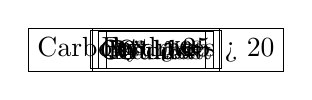
\begin{tikzpicture}[
    node/.style={%
      draw,
      rectangle,
    },
  ]

    \node [node] (A) {Carbohydrates > 20};
    \path (A) ++(-135:\nodeDist) node [node] (B) {Brunost};
    \path (A) ++(-45:\nodeDist) node [node] (C) {Fett > 25};
    \path (C) ++(-135:\nodeDist) node [node] (D) {Gulost};
    \path (C) ++(-45:\nodeDist) node [node] (E) {Gräddost};

    \draw (A) -- (B) node [left,pos=0.25] {yes}(A);
    \draw (A) -- (C) node [right,pos=0.25] {no}(A);
    \draw (C) -- (D) node [left,pos=0.25] {no}(A);
    \draw (C) -- (E) node [right,pos=0.25] {yes}(A);
\end{tikzpicture}
    \caption{A simple example of a decision tree}
    \label{fig:tree}
\end{figure}
In regression analysis, trees are built by a collection of rules based on the available features of the dataset:
\begin{itemize}
    \item Rules based on the values of the variables are selected to obtain the best split to distinguish the observations based on the dependent variable.
    \item Once a rule is selected and a node is split into two parts, the same process is applied to each "child" node (i.e. it is a recursive process).
    \item Splitting stops when the algorithm determines that no further gain can be made or when some preset stop rules are met. (Alternatively, the data is split as much as possible and the tree is pruned later).
\end{itemize}
Each branch of the tree culminates in a terminal node. Each observation falls into exactly one terminal node, and each terminal node defined by a unique set of rules \autocite[][]{breiman1984classification}.
\subsection{Gradient Boosting}
CART are considered weak learners, meaning that their predictive performance is only slightly better than chance. Boosting is a method that can be used to convert weak learners into strong learners. Gradient boosting in particular uses CART as a weak learner. Here, each new tree is an adaptation to a modified version of the original tree. After the first tree is grown, the error residuals, defined as the difference between the target value and the predicted target value, are calculated. A new tree is fitted using the error residuals as the target variable while still using the same input variables. The predicted residuals are added to the previous predictions. This procedure is repeated for the remaining residuals until the loss reaches an acceptable level or no longer improves on an external validation set. \\
Trees are added one at a time and existing trees in the model are not changed. After calculating the loss, a tree must be added that reduces the loss (i.e. follows the gradient). The mathematical version of the algorithm can be seen in Algorithm~\ref{alg:gradient}.
\begin{algorithm}[H]
\caption{The Gradient Boosting Algorithm}
  \label{alg:gradient}
\begin{algorithmic}[1]
\Statex Given a training set $\lbrace\left(x_i,y_i\right)\rbrace_{i=1}^n$, a differentiable loss function $L\left(y, F(x)\right)$ and the number of iterations $M$,
\State Initialization: Compute a model with a constant value:
\begin{equation*}
    F_0\left(x\right)=\underset{\gamma}{\arg\min}\sum_{i=1}^nL\left(y_i,\gamma\right).
\end{equation*}
\For{each iteration $m=1$ to $M$}
    \State Compute \textit{pseudo-residuals}:
    \begin{equation*}
        r_{im}=-\left[\frac{\partial L\left(y_i, F\left(x_i\right)\right)}{\partial F\left(x_i\right)}\right]_{F(x)=F_{m-1}(x)}, \hspace{10pt}\hbox{for } i=1,...,n.
    \end{equation*}
    \State Fit a weak learner $h_m(x)$ to the pseudo-residuals, using $\lbrace\left(x_i,r_{im}\right)\rbrace_{i=1}^n$ as the training set 
    \State Compute the multiplier $\gamma_m$ by solving the following optimization problem:
    \begin{equation*}
        \gamma_m=\underset{\gamma}{\arg\min}\sum_{i=1}^nL\left(y_i,F_{m-1}\left(x_i\right)+\gamma h_m\left(x_i\right)\right).
    \end{equation*}
    \State Update the model:
    \begin{equation*}
        F_m\left(x\right)=F_{m-1}(x)+\gamma_mh_m(x).
    \end{equation*}
    \EndFor
\State Output: $F_M(x)$
\end{algorithmic}
\end{algorithm} $\newline$
Gradient boosting of CART produces robust and interpretable models for both regression and classification that achieve high predictive accuracy \autocite[][]{friedman2001greedy}.
\subsection{Random Forests}
A Random Forest is a classification and regression procedure consisting of several uncorrelated decision trees. All decision trees are grown under a certain type of randomization during the learning process. For a classification, each tree in that forest is allowed to make a decision and the class with the most votes decides the final classification. Random forests can be used for regression. Random forest uses bagging, a meta-algorithm that can be used to improve the stability and accuracy of machine learning algorithms, for instance CART. \\
Using $B$ samples of size $n$, $B$ models $F_i(x), i = 1,..., B$ are computed. For each $x$, $B$ predictions $m_{i}(x), i = 1,...B$ exist then. The predicted value is given by
\begin{equation}
    m^B(x)=\frac{1}{B}\sum_{i=1}^B\left(m_i(x)\right).
\end{equation}
This method, as well as random forest, were both developed by Leo Breiman \autocite[][]{breiman1996bagging}. Random forests differ in only one way from this general scheme: they use a modified tree learning algorithm that selects, at each candidate split in the learning process, a random subset of the features. This process is sometimes called "feature bagging". The reason for doing this is the correlation of the trees in an ordinary bootstrap sample: if one or a few features are strong predictors for the response variable (target output), these features are selected in many of the $B$ trees, causing them to become correlated. A general overview of the random forest is given in Algorithm~\ref{alg:rf}
\begin{algorithm}[H]
\caption{The Random Forest Algorithm}
  \label{alg:rf}
\begin{algorithmic}[1]
\Statex Given a training set $\lbrace\left(x_i,y_i\right)\rbrace_{i=1}^n$, the number of trees $B$ and the number of variables $m$ that should be tried at each split
\State Draw $B$ bootstrap-samples of $\lbrace\left(x_i,y_i\right)\rbrace_{i=1}^n$
\State From the $M$ features of the training data, $m \ll M$ features are randomly selected at each node in the tree to be considered as criteria for the cut (split).
\State Each tree is fully grown and not pruned back
\end{algorithmic}
\end{algorithm} $\newline$
To classify an input, it is evaluated in each tree. The class that is chosen most often is the output of the random forest. In the case of regression, the average prediction is used \autocite[][]{breiman2001random}
\clearpage
\section{Machine Learning Methodology}\label{sec:methods}
After introducing some common machine learning algorithms, this section shows how these algorithms can be optimized to achieve the best possible performance with respect to a given performance measure. Even though machine learning models are often referred to as "black boxes", there are methods to make these models more interpretable. These are presented in this section as well.
\subsection{Tuning of Machine Learning Models}
In the field of machine learning, hyperparameter optimization, also known as hyperparameter tuning, refers to the search for optimal hyperparameters. A hyperparameter is a parameter that is used to control the training algorithm and whose value, unlike other parameters, must be set before the actual training of the model. There exists a variety of methods when it comes to the algorithms used to explore the hyperparameter space, from simple methods like a grid search to Bayesian optimization or more advanced methods like iterated F-racing.
\subsubsection*{Cross-Validation}
Cross-validation is a procedure for evaluating the performance of an algorithm in machine learning. Using new datasets that were not used during the training phase, the goodness of the prediction is examined. This is done by partitioning the known dataset into subsets for training and testing the algorithm and the remaining data.
Each run of cross-validation involves randomly partitioning the original dataset into a training set and a test set. The training data set is used to train a supervised learning algorithm and the test data set is used to evaluate its performance. This process is repeated several times and the mean cross-validation error is used as a performance indicator.
When training a model, it is important not to overfit it with complex algorithms or underfit it with simple algorithms. The choice of training and testing set is critical to reducing this risk. However, it is difficult to split the dataset in a way that maximizes learning and the validity of the test results. This is where cross-validation comes in. To find the best algorithm for the model, cross-validation offers different techniques that split the data differently. \\
A commonly used cross-validation procedure is k-fold cross-validation. In this method, after splitting the original dataset into a training and a test dataset, the training set is split into $k$ subsets called folds. Cross-validation iterates through each fold, using one of the $k$ folds as the validation set at each iteration, while all the remaining folds are used as the training set. This process is repeated until every fold has been used as a validation set. \\
Cross-validation helps to select the best performing model by calculating the error using the test set that is not used for training. The test set is used to calculate model accuracy and show how it generalizes with future data \autocite[][]{fushiki2011estimation}. Figure~\ref{fig:cv} shows an example of 10-fold cross validation.
\begin{figure}[H]
    \centering
    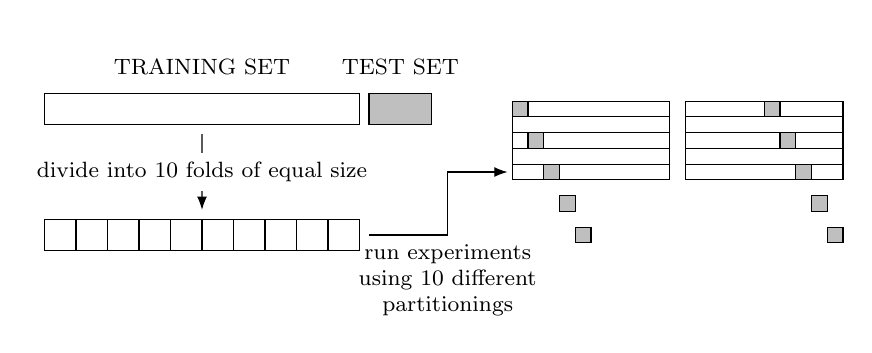
\begin{tikzpicture}[node distance=0mm,minimum height=1cm,outer sep=3mm,scale=0.4,>=Latex,font=\footnotesize,
  indication/.style={minimum height=0cm,outer sep=0mm},
  oneblock/.style={transform shape,minimum width=1cm,draw},
  fullset/.style={transform shape,minimum width=10cm,draw}]
    % left part of picture
    \node[fullset,anchor=west] at (0,0) (A) {};
    \node[above=of A.north,indication] (ATXT) {TRAINING SET};
    \node[oneblock,minimum width=2cm,anchor=west,right=of A,fill=lightgray,outer sep=0mm] (A1) {};
    \path (ATXT) -| (A1) node[midway] {TEST SET};
    \node[fullset,anchor=west] at (0,-4) (B) {};
    \foreach \x in {0,1,...,9}
    {
        \draw (B.west) +(\x,0) node[oneblock,anchor=west,draw] {};
    }
    \draw[->] (A) -- (B) node[midway,fill=white,indication] {divide into 10 folds of equal size};

    % right part of picture
    \begin{scope}[xshift=15cm,scale=0.5,local bounding box=rightside box]
    \foreach \x in {0,1}
    {
        \foreach \y in {0,1,...,4}
        {
            \draw (\x*11,0) +(0,-\y*1) node[fullset,anchor=west] {};
            \draw (\x*11,0) +(\x*5+\y,-\y*2) node[oneblock,draw,anchor=west,fill=lightgray] {};
        }
    }
    \coordinate (R) at (rightside box.west);
    \end{scope}

    % connecting arrow
    \draw[->] (B.east) -- +(2.5,0) node[below,align=center,indication] {run experiments\\using 10 different\\partitionings} |- (R);
  \end{tikzpicture}
    \caption{An example of 10-fold cross validation}
    \label{fig:cv}
\end{figure}
\subsubsection*{Grid and Random Search}
The two most commonly used methods for hyperparameter tuning are grid search and random search. Grid search performs an exhaustive search on a manually defined subset of the learning algorithm's hyperparameter space. A grid search must be guided by a performance metric, typically computed by cross-validation on training data or validation data that is not considered during training. For example, for a knn algorithm, a grid search may try any value for $k$ between 1 and 20 and return the best value for $k$ with respect to a performance measure. One of the major disadvantages of grid search is that it suffers in terms of dimensionality when the number of hyperparameters grows exponentially. With only four parameters, this problem can become impractical as the number of evaluations required for this strategy increases exponentially with each additional parameter due to the curse of dimensionality. \\
In the random search, instead of exhaustively trying all combinations, a random selection of values is made within the given hyperparameter space. Unlike grid search, no discretization of the space is required. Random search can outperform grid search in speed and performance, especially when only a few hyperparameters affect the quality of the learning algorithm. This is because grid search tries only a few values for each parameter (but multiple times), while randomly selected values are much better distributed in the search space \autocite[][]{bergstra2012random}.
\subsubsection*{F-Race and Iterated F-Racing}
F-Race is a racing algorithm that is used to select the best configuration of parameterized algorithms based on statistical approaches. The main idea is to iteratively evaluate a given finite set of candidates on a stream of instances. After each iteration, some candidate configurations that perform significantly worse than others under the Friedman test with post-hoc analysis for pairs are eliminated and only the remaining ones are evaluated for subsequent iterations. The Friedman test is a statistical test for examining three or more paired samples for equality of the location parameter. \\
As this process continues, this method focuses more and more on the most promising candidate configurations. An essential part in F-Race is defining the set of candidate configurations of the first step. One way is iterated F-Race, which creates a probability model for a candidate solution. A set of candidates is evaluated at each iteration to update the probability model and steer the next sample towards the better candidate solutions until a termination criterion is met \autocite[][]{birattari2010f}.
\subsection{Interpretation of Machine Learning Models}
After creating a model, possibly tuning its hyperparameters and finally training it, the logical next step would be to make predictions for unseen data. The accuracy of the predictions can be evaluated using a performance measure such as the mean absolute error. Beyond that, however, it is often quite difficult to interpret the final model or get an idea of why it predicts a particular value given a set of input variables. This is where interpretable machine learning (IML) comes in, as it aims to shed more light into the black box that is most machine learning algorithms.
\subsubsection*{Feature Importance}
The idea behind feature importance is simple. The importance of a feature is measured by calculating the increase in the model's prediction error after permuting the feature. The more the model error is increased by this permutation, the more important a feature is, as this means that the model relies on the feature for prediction. If the model error does not change, a feature is unimportant because the model ignored the feature for prediction. Algorithm~\ref{alg:importance} shows how the algorithm works in practice.
\begin{algorithm}[H]
\caption{The Permutation Feature Importance Algorithm}
  \label{alg:importance}
\begin{algorithmic}[1]
\Statex Given a trained model $F$, a feature matrix $\pmb{X}$, a target vector $\pmb{y}$ and a loss function $L\left(\pmb{y}, F\right)$
\State Estimate the original model error $\varepsilon_{\hbox{\footnotesize orig}}=L\left(\pmb{y}, F(\pmb{X})\right)$
\For{each feature $j=1,...,p$}
    \State Generate permuted feature matrix $\pmb{X}_{\hbox{\footnotesize perm}}$ by permuting feature $j$ in the data $\pmb{X}$, thereby breaking the association between $j$ and the outcome $\pmb{y}$.
    \State Calculate the permutation error $\varepsilon_{\hbox{\footnotesize perm}}=L\left(\pmb{y}, f\left(\pmb{X}_{\hbox{\footnotesize perm}}\right)\right)$ based on the predictions of the permuted data.
    \State Calculate the permutation feature importance $FI_j=\frac{\varepsilon_{\hbox{\footnotesize perm}}}{\varepsilon_{\hbox{\footnotesize orig}}}$.
    \EndFor
\State Sort the features by descending $FI$.
\end{algorithmic}
\end{algorithm} $\newline$
The advantages of feature importance include that it is easy to interpret, it is comparable across different problems, it accounts for all interactions, and it does not require retraining of the model. On the other hand, there is no clear guideline whether it should be used for training or testing data, the true outcome must be known, and the measurement may be biased if the features are correlated \autocite[][]{fisher2018model, molnar2020interpretable}.
\subsubsection*{Partial Dependence Plots}
The partial dependence plot (PDP) shows the marginal effect that one or two features have on the predicted outcome of a machine learning model. A partial dependence plot can reveal whether the relationship between the dependent value and a feature is linear, monotonic or more complex. When applied to a linear regression model, for example, partial dependence plots show a linear relationship every time. \\
For regression, the partial dependence function is given by
\begin{equation}
    \widehat{f}_{\pmb{x}_S}\left(\pmb{x}_S\right)=\mathbb{E}_{\pmb{x}_C}\left[\widehat{f}\left(\pmb{x}_S, \pmb{x}_C\right)\right] = \int\widehat{f}\left(\pmb{x}_S,\pmb{x}_C\right)d\mathbb{P}\left(\pmb{x}_C\right).
\end{equation}
$\pmb{x}_S$ denotes the features for which the partial dependence function is to be plotted and $\pmb{x}_C$ denotes the rest of the features used in the model $\widehat{f}$. In general, the set $S$ contains only one or two features and these are the ones for which the effect on the prediction is to be evaluated. The total feature space $\pmb{x}$ is composed of the feature vectors $\pmb{x}_S$ and $\pmb{x}_C$. By marginalizing the output of $\widehat{f}$ over the distribution of the features in set $C$, the function shows the relationship between the features in $S$ and the predicted outcome. This process produces a function that depends only on the features in $S$ and includes interactions with other features. \\
$\widehat{f}_{\pmb{x}_S}$ is estimated by averaging the training data,
\begin{equation}
    \widehat{f}_{\pmb{x}_S}\left(\pmb{x}\right)=\frac{1}{n}\sum_{i=1}^n\widehat{f}\left(\pmb{x}_S, x_{C, i}\right).
\end{equation}
For given value(s) of $S$, the function returns the average marginal effect on the prediction. $x_{C,i}$ denotes the feature values from the dataset for the features not of interest and $n$ denotes the number of observations in the dataset. For a PDP, it is assumed that the features in $C$ and the features in $S$ are not correlated. Violation of this assumption leads to improbable or impossible data points for the PDP. \\
The advantages of PDPs include clear interpretation and intuitiveness of the method, as the partial dependence function at a given feature value represents the average prediction when all data points are forced to assume that feature value. \\
Disadvantages include the aforementioned assumption of independence and that a maximum of two features can realistically be used, as more than three dimensions are inconceivable to humans \autocite[][]{friedman2001greedy, molnar2020interpretable}.
\subsubsection*{Individual Conditional Expectation}
The PDP for the average impact of a feature is a global method as it does not focus on specific instances but on a total average. The equivalent of a PDP for individual instances of data is called an individual conditional expectation (ICE) plot. An ICE plot visualizes the dependence of the prediction on a feature for each instance separately, leading to one line per instance, compared to the one line in PDPs. Hence, a PDP represents the average of the lines in an ICE plot. The values relating to a line (and one instance) are calculated by keeping the rest of the features the same, producing variants of that instance by replacing the value of the feature with values from a grid, and making predictions using the model for these newly created instances. This results in a set of points for an instance with the feature value from the grid and the respective predictions. \\
Since a PDP only displays the average relationship between a feature and the prediction, heterogeneous relationships arising from interactions can be hidden. If the interactions between the features for which the PDP is calculated and the other features are weak, this is not a problem. However, if these interactions are not weak, an ICE plot provides deeper insight.\\
Formally, for each instance in $\lbrace\left(x_{S,i}, x_{C,i}\right)\rbrace_{i=1}^N$, $\widehat{f}_{S,i}$ is plotted against $x_{S,i}$, where $x_{C,i}$ remains fixed.\\
ICE curves are even more intuitive than a PDP, with each line representing the predictions for an instance when the feature of interest is varied. In addition, they can reveal heterogeneous relationships. \\
Drawbacks include the fact that only one display can be meaningfully plotted, as plotting multiple lines would require drawing multiple overlapping surfaces that would make it difficult to see anything in the plot. It is difficult to see the average and there may be crowding in the plot if too many lines are drawn \autocite[][]{goldstein2015peeking, molnar2020interpretable}
\subsubsection*{Shapley Values}
A prediction can be explained with the assumption that each feature value of the instance is a "player" in a game where the prediction is the payout. A fair distribution of the "payout" among the individual features can be obtained using Shapley values - a methodology from coalitional game theory. The Shapley value, is a method that assigns payouts to players depending on how much they contributed to the total payout. Players cooperate in a coalition and as a result receive a certain profit from this coalition. \\
In machine learning, the "game" is a prediction task for a single observation of the dataset. The difference between the actual prediction of this observation and the average prediction of all instances is the "gain". Feature values of the observation represent the "players" that cooperate to obtain the gain, i.e. to predict a certain value. The Shapley value is thus the average marginal contribution of the value of a feature across all possible coalitions. \\
The Shapley value is given by a value function of the players in $S$. For a single feature value, the Shapley value is its contribution to the payoff, weighted and summed over all possible feature value combinations,
\begin{equation}
    \phi_j\left(\hbox{val}\right)=\sum_{S\subseteq \lbrace x_1,...,x_p\rbrace\setminus \lbrace x_j\rbrace}\frac{\left|S\right|!\left(p-\left|S\right|-1\right)!}{p!}\left(\hbox{val}\left(S\cup\lbrace x_j\rbrace\right)-\hbox{val}(S)\right).
\end{equation}
$S$ denotes a subset of the features used in the model, $\pmb{x}$ is the vector of feature values of the instance to be explained and $p$ stands for the number of features. $\hbox{val}_x(S)$ denotes the prediction for the feature values in $S$ marginalized over features excluded from $S$,
\begin{equation}
    \hbox{val}_{\pmb{x}}(S)=\int\widehat{f}\left(x_1,...,x_p\right)d\mathbb{P}_{\pmb{x}\notin S} - \mathbb{E}_{\pmb{X}}\left[\widehat{f}(\pmb{X})\right].
\end{equation}
In practice, multiple integrations are performed for each feature that is not included in $S$. \\
The definition of a fair allocation can be viewed as an allocation that has four properties: Efficiency, Symmetry, Dummy and Additivity. The only allocation method that satisfies these four properties is the Shapley value. \\
\textbf{Efficiency}: The contributions of the individual features must add up to the difference between the prediction for $\pmb{x}$ and the average prediction,
\begin{equation*}
    \sum_{j=1}^p\phi_j=\widehat{f}(\pmb{x})-\mathbb{E}_{\pmb{X}}\left[\widehat{f}(\pmb{X})\right].
\end{equation*}
\textbf{Symmetry}: Two characteristic values $j$ and $k$ should have the same contribution if their contribution to all possible coalitions is the same. Consequently, if
\begin{equation*}
    \hbox{val}\left(S\cup\lbrace x_j\rbrace\right) = \hbox{val}\left(S\cup\lbrace x_k\rbrace\right)\hspace{10pt}\forall S\subseteq\lbrace x_1,...,x_p\rbrace\setminus\lbrace x_j,x_k\rbrace,
\end{equation*}
then
\begin{equation*}
    \phi_j=\phi_k.
\end{equation*}
\textbf{Dummy}: If a feature $j$ has no influence on the predicted value - regardless of which coalition of feature values it is added to - it should have a Shapley value of 0. Thus if
\begin{equation*}
    \hbox{val}\left(S\cup\lbrace x_j\rbrace\right) = \hbox{val}\left(S\right)\hspace{10pt}\forall S\subseteq\lbrace x_1,...,x_p\rbrace,
\end{equation*}
then
\begin{equation*}
    \phi_j=0.
\end{equation*}
\textbf{Additivity}: For a game that has combined payouts $\hbox{val}+\hbox{val}^+$, the corresponding Shapley values are
\begin{equation*}
    \phi_j+\phi_j^+.
\end{equation*}
Suppose a Random Forest has been trained, i.e. the prediction is an average of many decision trees. The additivity property guarantees that for a feature value the Shapley value can be calculated for each tree separately, averaged and thus the Shapley value for the feature value for the Random Forest is obtained. \\
To calculate the exact Shapley value, all possible coalitions of feature values with and without the $j$-th feature must be evaluated. The more features there are in a dataset, the more problematic this calculation becomes, as the number of possible coalitions increases exponentially. An approximation can be achieved by Monte Carlo sampling,
\begin{equation}
    \widehat{\phi}_j=\frac{1}{M}\sum_{m=1}^M\left(\widehat{f}\left(\pmb{x}_{+j}^m\right)-\widehat{f}\left(\pmb{x}_{-j}^m\right)\right),
\end{equation}
where $\widehat{f}\left(\pmb{x}_{+j}^m\right)$ denotes the prediction for $\pmb{x}$, but where a random number of feature values are replaced by feature values from a randomly drawn data point $\pmb{z}$, except for the respective value of feature $j$. $\pmb{x}_{-j}^m$ is almost identical to $\pmb{x}_{+j}^m$, except that the value $x_j^m$ is also taken from the sample $\pmb{z}$. The calculation of the approximate Shapley value for a single feature value is shown in Algorithm~\ref{alg:shapley}
\begin{algorithm}[H]
\caption{The Estimation of Shapley values for a single feature value}
  \label{alg:shapley}
\begin{algorithmic}[1]
\Statex Given the number of iterations $M$, instance of interest $\pmb{x}$, feature index $j$, data matrix $\pmb{X}$ and machine learning model $f$
\For{each feature $m=1,...,M$}
\State Draw a random instance $z$ from $\pmb{X}$.
\State Choose random permutation $o$ of the feature values.
\State Order $\pmb{x}:\pmb{x}_o=\left(x_1,...,x_j,...,x_p\right)$.
\State Order $\pmb{z}:\pmb{z}_o=\left(z_1,...,z_j,...,z_p\right)$.
\State Construct two new instances
      \begin{algsubstates}
        \State With feature $j:\pmb{x}_{+j}=\left(x_1,...,x_{j-1},x_{j}, z_{j+1},...,z_p\right)$.
        \State Without feature $j: \pmb{x}_{-j}=\left(x_1,...,x_{j-1},z_{j},z_{j+1},...,z_p\right)$.
      \end{algsubstates}
\State Compute the marginal contribution: $\phi_j^m=\widehat{f}\left(\pmb{x}_{+j}\right)-\widehat{f}\left(\pmb{x}_{-j}\right)$
\EndFor
\State Compute the Shapley value through averaging: $\phi_j\left(\pmb{x}\right)=\frac{1}{M}\sum_{m=1}^M\phi_j^m$.
\State Output: The Shapley value for the value of the $j$-th feature.
\end{algorithmic}
\end{algorithm} $\newline$
This process must be repeated for each of the features to obtain each Shapley value. \\
One of the advantages of Shapley values is that the difference between the prediction and the average prediction is evenly distributed among the feature values of the instance, thus fulfilling the property of efficiency. The Shapley value allows for contrastive explanations. Instead of comparing a prediction to the average prediction of the entire dataset, it can be compared to a subset or even a single data point. \\
Among the disadvantages is that the calculation of Shapley values is computationally intensive, as almost always only an approximation is possible. The Shapley value can also be misinterpreted as the difference in predicted value after removing the feature from model training \autocite[][]{shapley1997value, molnar2020interpretable}.

% !TEX root = ../my-thesis.tex
%
\chapter{Dataset Collection}
As is often the case with statisticians, the construction of the dataset used to analyse a research question is an essential task and frequently involves the merging of multiple data sources to create a dataset. This was the case in this thesis and in the following chapter a brief overview of the data sources used, their pre-processing and how they were combined is given.
\label{sec:datacollection}
\clearpage
\section{Covid-19 Data}
\subsection{Covid-19 Data for Norway}
The Covid-19 data for Norway comes from a dataset made available to the public via the a repository on the website \href{https://www.github.com}{Github.com}, created by the user thohan88. The repository contains a daily updated dataset that is the result of combining several data sources, which include the Institute of Public Health and the Norwegian Directorate of Health. According to the author of the repository, the project is "an open-source effort to make data about the Covid-19 situation in Norway available to the public in a timely and coherent manner" \cite{thohan88}. \\
A few sample data points from this dataset are displayed in Table~\ref{datasetNorge}.\\
\begin{table}[H] 
\caption{An excerpt from the Covid-19 data for Norway. Does not contain all variables.\label{datasetNorge}}
\begin{tabular}{l l r r r}
\toprule
\textbf{kommune\_no}	& \textbf{kommune\_name}	& \textbf{population}	& \textbf{2020-03-26}	& \textbf{2020-03-27}\\
\midrule
1103 & Stavanger & 143574 & 87 & 88 \\
1507 & Ålesund & 66258 & 20 & 20 \\
4601 & Bergen & 283929 & 231 & 248 \\
5001 & Trondheim & 205163 & 113 & 136 \\
\bottomrule
\end{tabular}
\end{table}
\subsection{Covid-19 Data for Germany}
In Germany, the Robert Koch Institute publishes daily situation reports in which the number of new cases is published at NUTS 3 level. These reports are available as pdf files via the Institute's website. They can be downloaded and grouped via the R package \texttt{covid19germany}\cite{covid19germany}, as was done for this work.\\
A few sample data points from this dataset are displayed in Table~\ref{datasetGermany}.\\
The variable \textit{CumNumberTestedIll} contains the cumulative number of people that have tested positive for Covid-19.
\begin{table}[H] 
\caption{An excerpt from the Covid-19 data for Germany. Does not contain all variables.\label{datasetGermany}}
\begin{tabular}{l l r r r}
\toprule
\textbf{Landkreis}	& \textbf{Date}	& \textbf{CumNumberTestedIll} & \textbf{population}\\
\midrule
SK München & 2020-01-29 & 1 & 1471508\\
SK München & 2020-02-03 & 2 & 1471508\\
SK München & 2020-02-11 & 3 & 1471508\\
LK Rosenheim & 2020-02-29 & 1 & 260983\\
LK Rosenheim & 2020-03-08 & 2 & 260983 \\
LK Rosenheim & 2020-03-10 & 6 & 260983 \\
\bottomrule
\end{tabular}
\end{table}
\clearpage
\section{Demographic Data}
As demographics tend to differ between different geographic units, the decision was made to include demographic variables in the analysis of the research question to see if the risk for infection may be higher when a certain characteristic is present in the population.
\subsection{Demographic Data for Norway}
The demographic data collected for Norway comes from Statistisk Sentralbyrå and is made available to the public through their online database, StatBank\cite{ssb}. \\
The first characteristic collected was the age of the population in a given municipality. For each age, starting at 0 and ending at 105, the number of people of that age is known. \\
Next, unemployment data were collected for a given municipality. For each municipality, the percentage of all people out of work is known, as well as the percentage of all immigrants out of work. \\
Other data collected include data related to the number of workers in a particular industry, as well as immigration data. Since there is discussion about whether workers from certain industries, in this case construction, contribute to the spread of Covid-19, the decision was made to collect this type of data. For each community, the number of workers across all industries is known, as well as the number of workers in the construction industry. Workers, in this case, are individuals employed in a given municipality who are between the ages of 20 and 66. It is also known how many people work full-time and how many work part-time. \\
Finally, for immigration data, it is known how many immigrants live in a given municipality and how many Norwegians were born to immigrant parents. These figures are known in terms of the percentage of the population in 2020.
\subsection{Demographic Data for Germany}
The demographic data collected for Germany comes from the federal and state statistical offices and is made available to the public through their online database, Regionaldatenbank Deutschland \cite{rdb}. \\
The first characteristic collected was unemployment data at the NUTS 3 level. For each municipality, the number of unemployed people as well as the number of unemployed foreigners was collected. \\
Next, data related to the European elections in 2019 were collected. In each municipality, it is known how many people voted in total, how many people voted for the six largest parties, and how many votes the remaining parties received combined. \\
Data was also collected in relation to people seeking protection, welfare recipients and in relation to asylum seeker benefits. It is known how many people sought protection in Germany, how many received social welfare and how many received asylum seeker benefits. \\
Finally, trade tax, income tax, and payroll tax data were collected for each municipality. 
\clearpage
\section{Shapefiles}
In addition to numeric variables, the dataset also contains a geographic variable containing the geographic boundaries of a given municipality or city/district.
\subsection{Shapefiles for Norway}
The data for the Norwegian shapefiles comes from Geonorge \cite{geonorge} and is downloaded from a Github repository, as the data there was in a cleaner state \cite{shapeGithub}. In addition to the geographic shape, the dataset also includes a variable that contains the ID of each municipality.
\subsection{Shapefiles for Germany}
The data for the German shapefiles comes from Esri Germany \cite{esri}.
\clearpage
\section{OpenStreetMap Data}
OpenStreetMap (OSM) is a free project that collects, structures and stores freely usable geodata in a database for use by anyone (Open Data). This data is available under a free license, the Open Database License. The core of the project is therefore an openly accessible database of all contributed geoinformation \cite{OpenStreetMap}. \\
In R, the OpenStreetMap API can be queried using the R package \texttt{osmdata} \cite{osmdata}. To download all locations of a given type in a given region, a shape or bounding box must be specified along with a key and optionally a value. These key-value pairs are used to specify the type of location, for example, the "amenity" key is used for all facilities used by visitors and residents. If you use the "biergarten" value together with the "amenity" key, the locations of all beer gardens in a given geographic region will be downloaded. \\
OpenStreetMap users have the option to map a location as either \texttt{POINT}, \texttt{POLYGON}, \texttt{MULTIPOLYGON}, \texttt{LINESTRING}, or \texttt{MULTILINESTRING}. Conventionally, the first three are used. Therefore, only sites mapped as one of these were used for this work. If a location was mapped as either \texttt{POLYGON} or \texttt{MULTIPOLYGON}, the centroid of the location was calculated. \\
A complete list of all key-value pairs used for this work can be found in the Appendix. 
\clearpage
\section{Data Wrangling}
The final step before analyzing the research question at hand is to combine all of these data sources into one dataset. This section will show how this was achieved.
\subsection{Data Wrangling for Norway}
The initial step in creating the final dataset was to convert the data from a wide format, as seen in Table~\ref{datasetNorge}, to a long format. This was done using the function \texttt{melt()} from the R package \texttt{reshape2} \cite{reshape2}. The long version of the dataset is shown in Table~\ref{norwayLong}.
\begin{table}[H] 
\caption{An excerpt from the long version of the Norwegian Covid-19 data. Does not contain all variables.\label{norwayLong}}
\begin{tabular}{l l r r r}
\toprule
\textbf{kommune\_no}	& \textbf{kommune\_name}	& \textbf{population} & \textbf{date} & \textbf{value}\\
\midrule
1507 & Ålesund & 66258 & 2020-03-26 & 20\\
5001 & Trondheim  & 205163  & 2020-03-26 & 113\\
1507 & Ålesund & 66258 & 2020-03-27 & 20\\
5001 & Trondheim  & 205163  & 2020-03-27 & 136\\
\bottomrule
\end{tabular}
\end{table}
Next, the demographic data for Norway was loaded and processed. Since the age data contains the number of people of a certain age, the median age was calculated for each region based on how many people of each age group live in each region. \\
The other demographic variables are left unchanged. To combine the demographic data with the Covid-19 data, the municipality IDs were extracted using the \texttt{str\_extract()} function from the \texttt{stringr} \cite{stringr} R package using the regular expression \texttt{[0-9]\{4\}}. Next, all demographic datasets and the Covid-19 dataset were merged using the \texttt{merge()} function. \\
Using the \texttt{st\_intersects()} function from the \texttt{sf} \cite{sf} R package, the number of points of interest downloaded via OpenStreetMap was calculated for each municipality. Since the shapefiles contain the ID for each community, these data were then merged with the data containing the demographic and Covid-19 data. \\
For each variable representing an absolute number, e.g. the number of schools or the number of employees, this number was calculated per 1000 inhabitants of the respective area. \\
If there were missing values in the covariates, these values were imputed using the median of the respective variable. \\
Finally, seven new variables were created:
\begin{itemize}
    \item[1.] expected\_count, which is the expected number of cases in each municipality
    \item[2.] sir, which is the standardised incidence ratio in each municipality
    \item[3.] idarea\_1, which is a unique ID given to each municipality
    \item[4.] higher\_education, which counts the number of universities and colleges in a given area.
    \item[5.] sex, which gives the proportion of females living in a given area.
    \item[6.] pop\_dens, i.e. the number of people per square kilometre in a given area.
    \item[7.] urb\_dens, i.e. the number of residential buildings per square kilometre in a given area.
\end{itemize}
The final dataset contains the variables shown in Table~\ref{datasetNorway}.
\begin{table}[H] 
\caption{The variables contained in the final dataset.\label{datasetNorway}}
\begin{tabular}{l l l}
\toprule
\textbf{Variable Name}	& \textbf{Explanation}	& \textbf{Scale}\\
\midrule
kommune\_no & The municipality ID & None \\
kommune\_name & The municipality name & None \\
population & Population in a municipality & None \\
date & The date of the data used & None \\
value & The number of infected people & None \\
median\_age & The median age & None \\
\multirow{2}{*}{unemp\_tot} & The proportion of &\multirow{2}{*}{[0;1]}\\
& unemployed people \\
\multirow{2}{*}{unemp\_immg} & The proportion of & \multirow{2}{*}{[0;1]}\\
 & unemployed immigrants  \\
\multirow{2}{*}{workers\_ft} & The number of & \multirow{2}{*}{per 1000} \\
& full-time workers \\
\multirow{2}{*}{workers\_pt} & The number of & \multirow{2}{*}{per 1000} \\
& part-time workers \\
\multirow{2}{*}{construction\_ft} & The number of full-time & \multirow{2}{*}{per 1000} \\
& construction workers \\
\multirow{2}{*}{construction\_pt} & The number of part-time & \multirow{2}{*}{per 1000} \\
& construction workers \\
immigrants\_total & The proportion of immigrants  & [0;1] \\
marketplace & The number of marketplaces & per 1000 \\
entertainment & The number of entertainment venues & per 1000 \\
sport & The number of sports amenities & per 1000 \\
clinic & The number of clinics & per 1000 \\
hairdresser & The number of hairdresser & per 1000 \\
shops & The number of shops & per 1000 \\
place\_of\_worship & The number of places of worship & per 1000 \\
retail & The number of retail stores & per 1000 \\
nursing\_home & The number of nursing homes & per 1000 \\
restaurant & The number of restaurants & per 1000 \\
aerodrome & The number of aerodromes & per 1000 \\
office & The number of offices & per 1000 \\
\multirow{2}{*}{platform} & The number of public & \multirow{2}{*}{per 1000} \\
& transport platforms \\
kindergarten & The number of kindergartens & per 1000 \\
schools & The number of schools & per 1000 \\
bakeries & The number of bakeries & per 1000 \\
residential & The number of residential buildings & None \\
\multirow{2}{*}{higher\_education} & The number of colleges & \multirow{2}{*}{per 1000} \\
& and universities \\
expected\_count & The expected number of infections & None \\
sir & The standardised incidence ratio & None \\
idarea\_1 & A unique ID & None \\
area & The area in km$^2$ & None \\
pop\_dens & The population density & People per km$^2$ \\
\multirow{2}{*}{urb\_dens} & \multirow{2}{*}{The urban density}  & Residential buildings\\
& & per km$^2$\\
sex & The proportion of females & [0;1] \\
\bottomrule
\end{tabular}
\end{table}
\subsection{Data Wrangling for Germany}
The data processing procedure for Germany is identical to that for Norway. First, all demographic variables were loaded and left unchanged before being merged with the Covid-19 data prior to calculating the spatial intersections between the points of interest and the NUTS-3 areas. After merging all the data, the numbers per 1000 inhabitants were calculated for the variables containing absolute numbers. For the variables containing the number of people who voted for a particular political party, the relative percentage of votes the party received was calculated. Again, missing values were imputed using the median.
Finally, the same seven new variables were created. 
The final dataset contains the variables shown in Table~\ref{finalGermany}.
\begin{table}[H] 
\caption{The variables contained in the final dataset.\label{finalGermany}}
\begin{tabular}{l l l}
\toprule
\textbf{Variable Name}	& \textbf{Explanation}	& \textbf{Scale}\\
\midrule
municipality\_id & The municipality ID & None\\
municipality & The municipality name & None \\
population & Population in a municipality & None \\
date & The date of the data used & None\\
value & The number of infected people & None \\
trade\_tax & The trade tax in Euros & per 1000 \\
income\_tax & The income tax in Euros & per 1000 \\
income\_total & The income and payroll tax in Euros & per 1000 \\
\multirow{2}{*}{asyl\_benefits} & The number of people & \multirow{2}{*}{per 1000} \\
& receiving asylum seeker benefits \\
welfare\_recipients & The number of welfare recipients & per 1000 \\
unemployed\_total & The number of unemployed people & per 1000 \\
unemployed\_foreigners & The number of unemployed foreigners & per 1000 \\
protection\_seekers & The number of protection seekers & per 1000 \\
Union & Percentage of vote for Union & [0;1]\\
SPD & Percentage of vote for SPD & [0;1]\\
Gruene & Percentage of vote for Gruene & [0;1]\\
FDP & Percentage of vote for FDP & [0;1]\\
die\_linke & Percentage of vote for die Linke & [0;1]\\
afd & Percentage of vote voted for AfD & [0;1] \\
marketplace & The number of marketplaces & per 1000 \\
entertainment & The number of entertainment venues & per 1000 \\
sport & The number of sports amenities & per 1000 \\
clinic & The number of clinics & per 1000 \\
hairdresser & The number of hairdresser & per 1000 \\
shops & The number of shops & per 1000 \\
place\_of\_worship & The number of places of worship & per 1000 \\
retail & The number of retail stores & per 1000 \\
nursing\_home & The number of nursing homes & per 1000 \\
restaurant & The number of restaurants & per 1000 \\
aerodrome & The number of aerodromes & per 1000 \\
office & The number of offices & per 1000 \\
\multirow{2}{*}{platform} & The number of public & \multirow{2}{*}{per 1000} \\
& transport platforms \\
kindergarten & The number of kindergartens & per 1000 \\
schools & The number of schools & per 1000 \\
bakeries & The number of bakeries & per 1000 \\
residential & The number of residential buildings & None \\
\multirow{2}{*}{higher\_education} & The number of colleges & \multirow{2}{*}{per 1000} \\
& and universities \\
expected\_count & The expected number of infections & None \\
sir & The standardised incidence ratio & None \\
idarea\_1 & A unique ID & None \\
area & The area in km$^2$ & None \\
pop\_dens & The population density & People per km$^2$ \\
\multirow{2}{*}{urb\_dens} & \multirow{2}{*}{The urban density}  & Residential buildings\\
& & per km$^2$\\
sex & The proportion of females & [0;1] \\
\bottomrule
\end{tabular}
\end{table}
% !TEX root = ../my-thesis.tex
%
\chapter{Data Analysis}
\label{sec:analysis}
In this chapter the models calculated for each country are reviewed. First, a look at the standardised incidence rate for each country is taken, before spatial models, spatio-temporal models and finally predictive models are discussed.
\section{Standardised Incidence Ratio}
This section takes a brief look at the standardised incidence ratio for the countries of interest.
\subsection{Standardised Incidence Ratio for Germany}
When looking at the standardised incidence ratio for Germany, it is noticeable that the actual number of infections in the eastern parts of Germany, especially in Saxony, is considerably higher than the expected number of infections. Furthermore, parts of Bavaria have an increased standardised incidence ratio compared to the rest of Germany, excluding Saxony. This could be due to the fact that the regions share a border with the Czech Republic, a country that is substantially more affected by Covid-19 than Germany. The northern parts of Germany show the lowest SIR which is possibly due to the fact that this region is sparsely populated. For more information, see Figure~\ref{sirgermany}.
% \begin{figure}[H]
%   \centering
%   \includesvg[width = 1.2\textwidth]{sir_germany.svg}
%   \caption{The standardised incidence ratio for Germany based on the data of the 18th of March 2021}
%   \label{sirgermany}
% \end{figure}
\begin{figure}[H]
  \centering
  \includegraphics[width = 1.2\textwidth]{sir_germany.png}
  \caption{The standardised incidence ratio for Germany based on the data of the 18th of March 2021}
  \label{sirgermany}
\end{figure}
\subsection{Standardised Incidence Ratio for Norway}
Looking at the standardised incidence rate for Norway, a standardised incidence rate of less than 1 can be seen for most municipalities north of Trondheim. In the southern parts of Norway there are several municipalities with a rate above 1, for example the standardised incidence rate around the capital Oslo is around 2. However, the two small municipalities, Hyllestad and Ulvik, have the highest standardised incidence rate in Norway. In Hyllestad, 95 of 1328 people have been infected with Covid-19 so far, while in Ulvik, 134 of 1080 people have been infected so far. \\
The SIR in Hyllestad is around 4.5, following an outbreak in a shipyard in autumn 2020 \cite{newspaper1}, while Ulvik has a ratio of around 8, following an outbreak of the UK variant of Covid-19. According to the head of the municipality, Hans Petter Thorbjørnsen, the infections are thought to have spread through children \cite{newspaper2}. See Figure~\ref{sirnorway} for more information.
% \begin{figure}[H]
%   \centering
%   \includesvg[width = 1.2\textwidth]{sir_norway.svg}
%   \caption{The standardised incidence ratio for Norway based on the data of the 20th of March 2021}
%   \label{sirnorway}
% \end{figure}
\begin{figure}[H]
  \centering
  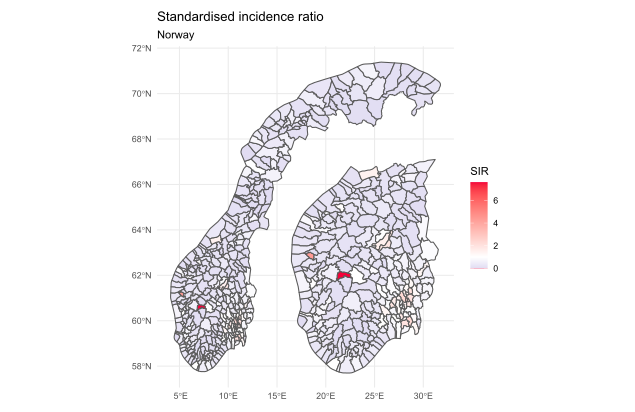
\includegraphics[width = 1.2\textwidth]{sir_norway.png}
  \caption{The standardised incidence ratio for Norway based on the data of the 20th of March 2021}
  \label{sirnorway}
\end{figure}
Because the high numbers from two small municipalities complicate the interpretation of Figure~\ref{sirnorway}, Figure~\ref{sirnorwaylog} shows the SIR on a log10 scale. It is now clearer that the standardized incidence ratio is below 1 in most parts of Norway, but that there is a higher risk in the region around Oslo.
% \begin{figure}[H]
%   \centering
%   \includesvg[width = 1.2\textwidth]{sir_norway_log.svg}
%   \caption{The log10 standardised incidence ratio for Norway based on the data of the 20th of March 2021}
%   \label{sirnorway}
% \end{figure}
\begin{figure}[H]
  \centering
  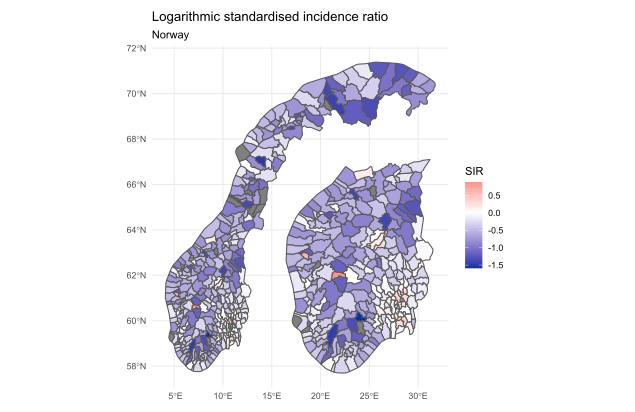
\includegraphics[width = 1.2\textwidth]{sir_norway_log.png}
  \caption{The log10 standardised incidence ratio for Norway based on the data of the 20th of March 2021}
  \label{sirnorwaylog}
\end{figure}
\clearpage
\section{Spatial Models}
After looking at the standardised incidence rates for the countries of interest, the next step is to take a closer look at the current figures for the respective countries. Spatial models are used to try to extract the factors that cause some populations to be at higher risk than other populations. Three different types of models are used for each country:
\begin{itemize}
    \item[1.] The Besarg-Yollie-Mollie Model
    \item[2.] Besags Proper Spatial Model
    \item[3.] The Leroux-Model
\end{itemize}
All of these models were computed using the INLA \cite{rinla} R package. \\
To specify each type of model, the code shown in Listing~\ref{codeModels} can be used. \\
Three measures are used to compare the models, the DIC, the WAIC and the CPO. \\
For all countries, the models were computed with
\begin{itemize}
    \item[1.] only the demographic variables as covariates
    \item[2.] only the infrastructural variables as covariates
    \item[3.] both, demographic and infrastructural variables, as covariates
    \begin{itemize}
        \item[3.1] Without variable selection
        \item[3.2] With variable selection
    \end{itemize}
\end{itemize}
For each model type, different values for the penalised prior were tried. As this resulted in a large number of models, only the model with the best performance for each model class is examined in more detail. \\
The models were compared using the mean absolute error. For this, 20\% of the observations were removed from the training and used for testing instead. The predicted number of infections for these municipalities was then compared to the actual numbers.
\\
Finally, due to the amount of covariates, forwards and backwards stepwise variable selection was performed with the intention of obtaining a model that fits the data well and at the same time is relatively easy to interpret. This can be done with the R package \texttt{INLAutils} \cite{inlautils}, as shown in Listing~\ref{codeSelection}. Backwards as well forwards variable selection was performed.\\
A list of all calculated models along with their performance measures is provided in the appendix.
\subsection{Model Selection}
Before the models are computed, however, the distribution that fits the number of cases must first be found. For this, the function \texttt{descdist()} from the \texttt{fitdistrplus} R package is used. The Cullen and Frey graph can be used to give an initial idea of which distributions fit the data, in this case the number of infections, reasonably well depending on the kurtosis and the square of the skewness. \\
The plots for Germany and Norway can be seen in Figure~\ref{cf_germany} and Figure~\ref{cf_norge}.
% \begin{figure}[H]
%     \centering
%     \includesvg[width = 0.8\textwidth]{cf_germany.svg}
%     \caption{The Cullen and Frey graph for Germany}
%     \label{cf_germany}
% \end{figure}
\begin{figure}[H]
    \centering
    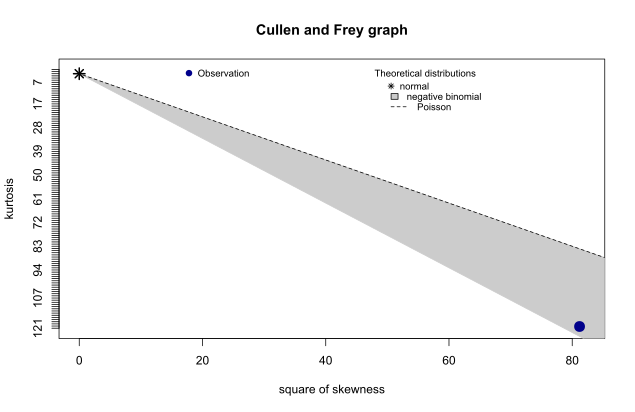
\includegraphics[width = 0.8\textwidth]{cf_germany.png}
    \caption{The Cullen and Frey graph for Germany}
    \label{cf_germany}
\end{figure}
% \begin{figure}[H]
%     \centering
%     \includesvg[width = 0.8\textwidth]{cf_norge.svg}
%     \caption{The Cullen and Frey graph for Norway}
%     \label{cf_norge}
% \end{figure}
\begin{figure}[H]
    \centering
    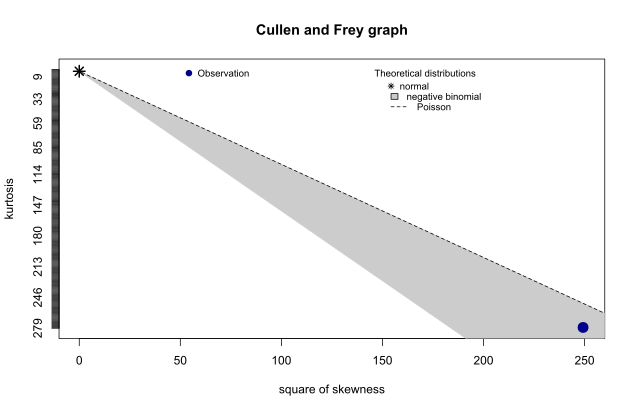
\includegraphics[width = 0.8\textwidth]{cf_norge.png}
    \caption{The Cullen and Frey graph for Norway}
    \label{cf_norge}
\end{figure}
Next, a negative binomial distribution, a normal distribution, and a Poisson distribution are fitted to the data using the maximum likelihood method. The negative binomial fits for both countries can be seen in Figure~\ref{fitNegbinomGermany} and Figure~\ref{fitNegbinomNorway}. The fits for the normal and Poisson distribution for both countries, are shown in the Appendix in Figure~\ref{fitNormalGermany}, Figure~\ref{fitPoissonGermany}, Figure~\ref{fitNormalNorway} and Figure~\ref{fitPoissonNorway}.
% \begin{figure}[H]
%     \centering
%     \includesvg[width = 0.8\textwidth]{fit_nbinom_germany.svg}
%     \caption{A negative binomial fit to the number of cases in German municipalities}
%     \label{fitNegbinomGermany}
% \end{figure}
\begin{figure}[H]
    \centering
    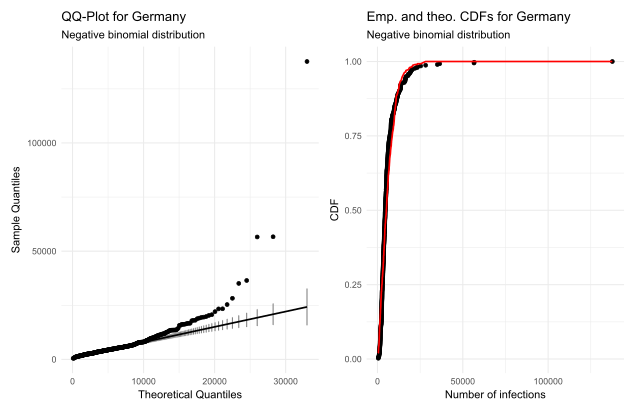
\includegraphics[width = 0.8\textwidth]{fit_nbinom_germany.png}
    \caption{A negative binomial fit to the number of cases in German municipalities}
    \label{fitNegbinomGermany}
\end{figure}
% \begin{figure}[H]
%     \centering
%     \includesvg[width = 0.8\textwidth]{fit_nbinom_norway.svg}
%     \caption{A negative binomial fit to the number of cases in Norwegian municipalities}
%     \label{fitNegbinomNorway}
% \end{figure}
\begin{figure}[H]
    \centering
    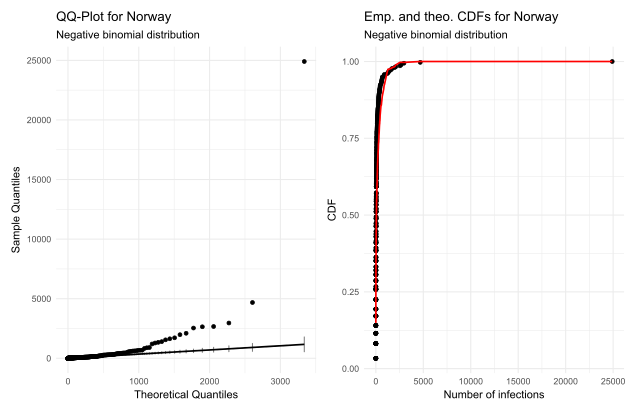
\includegraphics[width = 0.8\textwidth]{fit_nbinom_norway.png}
    \caption{A negative binomial fit to the number of cases in Norwegian municipalities}
    \label{fitNegbinomNorway}
\end{figure}
Lastly, the AIC was calculated for fitting a normal distribution to the data, a Poisson distribution to the data and a negative binomial distribution to the data. The values can be seen in Table~\ref{aic}. Afterwards, the negative binomial distribution was chosen as the distribution of the target variable in both cases. \\
\begin{table}[H] 
\caption{The AIC for different distributions for Germany and Norway \label{aic}}
\begin{tabular}{l l r}
\toprule
\textbf{Country}	& \textbf{Distribution}	& \textbf{AIC} \\
\midrule
Germany & Normal & 8360 \\
Germany & Poisson & 2148100 \\
Germany & Negative Binomial & 7731 \\
Norway & Normal & 6166 \\
Norway & Poisson & 366181 \\
Norway & Negative Binomial & 4086 \\
\bottomrule
\end{tabular}
\end{table} 
The poor fit for the Poisson distribution can be explained by looking at the range of the number of confirmed cases in a given municipality. For Germany, this number ranges from 508 to 137634 (as of March 18, 2021), while for Norway, the number ranges from 0 to 24905 (as of March 20, 2021). This results in a mean and standard deviation for Germany of 6617 and 9014, respectively. For Norway, the values for these metrics are 236 and 1389.
\subsection{Spatial Models for Germany}
First, a look is taken at the spatial models calculated for Germany. These models are based on data from 18 March 2021, when 2.669.233 people in Germany were confirmed infected with Covid-19. The five municipalities with the most infections are shown in Table~\ref{top5germany}.
\begin{table}[H] 
\caption{The municipalities with the most infections as of March 18th 2021. \label{top5germany}}
\begin{tabular}{l r r}
\toprule
\textbf{Municipality}	& \textbf{Population}	& \textbf{Number of infections} \\
\midrule
SK Berlin & 3644826 & 137634 \\     
SK Hamburg & 1841179 & 56656 \\
SK Munich & 1471508 & 56559 \\
SK Cologne & 1085664 & 36455 \\
Region Hannover & 1157624 & 35097 \\
\bottomrule
\end{tabular}
\end{table}
\subsubsection{Demographic Models}\label{sssec:demoGermany}
The model with the best performance based on the demographic variables was a Leroux model calculated formula in Listing~\ref{codeDemoGermany}. The variables used for this model were the percentages of the vote for the six biggest German political parties. \\
The performance measures of this model and the best-performing BYM2 and Besag proper models are shown in Table~\ref{demoGermany}. 
\begin{table}[H] 
\caption{The performance measures for the best performing demographic model of each type. \label{demoGermany}}
\begin{tabular}{l r r r r}
\toprule
\textbf{Model}	& \textbf{DIC}	& \textbf{WAIC} & \textbf{CPO} & \textbf{MAE}\\
\midrule
Besag  & 4598 & 4598 & -2715 & 219618 \\
BYM2 & 4535 & 4502 & -2704 & 219109\\
Leroux & 4685  & 4716 & -2976 & 216908\\
\bottomrule
\end{tabular}
\end{table}
The summary of the fixed effects is shown in Table~\ref{fixedDemoGermany}. To compute the posterior mean of the coefficients, the code shown in Listing~\ref{codePosteriorMean} can be used. \\
To obtain a credibility interval of the fixed effects on the transformed scale, the code in Listing~\ref{codeCredibility} can be used. \\
\begin{table}[H] 
\caption{The fixed effects for the Leroux model. Values are rounded. \label{fixedDemoGermany}}
\begin{tabular}{l r r r r}
\toprule
\textbf{Variable}	& \textbf{Mean}	& \textbf{exp(mean$_{\hbox{p}}$)} & \textbf{exp(q0025$_{\hbox{p}}$)} & \textbf{exp(q0975$_{\hbox{p}}$)} \\
\midrule
(Intercept) & -0.07733 & 0.9257 & 0.8953 & 0.9568 \\
Union & -0.1307 & 0.8804 & 0.7485 & 1.029 \\
SPD & -0.1597 & 0.8531 & 0.7842 & 0.9264 \\
Gruene & -0.1055 & 0.9022 & 0.7812 & 1.036 \\
FDP & 0.001426 & 1.002 & 0.9630 & 1.041 \\
die\_linke & -0.1930 & 0.8254 & 0.7505 & 0.9057 \\
afd & 0.1377 & 1.150 & 1.005 & 1.311 \\
\bottomrule
\end{tabular}
\end{table}
The posterior mean of the exponentiated intercept implies a -7.43\% risk rate across Germany with a credibility interval ranging from -10.47\% to 4.32\%.  \\
This summary shows that especially people who come from regions where the AfD gets a higher share of the vote have a higher risk of contracting Covid-19. In Figure~\ref{sirgermany}, regions in eastern Germany often had a higher SIR. These are also the regions where the AfD tends to perform better in elections. The connection between the two can be attributed to the fact that the AfD is a right-wing party that openly criticises the measures taken to prevent the spread of the coronavirus. As a result, a large proportion of people who vote for the AfD do not take the measures seriously either and refuse to keep a safe distance or wear a mask in public spaces. \\
A one standard deviation increase for the AfD leads to a risk increase of about 15\%. The only other party with a posterior mean greater than 1 is the liberal FDP, which is known for its capitalist views. An increase of one standard deviation increases the risk by 0.16\%. \\
As for the rest of the parties, they are either the leading party in Germany (Union) or left-wing oriented (SPD, the Greens and the Left). People who vote for left-wing parties may respect the Corona rules more and show more consideration for other people.
As this was the overall best-performing spatial model for Germany, a look is taken at the posterior means $\pmb{\zeta} = \exp{\left(\xi\right)}$ of the area-specific risks. Since the uncertainty associated with them can also be mapped, the posterior probability $\mathbb{P}\left(\zeta_i > 1|y\right)$ is visualised as well. In Figure~\ref{posteriorGermany} it can be seen that the relative risk is higher in the south-eastern parts of Bavaria as well as in parts of Saxony, North Rhine-Westphalia and Brandenburg. The posterior probability for these regions is mostly between 0.75 and 1. Both Saxony and Brandenburg are political strongholds for the AfD, while North Rhine-Westphalia is home to the Ruhr region, Germany's most populous metropolitan area. The higher numbers in Bavaria can be explained by the large common borders with Austria and the Czech Republic, two countries that were more affected by the pandemic. Many people cross these borders because of tourism and many guest workers come from the Czech Republic to work on agricultural land in Bavaria, which resulted in several Covid-19 outbreak events.
\begin{figure}[H]
    \centering
    \includegraphics[width = \textwidth]{posterior_germany.png}
    \caption{Posterior mean of the area-specific risk and the posterior probability.}
    \label{posteriorGermany}
\end{figure}
% \begin{figure}[H]
%     \centering
%     \includesvg[width = textwidth]{posterior_germany.svg}
%     \caption{A negative binomial fit to the number of cases in Norwegian municipalities}
%     \label{nb_norge}
% \end{figure}
\subsubsection{Infrastructure Models}
When it comes to the models based on the infrastructural variables, a BYM2 model performed the best. It was computed using formula in Listing~\ref{codeInfraGermany}. \\
The performance measures of this model and the best-performing Besag proper and Leroux model are shown in Table~\ref{infraGermany}
\begin{table}[H] 
\caption{The performance measures for the best performing demographic model of each type. \label{infraGermany}}
\begin{tabular}{l r r r r}
\toprule
\textbf{Model}	& \textbf{DIC}	& \textbf{WAIC} & \textbf{CPO} & \textbf{MAE}\\
\midrule
Besag & 4604 & 4598 & -2742 & 232444\\
BYM2 & 4561 & 4539 & -2714 & 230728\\
Leroux & 4727 & 4754 & -3318 & 238526\\
\bottomrule
\end{tabular}
\end{table}
The values of the covariates are shown in Table~\ref{fixedInfraGermany}.
\begin{table}[H] 
\caption{The fixed effects for the BYM2 model. Values are rounded. \label{fixedInfraGermany}}
\begin{tabular}{l r r r r}
\toprule
\textbf{Variable}	& \textbf{Mean}	& \textbf{exp(mean$_{\hbox{p}}$)} & \textbf{exp(q0025$_{\hbox{p}}$)} & \textbf{exp(q0975$_{\hbox{p}}$)} \\
\midrule
(Intercept) & -0.07275 & 0.9299 & 0.9168 & 0.9430 \\
shops & 0.1590 & 1.179 & 0.9487 & 1.448 \\
hairdresser & 0.1554 & 1.172 & 1.003 & 1.360 \\
marketplace & 0.03241 & 1.034 & 0.9663 & 1.104 \\
schools & 0.03174 & 1.034 & 0.9325 & 1.143 \\
nursing\_home & 0.006124 & 1.006 & 0.9775 & 1.036 \\
bakeries & 0.005910 & 1.009 & 0.8563 & 1.181 \\
place\_of\_worship & 0.001925 & 1.002 & 0.9591 & 1.047 \\
entertainment & -0.01105 & 0.9907 & 0.8812 & 1.110 \\
retail & -0.01147 & 0.9892 & 0.9235 & 1.058 \\
aerodrome & -0.01204 & 0.9884 & 0.9368 & 1.042 \\
sport & -0.01208 & 0.9888 & 0.9151 & 1.067 \\
higher\_education & -0.02014 & 0.9803 & 0.9420 & 1.020 \\
office & -0.03995 & 0.9615 & 0.8942 & 1.032 \\
platform & -0.04970 & 0.9519 & 0.8971 & 1.009 \\
clinic & -0.05596 & 0.9460 & 0.8929 & 1.001 \\
kindergarten & -0.09283 & 0.9143 & 0.7797 & 1.065 \\
restaurant & -0.1094 & 0.8984 & 0.7877 & 1.020 \\
\bottomrule
\end{tabular}
\end{table}
Some findings from these results are that shops, defined as supermarkets, convenience stores and drugstores, hairdressers, marketplaces, schools, nursing homes, bakeries and places of worship all increase the risk of infection. The two highest are shops and hairdressers, where a 1 standard deviation increase leads to a 17.9\% increase in risk in the case of shops and a 17.2\% increase in risk for hairdressers. It should not be surprising that shops in particular increase the risk of infection, as people tend to congregate there and people living in areas where a supermarket is nearby may prefer to go shopping more often to buy fresh produce rather than just once a week when a supermarket is further away. \\
In Germany, there was a big discussion about whether hairdressers should be allowed to stay open during lockdowns, as they were forced to close and could only work when there was no lockdown. Seeing how much hairdressers increase the risk of infection, it might have been a wise decision not to allow them to continue working during a closure. \\
Finally, the number of schools in a given community also increases the risk of infection. An increase of 1 standard deviation increases the risk by about 3.4\%.
\\
There are also effects that have a posterior mean of less than 1, suggesting that they reduce the risk of infection. However, this is not necessarily the case, as it is probably safer for a person to stay at home than to go to a restaurant, for example. It is interesting to note, however, that the lowest posterior mean was observed for restaurants. This could be due to the fact that during most of the time restaurants were either only allowed to serve take-away food or had very strict hygiene policies. The low value could indicate that these measures worked as intended.
\subsubsection{Combined Models}
Finally, models are considered that include both the infrastructural and demographic covariates. Due to the amount of variables, all models run are based on variable selection. \\
The best performing model was again a BYM2 model, run with the formula shown in Listing~\ref{codeBothGermany}. \\
The performance measures of the computed models are shown in Table~\ref{allGermany}.
\begin{table}[H] 
\caption{The performance measures for the best performing demographic model of each type. \label{allGermany}}
\begin{tabular}{l r r r r}
\toprule
\textbf{Model}	& \textbf{DIC}	& \textbf{WAIC} & \textbf{CPO} & \textbf{MAE}\\
\midrule
Besag&  4628 & 4605 & -2673 & 249901\\
BYM2 & 4580 & 4571 & -2683 & 247323\\
Leroux & 4764 & 4791 & -2833 & 248031 \\
\bottomrule
\end{tabular}
\end{table}
The fixed effects are shown in Table~\ref{fixedAllGermany}.

\begin{table}[H] 
\caption{The fixed effects for the BYM2 model. Values are rounded. \label{fixedAllGermany}}
\begin{tabular}{l r r r r}
\toprule
\textbf{Variable}	& \textbf{Mean}	& \textbf{exp(mean$_{\hbox{p}}$)} & \textbf{exp(q0025$_{\hbox{p}}$)} & \textbf{exp(q0975$_{\hbox{p}}$)} \\
\midrule
(Intercept) & -0.07327 & 0.9294 & 0.9149 & 0.9438 \\
afd & 0.2488 & 1.283 & 1.213 & 1.356 \\
pop\_dens & 0.1196 & 1.127 & 1.078 & 1.178 \\
schools & 0.04867 & 1.051 & 0.9586 & 1.150 \\
welfare\_recipients & 0.04565 & 1.048 & 0.9579 & 1.143 \\
sport & 0.02466 & 1.026 & 0.9586 & 1.096 \\
place\_of\_worship & -0.0002002 & 1.000 & 0.9633 & 1.038 \\
nursing\_home & -0.0006482 & 0.9994 & 0.9752 & 1.024 \\
kindergarten & -0.002457 &  0.9993 & 0.8898 & 1.119 \\
log(trade\_tax) & -0.006766 & 0.9933 & 0.9705 & 1.016 \\
FDP & -0.01635 & 0.9840 & 0.9453 & 1.024 \\
office & -0.01770 & 0.9830 & 0.9178 & 1.051 \\
bakeries & -0.02426 & 0.9780 & 0.8627 & 1.1104 \\
platform & -0.03003 & 0.9708 & 0.9186 & 1.025 \\
entertainment & -0.04251 & 0.9594 & 0.8763 & 1.048 \\
SPD & -0.05188 & 0.9497 & 0.9088 & 0.9919 \\
die\_linke & -0.1284 &  0.8799 & 0.8288 & 0.9333\\
\bottomrule
\end{tabular}
\end{table}
According to this model, the three biggest driving factors are the percentage of votes the AfD receives, the population density and the number of schools in a municipality. The influence of the AfD and the number of schools has already been discussed in section~\ref{sssec:demoGermany}. Regarding population density, it can be said that if it increases by 1 standard deviation, the risk of infection increases by 12.7\%. The more people are concentrated per square kilometre, the easier it is for a virus to spread because the distances between people become smaller. Other factors that positively influence the risk of infection are the number of social welfare recipients, the number of sports facilities and the number of places of worship, although the risk increase for the latter is only just above 0. Sports facilities are again a place where many people come together, and here, depending on the type of sport, there can also be more contact, which in turn favours the spread of a virus. The last effect worth mentioning is the logarithmic business tax. If a region receives more revenue through business tax, the risk of infection in that region decreases. Therefore, people in communities where there is less money are at higher risk. 
\subsection{Spatial Models for Norway}
Next, the same types of models are evaluated for Norway. These models are based on data from 12 March 2021, when 76577 people in Norway were confirmed infected with Covid-19. The five municipalities with the most infections are shown in Table~\ref{top5norway}.
\begin{table}[H] 
\caption{The municipalities with the most infections as of March 12th 2021. \label{top5norway}}
\begin{tabular}{l r r}
\toprule
\textbf{Municipality}	& \textbf{Population}	& \textbf{Number of infections} \\
\midrule
Oslo & 693494 & 22248 \\
Bergen & 283929 & 4618 \\
Drammen & 101386 & 2549 \\
Lillestrøm & 85983 & 2390 \\
Fredrikstad & 82385 & 2373 \\
\bottomrule
\end{tabular}
\end{table}
\subsubsection{Demographic Models}
As with Germany, the best demographic model was again a Leroux model. Only this time, the covariates of the model were selected using forwards variable selection. The following formula was used for the model:
\begin{lstlisting}[caption={The formula for the best Leroux model based on the demographic variables}, label={codeDemoNorway}, language = R]
formula_22_leroux <- value ~
  pop_dens + immigrants_pure + median_age +
  sex +
  f(
    idarea_1, model = "generic1",
    Cmatrix = C, hyper = prior_2
  )
\end{lstlisting}
The performance measures for all three types of models are shown in Table~\ref{demoNorway}.
\begin{table}[H] 
\caption{The performance measures for the best performing demographic model of each type. \label{demoNorway}}
\begin{tabular}{l l l l}
\toprule
\textbf{Model}	& \textbf{DIC}	& \textbf{WAIC} & \textbf{CPO} \\
\midrule
Besags Proper  & 2804 (45) & 2820 (45) & -10433 (23) \\
BYM2 & 2716 (3) & 2670 (14) & -9786 (25)\\
Leroux & 2703 (1) & 2648 (1) & -11077 (14) \\
\bottomrule
\end{tabular}
\end{table}
The Leroux model had the best performance in terms of both DIC and WAIC and also performed well in terms of CPO. Just like for Germany, a total of 66 models were calculated. Of the 14 best models in terms of CPO, 13 were Leroux models. \\
The effects of the covariates are shown in Table~\ref{fixedDemoNorway}.
\begin{table}[H] 
\caption{The fixed effects for model 22. Values are rounded. \label{fixedDemoNorway}}
\begin{tabular}{l r r r r}
\toprule
\textbf{Variable}	& \textbf{Mean}	& \textbf{exp(mean$_{\hbox{p}}$)} & \textbf{exp(q0025$_{\hbox{p}}$)} & \textbf{exp(q0975$_{\hbox{p}}$)} \\
\midrule
(Intercept) & 1.087 & 222.4 & -8.203e+09 & -9.140e+04\\
pop\_dens & 0.001775 & 1.002 & 1.001 & 1.003\\
immigrants\_pure & -0.03358 & 0.9671 & 0.9392 & 0.9948\\
median\_age & -0.03628  & 0.9645 & 0.9396 & 0.9897\\
sex & -0.0426 & 2.902e+06 & -6.904e+26 & -1.164e+22 \\
\bottomrule
\end{tabular}
\end{table}
There is little meaningful interpretation for the posterior mean of the intercept in this model due to its high value. Of note is that if the population density increases by 100 persons per square kilometre, the risk of infection increases by about 19.4\%. Furthermore, if the proportion of women in an area increases by 0.05, the risk of infection increases by around 7.7\%. Finally, if the average age in a community increases by 1 year, the risk of infection decreases by roughly 3.5\%. Because younger people tend to be more mobile, they come into contact with more people than older generations, so it makes sense that people living in younger areas have a higher risk of becoming infected with Covid-19.
\subsubsection{Infrastructure Models}
Looking at the 24 models computed for Norway that are based on the infrastructural variables, once again a Leroux model based on forwards variable selection had the best performance. The formula is shown in Listing~\ref{codeInfraNorway}.
\begin{lstlisting}[caption={The formula for the best Leroux model based on the infrastructural variables}, label={codeInfraNorway}, language = R]
formula_30_leroux <- value ~
  pop_dens + shops + retail + place_of_worship +
  schools + nursing_home + kindergarten +
  f(
    idarea_1, model = "generic1",
    Cmatrix = C, hyper = prior_2
  )
\end{lstlisting}
The performance measure for the models are shown in Table~\ref{infraNorway}.
\begin{table}[H] 
\caption{The performance measures for the best performing demographic model of each type. \label{infraNorway}}
\begin{tabular}{l l l l}
\toprule
\textbf{Model}	& \textbf{DIC}	& \textbf{WAIC} & \textbf{CPO} \\
\midrule
Besags Proper  & 2816 (17) & 2813 (17) & -10347 (8) \\
BYM2 & 2728 (2) & 2671 (2) & -9145 (14)\\
Leroux & 2718 (1) & 2665 (1) & -9553 (11) \\
\bottomrule
\end{tabular}
\end{table}
The effect of the covariates are shown in Table~\ref{fixedInfraNorway}.
\begin{table}[H] 
\caption{The fixed effects for model 30. Values are rounded. \label{fixedInfraNorway}}
\begin{tabular}{l r r r r}
\toprule
\textbf{Variable}	& \textbf{Mean}	& \textbf{exp(mean$_{\hbox{p}}$)} & \textbf{exp(q0025$_{\hbox{p}}$)} & \textbf{exp(q0975$_{\hbox{p}}$)} \\
\midrule
(Intercept) & -0.7263 & 0.4858 & 0.4024 & 0.5816 \\
nursing\_home & 0.2017 & 1.270 & 0.7174 & 2.081 \\
retail & 0.1541 & 1.169 & 1.023 & 1.329 \\
kindergarten &  0.07385  &  1.082 & 0.8940 & 1.295 \\
pop\_dens & 0.001853 & 1.002 & 1.001 & 1.003 \\
schools & -0.1022 & 0.9065 & 0.7564 & 1.076 \\
place\_of\_worship & -0.1098 & 0.8987 & 0.7710 & 1.040 \\
shops & -0.1509 & 0.8633 & 0.7228 & 1.022 \\
\bottomrule
\end{tabular}
\end{table}
The posterior mean of the exponential intercept implies a risk rate of -51.42\% across Norway, with a credibility interval ranging from -59.76\% to -41.84\%. However, the risk rate increases if the number of nursing homes per 1000 inhabitants (between 0 and 1.851), retail shops per 1000 inhabitants (between 0 and 10.72), kindergartens per 1000 inhabitants (between 0 and 5.051) or the population density (between 0.1479 and 1437) increases. A 0.1 increase in nursing homes increases the risk by 2.4\%, an increase of 0.1 retail shops per 1000 inhabitants increases the risk by 1.6\% and an increase of 0.1 kindergartens per 1000 inhabitants increases the risk by 0.8\%. Finally, if the population density increases by 50 persons per square kilometre, the risk of infection increases by 20.4\%. Again, there are covariates that negatively affect the risk rate, but as stated earlier, it is probably safer to stay at home than to attend these facilities.
\subsubsection{Combined Models}
Looking at the models with both types of variables for Norway, a BYM2 model that used backwards variable selection performed the best. Its formula can be seen in Listing~\ref{codeAllNorway}
\begin{lstlisting}[caption={The formula for the best BYM2 model based all variables}, label={codeAllNorway}, language = R]
formula_31_bym2 <- value ~
  median_age + unemp_tot + unemp_immg + workers_ft_com + 
  workers_pt_com + mining_ft_com + mining_pt_com +
  construction_pt_com + immigrants_total + immigrants_norge +
  immigrants_pure + marketplace + entertainment + clinic + 
  hairdresser + shops + place_of_worship + retail + 
  nursing_home + aerodrome + platform + kindergarten + 
  schools + bakeries + higher_education + pop_dens + urb_dens +
  f(
    idarea_1, model = "BYM2", graph = g,
    scale.model = TRUE, hyper = prior_1
  )
\end{lstlisting}
In Table~\ref{allNorway}, the performance measure of the respective models can be seen.
\begin{table}[H] 
\caption{The performance measures for the best performing demographic model of each type. \label{allNorway}}
\begin{tabular}{l l l l}
\toprule
\textbf{Model}	& \textbf{DIC}	& \textbf{WAIC} & \textbf{CPO} \\
\midrule
Besags Proper  & 2926 (9) & 2958 (9) & -5811 (9) \\
BYM2 & 2711 (1) & 2673 (2) & -9609 (4)\\
Leroux & 2734 (6) & 2666 (1) & -12201 (1) \\
\bottomrule
\end{tabular}
\end{table}
The effects of the covariates are shown in Table-\ref{fixedAllNorway}.

\begin{table}[H] 
\caption{The fixed effects for model 31. Values are rounded. \label{fixedAllNorway}}
\begin{tabular}{l r r r r}
\toprule
\textbf{Variable}	& \textbf{Mean}	& \textbf{exp(mean$_{\hbox{p}}$)} & \textbf{exp(q0025$_{\hbox{p}}$)} & \textbf{exp(q0975$_{\hbox{p}}$)} \\
\midrule
(Intercept) & 0.5638 & 2.126 & 0.5236 & 5.868 \\
marketplace & 0.5562 & 2.944 & 0.2227 & 12.83 \\
entertainment & 0.4206 & 1.575 & 0.9194 & 2.525 \\
bakeries & 0.3080 & 1.408 & 0.8087 & 2.2557 \\
unemployment\_ & \multirow{2}{*}{0.1610} & \multirow{2}{*}{1.176} & \multirow{2}{*}{1.081} & \multirow{2}{*}{1.285} \\
immigrants \\
clinic & 0.1375 & 1.157 & 0.8903 & 1.474 \\
retail & 0.08740 & 1.094 & 0.9575 & 1.243 \\
nursing\_home & 0.06441 & 1.097 & 0.6728 & 1.689 \\
kindergarten & 0.04593 & 1.052 & 0.8618 & 1.271 \\
place\_of\_worship & 0.02894 & 1.033 & 0.8831 & 1.200 \\
mining\_pt\_com & 0.01075 & 1.013 & 0.9013 & 1.134 \\
immigrants\_ & \multirow{2}{*}{0.006865} & \multirow{2}{*}{1.542e+38} & \multirow{2}{*}{-1.480e+13} & \multirow{2}{*}{-2.495e+08} \\
norway \\
mining\_ft\_com & 0.003582 & 1.004 & 0.9934 & 1.014 \\
workers\_pt\_com & 0.003072 & 1.003 & 0.9957 & 1.011 \\
construction\_ & \multirow{2}{*}{0.002205} & \multirow{2}{*}{1.003} & \multirow{2}{*}{0.9529} & \multirow{2}{*}{1.054} \\
pt\_com \\
pop\_dens & 0.001339 & 1.001 & 1.000 & 1.003 \\
platform & 0.001339 & 1.001 & 0.9916 & 1.011 \\
workers\_ft\_com & -0.0009058 & 0.9991 & 0.9968 & 1.001 \\
aerodrome & -0.003797 & 0.9966 & 0.9402 & 1.045 \\
urb\_dens & -0.004528 & 0.9955 & 0.9825 & 1.009 \\
immigrants\_total & -0.02282 & 1.494e+38 & -1.435e+13 & -2.418e+08\\
immigrants\_pure & -0.02963 & 1.486e+38 & -1.425e+13 & -2.403e+08\\
schools & -0.03689 & 0.9674 & 0.8133 & 1.142 \\
median\_age & -0.03716 & 0.9636 & 0.9363 & 0.9914 \\
hairdresser & -0.04620 & 0.9715 & 0.6628 & 1.371 \\
shops & -0.09960 & 0.9090 & 0.7566 & 1.082 \\
unemp\_tot & -0.1105 & 0.9018 & 0.6975 & 1.116 \\
higher\_education & -1.279 & 0.3591 & 0.06780 & 1.117 \\
\bottomrule
\end{tabular}
\end{table}
How different variables influence the relative risk is shown in Table~\ref{riskTableNorway}.
\begin{table}[H]
\caption{How different variables affect the relative risk. Does not contain all variables.\label{riskTableNorway}}
\begin{tabular}{l l r r}
\toprule
\textbf{Variable} & \textbf{Scale} & \textbf{Increase} & \textbf{Risk increase} \\
\midrule
marketplace & per 1000 inhabitants & 0.1 & 11.4\% \\
entertainment & per 1000 inhabitants & 0.1 & 4.6\% \\
bakeries & per 1000 inhabitants & 0.1 & 3.5\% \\
clinic & per 1000 inhabitants & 0.1 & 1.4\% \\
retail & per 1000 inhabitants & 0.1 & 0.9\% \\
nursing\_home & per 1000 inhabitants & 0.1 & 0.9\% \\
kindergarten & per 1000 inhabitants & 0.1 & 0.5\% \\
place\_of\_worship & per 1000 inhabitants & 0.1 & 0.3\% \\
platform & per 1000 inhabitants & 0.1 & 0.01\% \\
unemployment\_ & \multirow{2}{*}{per 1000 inhabitants} & \multirow{2}{*}{0.5} & \multirow{2}{*}{8.4\%}\\
immigrants \\
mining\_pt\_com & per 1000 inhabitants & 0.5 & 0.6\% \\
mining\_ft\_com & per 1000 inhabitants & 0.5 & 0.02\% \\
workers\_pt\_com & per 1000 inhabitants & 0.5 & 0.02\% \\
construction\_pt\_ & \multirow{2}{*}{per 1000 inhabitants} & \multirow{2}{*}{0.5} & \multirow{2}{*}{0.01\%}\\
com \\
pop\_dens & people per km² & 100 & 14.3\% \\
urb\_dens & residential buildings per km² & 10 & -4.4\% \\
\bottomrule
\end{tabular}
\end{table}
Finally, the posterior mean and posterior probability for Norway can be seen in Figure~\ref{posteriorNorway}. It can be seen that the risk is the highest in the region around the capital Oslo. In addition, there is a greater risk of infection in the Bergen region. The covid outbreak in Tromsø, which occurred in early March 2021, is also visible as the posterior probability for the region is between 0.75 and 1, while the relative risk is between 1.1 and 1.4.
\begin{figure}[H]
    \centering
    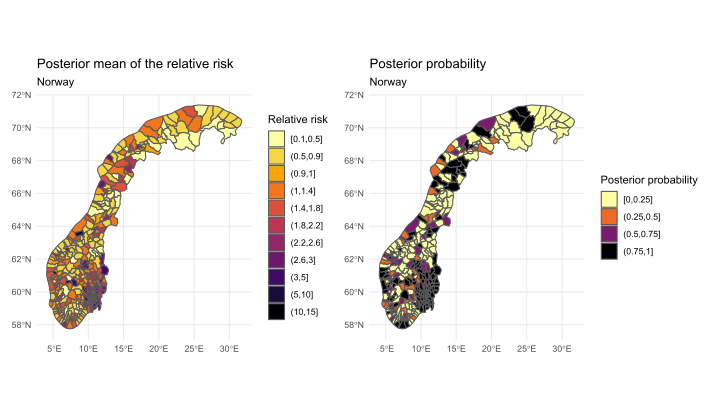
\includegraphics[width = \textwidth]{posterior_norway.png}
    \caption{Posterior mean of the area-specific risk and the posterior probability.}
    \label{posteriorNorway}
\end{figure}
% \begin{figure}[H]
%     \centering
%     \includesvg[width = textwidth]{posterior_norway.svg}
%     \caption{A negative binomial fit to the number of cases in Norwegian municipalities}
%     \label{nb_norge}
% \end{figure}
\clearpage
\section{Spatio-Temporal Models}
\subsection{Spatio-Temporal Models for Germany}
\subsection{Spatio-Temporal Models for Norway}
\section{Predictive Models}
\clearpage
\subsection{Predictive Models for Germany}
\subsection{Predictive Models for Norway}
% !TEX root = ../my-thesis.tex
%
\chapter{Further Analysis using R-Shiny}\label{ch:shiny}
R-Shiny is a framework that enables the creation of web applications and dashboards to visualize data interactively, to make statistics accessible to people without programming skills or a mathematical background, or to enable further analysis on research questions, to name just a few use cases. Dashboards have also been used by governments during the pandemic to effectively communicate infection data related to Covid-19, e.g. the Robert Koch Institute's Covid-19 Dashboard, which displays daily infection figures for each municipality in Germany that can be grouped by age group and gender, displays key figures such as the 7-day incidence and contains a choropleth map, among other features. The dashboard can be accessed at
\begin{center}
    \href{https://experience.arcgis.com/experience/478220a4c454480e823b17327b2bf1d4}{https://experience.arcgis.com/experience/478220a4c454480e823b17327b2bf1d4}
\end{center}
A similar dashboard is available for Norway and specifically for the municipality of Oslo:
\begin{center}
    \href{https://experience.arcgis.com/experience/742a281a0fa74ab79147a76e6b52833b}{https://experience.arcgis.com/experience/742a281a0fa74ab79147a76e6b52833b}
\end{center}
As part of this thesis, a dashboard was developed using the R-Shiny framework, with the intention to give the reader a bit more insight into the data. The dashboard comes with four main features:
\begin{itemize}
    \item[1.] The Data Explorer
    \item[2.] The SIR for Norway and Germany
    \item[3.] Spatial Modelling
    \item[4.] Temporal Modelling
\end{itemize}
\subsubsection*{The Data Explorer}
The main idea behind the data explorer is to display the data used to create all the models calculated in this work. The data can be visualized for Norway, Germany or Europe. Each tab contains a map and several drop-down menus where the user can select different things. For Norway and Germany, in addition to the variable to be displayed on the map, there is also the option to choose between three map types, hexagon maps, heat maps and choropleth maps. Hexagon maps can be seen as a mixture of a heat map and a histogram. Each bar represents the number of times a feature is present within a certain radius. The higher a bar is, the more often the feature is present. Figure~\ref{fig:map_1} shows the number of bakeries within a radius of 2.5 km. It is clear that most bakeries are found in Berlin and Munich.
\begin{figure}[H]
    \centering
    \includegraphics[width = \textwidth]{bakeries_germany_hex.png}
    \caption{A hexagon map of all bakeries in Germany.}
    \label{fig:map_1}
\end{figure}
The same information can also be conveyed using a heat map, as shown in Figure~\ref{fig:map_2}.
\begin{figure}[H]
    \centering
    \includegraphics[width = \textwidth]{bakeries_germany_heat.png}
    \caption{A heat map of all bakeries in Germany.}
    \label{fig:map_2}
\end{figure}
Through a choropleth map the number of bakeries in each municipality can be visualized, as seen in Figure~\ref{fig:map_3}.
\begin{figure}[H]
    \centering
    \includegraphics[width = \textwidth]{bakeries_germany_choro.png}
    \caption{A choropleth map of all bakeries in Germany.}
    \label{fig:map_3}
\end{figure}
The app also displays a histogram of the variable selected by the user. Finally, the user has the option to compare a municipality with the rest of the country in terms of indicators of Covid-19 severity. These indicators are the daily number of infections, the total number of infections and the seven-day incidence. This can be used to create charts like the one in Figure~\ref{fig:inc_muc}.
\begin{figure}[H]
    \centering
    \includegraphics[width = \textwidth]{inc_muc.png}
    \caption{The seven-day incidence in Munich compared to Germany.}
    \label{fig:inc_muc}
\end{figure}
For Europe, the user can view the features used in the calculation of the temporal models. The map can show mobility in different European countries, government measures and general key figures. The user can select a date to see, for example, which measurements were taken at Christmas 2020. Only a choropleth map is available here. Again, the user can view indicators of Covid-19 severity, this time comparing a country with the rest of Europe.
\subsubsection*{The SIR for Norway and Germany}
This is self-explanatory. The user can display the standardized incidence ratio either in Norway or in Germany.
\subsubsection*{Spatial Modelling}
Here the user can calculate his own BYM2 model, either for Norway or for Germany. Different variables can be selected to be added to the model, as well as values for $\sigma_0$ and $\alpha$, which are used for the PC prior. After pressing the button to calculate the model, which takes a few seconds, the map is updated and the user can now choose to display the relative risk, the posterior mean of the random effects, the exceedance probability or the spatial field. Two tables are also displayed. One containing all relevant performance measures and one containing all significant effects. Each time the user calculates a new model, new rows are added to the table. Via the ID column, the user can keep track of his models and see how the performance of a model changes or which effects turn out to be significant in which model.
\subsubsection*{Temporal Modelling}
This is the same as spatial modelling, but this time the user has the option to specify the type of temporal term to use, the country to use for modelling and the test size. The user can choose between five types of temporal terms:
\begin{itemize}
    \item[1.] An iid term
    \item[2.] A random walk of length 1
    \item[3.] A random walk of length 2
    \item[4.] An autoregressive process of order 1
    \item[5.] An Ornstein–Uhlenbeck process
\end{itemize}
33 countries can be selected for modelling and any number can be set for the test size. After the models have been calculated, two graphs are displayed. One for the predicted infection numbers in a country and one for the posterior temporal trend in that country. The graph for the predicted numbers includes a confidence interval for these predictions as well as the actual infection numbers in the country, an example of which can be seen in Figure~\ref{fig:sweden}.
\begin{figure}[H]
    \centering
    \includegraphics[width = \textwidth]{predicted_sweden.png}
    \caption{Predicted numbers in Sweden using an ar1 model with a test size of 28.}
    \label{fig:sweden}
\end{figure}
The same tables used in the Spatial Modelling tab are also used here and contain the same functionality. \\
The dashboard can be accessed via the following IP address:
\begin{center}
    \href{http://194.163.140.89:3838/}{http://194.163.140.89:3838/}
\end{center}
% !TEX root = ../my-thesis.tex
%
\chapter{Discussion}\label{sec:discussion}
After the models have been calculated, the next step is to critically examine and evaluate the results. The evaluation of the spatial models follows a simple scheme. First, a brief look is taken at the models without the spatial component, before the spatial models are reviewed and compared with the non-spatial models. Next, it is examined which factors significantly influence the risk of infection and why these factors might have an impact. For this, the coefficient of the BYM2 model are analysed. Finally, a look at area-specific risk is taken to see which regions in a given country are most at risk.
\section{Discussion of the (Non)-Spatial Models}
\subsection{Discussion of the (Non)-Spatial Models for Norway}\label{sec:models_norway}
The non-spatial model for Norway identified five significant effects:
\begin{itemize}
    \item The number of unemployed immigrants 
    \item The total number of immigrants 
    \item The urban density 
    \item The number of aerodromes 
    \item The proportion of females 
\end{itemize}
Moreover, the intercept was significant. \\
Comparing the spatial models with the non-spatial models using Table~\ref{allNorway}, it can be seen that BYM2, Besag and the non-spatial model performed almost equally well in terms of the DIC and WAIC, while the Leroux model performed best in terms of these two metrics. In terms of CPO, all spatial models performed better than the non-spatial model, with the Leroux model again performing best. However, the MAE shows that the non-spatial model has the best predictive performance, ahead of the Besag model, the BYM2 model and the Leroux model. This shows that the Leroux model overfits the training data more than the other models, a characteristic that can also be seen in Figure~\ref{comparison_norway_1} and Figure~\ref{comparison_norway_2}. The fact that the non-spatial model performs better than the spatial models is an indication that the spatial effect in Norway is not strong and that a different class of models may be better suited to identify critical factors affecting infection rates. Table~\ref{fixedAllNorway_spatial} also shows that adding the spatial effect did not suddenly cause any variables to become significant, while all variables, including the intercept, that were significant in the non-spatial model remained significant. Nevertheless, significant effects were found and have to be discussed. \\
The exponentiated intercept implies a risk rate of -60.8\% across Norway. The factor that influences the relative risk most is urban density, where an increase of 1 standard deviation leads to an increase in the relative risk of 22.5\%. The relationship between a higher number of residential buildings in a given area and the number of infections is probably due to the fact that with an increasing number of residential buildings comes an increasing number of inhabitants. A look at the Bravais-Pearson correlation coefficient confirms this assumption with $\rho=0.7070$. Furthermore, the correlation between urban density and population density is $0.8037$. This is convenient since studies analysing the relationship between urban density and Covid-19 usually define urban density as the number of inhabitants per square kilometre. Because of the positive relationship between urban density and population density, urban density acts as a proxy for population density in these models, so the relationship between higher population density and higher case numbers should also account for the higher infection rates in areas with higher urban density. According to Jamshidi et al. (2020) and Whittle \& Diaz-Artiles (2020), higher urban/population density and higher infection numbers are due to a decrease in proximity between people and an increase in the likelihood of interpersonal contact (Jamshidi2020global, Whittle2020ecological). Sigler et al. (2020) also found that dense urban environments provide more opportunities for the virus to spread, but that higher density had a stronger effect earlier and decreased in strength and importance over time\autocite[][]{sigler2020socio}. \\
Factors related to immigration also play a crucial role in the relative risk of developing Covid-19. A one standard deviation increase in the number of unemployed immigrants leads to a 20.8\% increase in risk and a one standard deviation increase in the total number of immigrants leads to a 20.3\% increase in risk. Unfortunately, there are no studies analysing the relationship between unemployed immigrants and the risk of developing Covid-19, as studies mostly focus on the relationship between unemployment in general and the risk of disease. Unemployment, however, turned out to be non-significant in the BYM2 model. Looking at older studies, Elkeles and Seifert (1996) conducted a longitudinal study that looked at the unemployment status and health of labour migrants in Germany. They found that immigrants were often employed in jobs with higher health risks and stress and therefore had poorer health \autocite[][]{elkeles1996immigrants}. Sia et al. (2019) analysed the association between immigration status and unemployment and men's and women's health using data from the Canadian Health Measures Survey. The study provided evidence of biological associations between unemployment and the likelihood of common chronic diseases, inflammation and possible malnutrition, with unemployed immigrants, and particularly unemployed immigrant women, being more prone to chronic diseases \autocite[][]{sia2019chronic}. Thus, there is precedent for an association between unemployment and immigrants and a higher risk of disease, however, further research would need to be conducted to analyse the association between unemployed immigrants and the risk of Covid-19 infection. \\
A higher risk among immigrants in Norway was already found in a study by Indseth et al. (2020). The reasons given are barriers to adequate information due to low health literacy in certain groups and misconceptions about Covid-19 or test criteria, as well as other socio-economic and environmental factors \autocite[][]{indseth2020covid}. Therefore, the results of the BYM2 model are consistent with this study. \\
Looking at the factors that reduce the risk of infection for Covid-19, for airports, a 1 standard deviation increase leads to a 12.2\% reduction in risk and a 1 standard deviation increase in the proportion of women leads to an 18.2\% reduction in the risk of infection. Neither result is consistent with current research. Gaskin et al. (2021) found that counties in the United States closer to an airport have higher Covid-19 rates than counties further from an airport \autocite[][]{gaskin2021geographic}. Daon et al. (2020) found that different airports have different risks of being a source of an outbreak, especially airports in low- to middle-income countries \autocite[][]{daon2020estimating}. \\
Many studies have investigated the relationship between gender and Covid-19 and most come to the same conclusion. While the risk of infection is the same in men and women, men tend to experience a higher severity and mortality rate for Covid-19 compared to women \autocite[][]{mukherjee2021covid, gausman2020sex, spagnolo2020sex, kopel2020racial}. \\
A look at the relative risk of infection in Figure~\ref{rr_norway} shows that the relative risk is below 1 in most of Norway, which is not too surprising considering that Norway has managed the pandemic quite well so far. The two municipalities with the highest relative risk are Iveland and Ålesund. However, a look at the posterior probability in Figure~\ref{posterior_norway} shows that the posterior probability of the risk being greater than 1 is less than 0.5 for Ålesund (0.47) and less than 0.75 for Iveland (0.62). Looking at the log posterior mean of the random effects, there is an increased risk in the regions around Oslo and in large parts of southern and central Norway, while the risk tends to be lower in the northern parts of the country.
\begin{figure}[H]
  \centering
  \includegraphics[width = \textwidth]{relative_risk_norway.png}
  \caption{Relative risk of contracting Covid-19 in Norway.}
  \label{rr_norway}
\end{figure}
\begin{figure}[H]
  \centering
  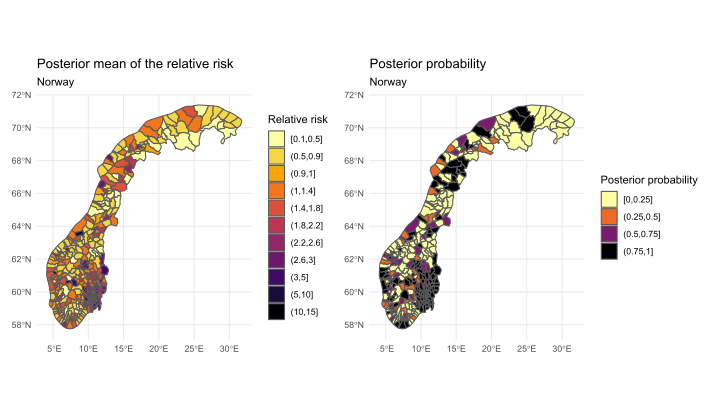
\includegraphics[width = \textwidth]{posterior_norway.png}
  \caption{Posterior mean of the municipality-specific relative risks $\zeta=\exp{\left(\xi\right)}$ compared with the whole of Norway (left) and posterior probability $\mathbb{P}\left(\zeta_i>1|\pmb{y}\right)$}
  \label{posterior_norway}
\end{figure}
\subsection{Discussion of the (Non)-Spatial Models for Germany}
In the non-spatial model for Germany, six coefficients were significant, in addition to the intercept:
\begin{itemize}
    \item The percentage of the vote for the right-wing populist AfD
    \item The population density
    \item The logarithmic trade tax
    \item The percentage of the vote for the SPD
    \item The percentage of the vote for the left-wing party "Die Linke"
    \item The percentage of the vote for the Green party
\end{itemize}
A look at Table~\ref{allGermany} shows that the spatial models outperform the non-spatial model in terms of the DIC and the WAIC, while all models perform about equally well in terms of the CPO. The predictive performance was best for the BYM2 model, just ahead of the Besag model, as indicated by the lowest values for the MAE. When adding the spatial term for the BYM2 model, several variables lose their significance, namely the percentage of the vote for the SPD, "Die Linke" and the Greens, while the intercept, the percentage of the vote for the AfD, population density and the logarithmic trade tax remain significant. \\
The exponentiated intercept implies a risk rate of -6.8\% across Germany. The greatest influence on the relative risk was determined to be the percentage of the vote for the far-right AfD. An increase in this variable by 1 standard deviation leads to an increase in the relative risk by 24.8\%. The AfD openly criticises the measures taken by the government in Germany to prevent the spread of Covid-19, which leads to a large proportion of the party's voters not taking the measures seriously and refusing to keep a safe distance or wear a mask in public spaces. Several studies have taken a look at the response of right-wing parties to the pandemic and how people who vote for these types of parties have reacted. Wondreys and Mudde (2020) point out that these parties were quick to warn about the virus, but once cases spiked, they criticised the measures taken to contain the spread of the virus. They also noted that right-wing parties often rejected the measures proposed by the leading parties because they themselves were part of the opposition \autocite[][]{wondreys2020victims}, as is the case with the AfD in Germany. Vieten (2020) shows how the far-right mobilises people for anti-hygiene or anti-lockdown protests and how this is used to normalise the global far-right \autocite[][]{vieten2020new}. Eberl et al. (2020) analysed data from the Austrian Corona Panel Project to test whether populism attitudes and belief in conspiracy theories related to Covid-19 are correlated. Using structural equation modelling, they show that populism indirectly influences Covid-19 conspiracy beliefs through trust in political and scientific institutions. They find that populist attitudes have a negative correlation with trust in the government and the parliament.Furthermore, they find that higher populist attitudes are negatively correlated with trust in science, a factor that reduces belief in Covid-19 conspiracy theories \autocite[][]{eberl2020populism}. Finally, Farias and Pilati (2020) conducted a study in Brazil to predict social distancing violation intention and past non-compliance during the Covid-19 pandemic, controlling for the effects of interolerence of insecurity and socio-demographic variables. Their results included that individuals who support right-wing parties are more likely to violate social distancing measures \autocite[][]{farias2020violating}. \\
An increase in population density by 1 standard deviation leads to a risk increase of 11.2\%. Reasons why a higher population density correlates positively with the number of infections have already been discussed in Section~\ref{sec:models_norway}. \\
The last significant effect is the logarithmic trade tax with an increase of 1 standard deviation leading to a 6.7\% increase in risk. There are no studies that specifically analyse the relationship between the trade tax and the risk of infection, but some studies have analysed infection rates in different spatial areas while controlling for factors such as income. In general, a negative relationship was found between areas with higher income and infection rates, meaning that areas with higher income had fewer cases of Covid-19. Cordes and Castro (2020) found that postcode areas in New York City with a low proportion of positive tests had higher incomes and also tested less compared to lower income areas. They also found that people in lower income areas were more likely to be without health insurance \autocite[][]{cordes2020spatial}. Coven and Gupta (2020) found that New York City residents who come from wealthier neighbourhoods are more likely to flee the city, and that people who live in low-income neighbourhoods are more likely to have frontline occupations and visit retail shops more often, increasing their exposure to Covid-19 \autocite[][]{coven2020disparities}. The situation seems to be the same in Europe, as Baena et al. (2020) found that districts in Barcelona with a lower average income had a higher Covid-19 incidence. They found that the incidence in the district with the lowest income was 2.5 times higher than in the district with the highest income \autocite[][]{baena2020impact}. Again, the results of the BYM2 model are not consistent with current research. \\
The relative risk of infection shown in Figure~\ref{rr_germany} is highest in eastern Germany, more specifically in the federal state of Saxony. Saxony has established itself as the political stronghold of the AfD in recent years, which has even led to the ruling party, the Union, moving further to the right on the political spectrum. In addition to Saxony, the traditionally highly conservative Bavaria and the populous Ruhr region also have a relative risk of over 1. Figure~\ref{posterior_germany} shows that for most of these regions the posterior mean of the random effects is also over 1, mostly with a posterior probability of at least 0.75.
\begin{figure}[H]
  \centering
  \includegraphics[width = \textwidth]{relative_risk_germany.png}
  \caption{Relative risk of contracting Covid-19 in Germany.}
  \label{rr_germany}
\end{figure}
\begin{figure}[H]
  \centering
  \includegraphics[width = \textwidth]{posterior_germany.png}
  \caption{Posterior mean of the municipality-specific relative risks $\zeta=\exp{\left(\xi\right)}$ compared with the whole of Germany (left) and posterior probability $\mathbb{P}\left(\zeta_i>1|\pmb{y}\right)$}
  \label{posterior_germany}
\end{figure}
% !TEX root = ../my-thesis.tex
%
\chapter{Conclusion}\label{sec:conclussion}
The aim of this work was to identify factors that have a significant impact on the current Covid-19 infection numbers in Germany and Norway using both a Bayesian approach that takes into account the spatial neighbourhood structure of each country and a non-Bayesian machine learning approach, and to compare these approaches to see which one proves more useful for this type of analysis. Another goal was to determine factors influencing infection numbers over time, namely government actions in response to the pandemic, changes in population mobility patterns, and the prevalence of different strains of Covid-19. \\
Based on the analysis of the differences between the spatial Bayesian and the non-Bayesian models for which no temporal effect is used, it can be concluded that the use of the Bayesian model with inclusion of a spatial term showed superior performance in terms of the mean absolute error, both in training and in testing. This was observed for Germany and for Norway. \\
For Germany, the factors that have a significant impact on the prevalence of Covid-19 are population density, the percentage of votes for the right-wing party AfD and the logarithmic trade tax. All three factors had a positive effect on the predicted infection rates, with current research clearly supporting the link between population density and infection rates, as well as the link between right-wing parties and the tendency for people who support these parties to be at higher risk of infection due to not following Covid-19 guidelines. On the other hand, recent research suggests that people living in higher income or richer regions have a lower risk of infection, while the opposite is suggested by the model calculated for Germany. \\
For Norway, these factors are urban density, the number of unemployed immigrants in a municipality, the total number of immigrants in a municipality and the proportion of women. The proportion of women is the only effect where a negative influence on the predicted infection numbers is observed. However, this association is not supported by current research which suggests that men and women are equally likely to contract Covid-19. No research has yet been conducted to analyse the association between unemployed immigrants and the risk of Covid-19, which makes it difficult to evaluate this effect as there is no research to compare it to. The association between immigrants in Norway and the risk of infection with Covid-19, as well as the association between the risk of infection and urban density, is consistent with current research which suggests that immigrants in Norway have a higher risk of infection and that higher density in urban areas leads to a higher risk of infection. \\
Temporal modelling proved more difficult, with no distribution fitting the data reasonably well for Germany or Norway. A small test size limited the interpretation of the results. For both countries, the only significant effect on infection rates found was mobility in workplaces with a higher workplace mobility leading to a higher risk of infection. This is in line with current research. \\
Based on these conclusions, people living in areas with characteristics such as a higher proportion of people voting for right-wing parties or a higher population or urban density should be cautious in their daily lives and keep a safe distance from other people to limit their risk of contracting Covid-19. \\
Further research is needed to determine the relationship between areas in Germany that have a higher logarithmic trade tax and the risk of contracting Covid-19 in these areas. Research can never take all factors into account. Therefore, the association between these two variables could possibly be explained by a third variable. The same applies to the association between the proportion of women in a Norwegian municipality and the risk of contracting Covid-19.  \\
Future research could analyse the spatio-temporal relationship between the risk of infection and various factors such as government measures. In addition to nationwide government measures, there are local government measures, both in Germany and Norway. Obtaining this data is a time-consuming task that would require manual collection of this data from official local government sources, as currently no comprehensive dataset exists for either country. Developing a spatio-temporal model based on the demographic and infrastructural variables used for the spatial models in this thesis, as well as the variables used for the temporal models, has the potential to lead to new insights into which factors are driving up infection rates and which measures are successful in preventing new infections. \\
In summary, this thesis has shown that a Bayesian approach that models the spatial neighbourhood structure in a country is superior to an approach where no spatial neighbourhood structure is modelled. Furthermore, several factors were found to positively influence the risk of Covid-19 infection, both in Germany and Norway, and are supported by current research.
% !TEX root = ../my-thesis.tex
%
\chapter{Appendix}
\label{sec:appendix}
\section{Probability Distributions}
\subsection{The Normal Distribution}
The normal distribution is an important type of continuous probability distribution in stochastics. The special significance of the normal distribution is based, among other things, on the central limit theorem, according to which distributions that result from the additive combination of a large number of independent influences are approximately normally distributed under weak conditions. \\
The density is given by
\begin{equation}
    f\left(\pmb{x}|\mu,\sigma\right)=\frac{1}{\sigma\sqrt{2\pi}}\exp\left(-\frac{1}{2}\left(\frac{\pmb{x}-\mu}{\sigma}\right)^2\right).
\end{equation}
The first two moments of the distribution are given by
\begin{align}
    \mathbb{E}\left[X\right] &= \mu \\
    \hbox{Var}\left[X\right] &= \sigma^2.
\end{align}
The graph of this density function has a "bell-shaped form" and is symmetrical with $\mu$ as the centre of symmetry \autocite[][83-85]{fahrmeir2016statistik}.
\subsection{The Poisson Distribution}
The Poisson distribution is a discrete probability distribution that can be used to model the number of events that occur independently of each other at a constant mean rate in a fixed time interval or spatial area. \\
The density is given by
\begin{equation}
    f\left(k\right)=\mathbb{P}\left(X=k\right)=\begin{cases}
    \frac{\lambda^k}{k!}\exp\left(-\lambda\right) & \hbox{for }x\in\left\lbrace0,1,...\right\rbrace \\
    0 & \hbox{else}
    \end{cases}
\end{equation}
with $\lambda$ representing the expected value of $X$.  \\
The first two moments of the distribution are given by
\begin{align}
    \mathbb{E}\left[X\right] &= \lambda \label{eq:poisson_exp}\\
    \hbox{Var}\left[X\right] &= \lambda \label{eq:poisson_var}.
\end{align}
For $\lambda\geq10$ the distribution becomes approximately symmetrical and can thus be approximated by a normal distribution \autocite[][243]{fahrmeir2016statistik}.
\subsection{The Negative Binomial Distribution}
The negative binomial distribution is a univariate probability distribution that belongs to the discrete probability distributions. It models the number of trials required to achieve a given number of successes in a Bernoulli process. \\
The density is given by
\begin{equation}
    f\left(k,r,p\right)=\mathbb{P}\left(X=k\right)=\begin{pmatrix} k+r-1\\r-1\end{pmatrix}\left(1-p\right)^kp^r,
\end{equation}
with $r$ the number of successes, $k$ the number of failures, and $p$ the probability of success. \\
The first two moments of the distribution are given by
\begin{align}
    \mathbb{E}\left[X\right] &= \frac{pr}{1-p} \\
    \hbox{Var}\left[X\right] &= \frac{pr}{\left(1-p\right)^2}.
\end{align} 
For large values of $r$, the negative binomial distribution can be approximated by a normal distribution
\cite{haldane1941fitting}.
\clearpage
\section{Distribution Fits}
\subsection{Distribution Fits for Germany}
% \begin{figure}[H]
%     \centering
%     \includesvg[width = 0.8\textwidth]{fit_normal_germany.svg}
%     \caption{A normal fit to the number of cases in German municipalities}
%     \label{fitNormalGermany}
% \end{figure}
\begin{figure}[H]
    \centering
    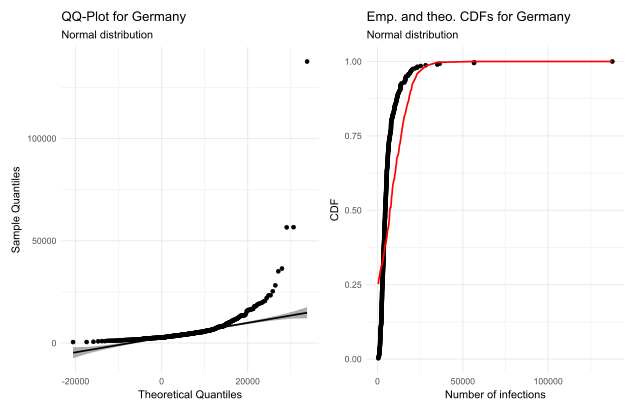
\includegraphics[width = 0.8\textwidth]{fit_normal_germany.png}
    \caption{A normal fit to the number of cases in German municipalities}
    \label{fitNormalGermany}
\end{figure}
% \begin{figure}[H]
%     \centering
%     \includesvg[width = 0.8\textwidth]{fit_poisson_germany.svg}
%     \caption{A Poisson fit to the number of cases in German municipalities}
%     \label{fitPoissonGermany}
% \end{figure}
\begin{figure}[H]
    \centering
    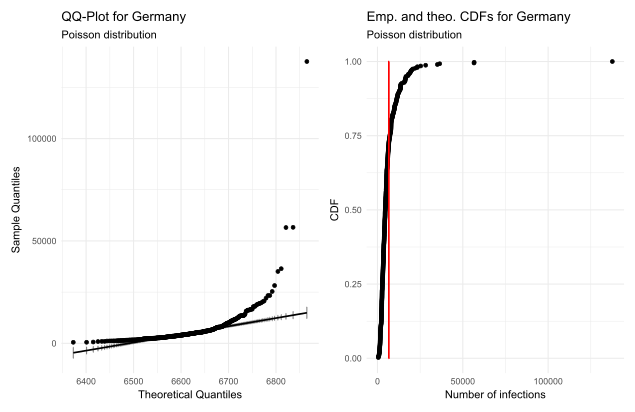
\includegraphics[width = 0.8\textwidth]{fit_poisson_germany.png}
    \caption{A Poisson fit to the number of cases in German municipalities}
    \label{fitPoissonGermany}
\end{figure}
\subsection{Distribution Fits for Norway}
% \begin{figure}[H]
%     \centering
%     \includesvg[width = 0.8\textwidth]{fit_normal_norway.svg}
%     \caption{A normal fit to the number of cases in Norwegian municipalities}
%     \label{fitNormalNorway
% \end{figure}
\begin{figure}[H]
    \centering
    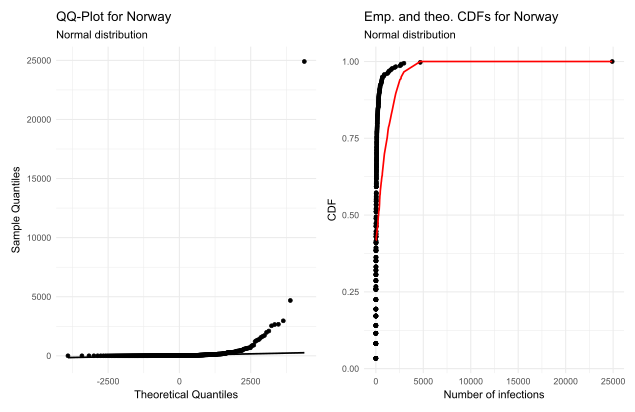
\includegraphics[width = 0.8\textwidth]{fit_normal_norway.png}
    \caption{A normal fit to the number of cases in Norwegian municipalities}
    \label{fitNormalNorway}
\end{figure}
% \begin{figure}[H]
%     \centering
%     \includesvg[width = 0.8\textwidth]{fit_poisson_norway.svg}
%     \caption{A Poisson fit to the number of cases in Norwegian municipalities}
%     \label{fitPoissonNorway}
% \end{figure}
\begin{figure}[H]
    \centering
    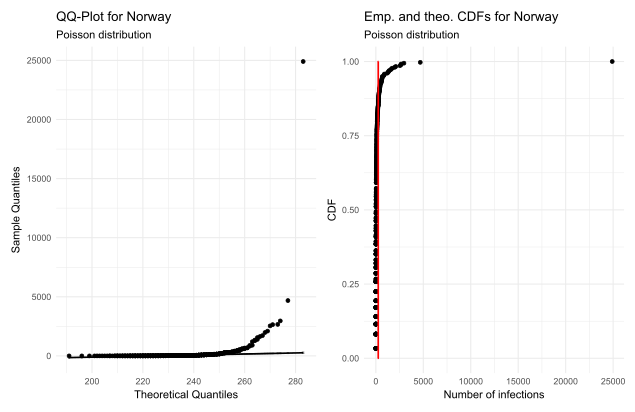
\includegraphics[width = 0.8\textwidth]{fit_poisson_norway.png}
    \caption{A Poisson fit to the number of cases in Norwegian municipalities}
    \label{fitPoissonNorway}
\end{figure}
\clearpage
\section{Prior Sensitivity for Germany}
\begin{figure}[H]
    \centering
    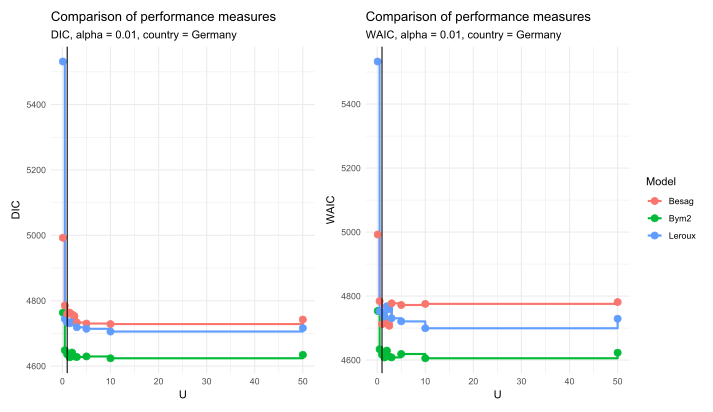
\includegraphics[width = \textwidth]{comparison_1_germany.png}
    \caption{Value of the DIC and WAIC when changing the value for $\sigma_0$. The black line highlights the values for $\sigma_0$ = 1.}
    \label{comparison_germany_1}
\end{figure}
% \begin{figure}[H]
%     \centering
%     \includesvg[width = \textwidth]{comparison_1_germany.svg}
%     \caption{Value of the DIC and WAIC when changing the value for $\sigma_0$. The black line highlights the values for $\sigma_0$ = 1.}
%     \label{comparison_germany_1}
% \end{figure}
\begin{figure}[H]
    \centering
    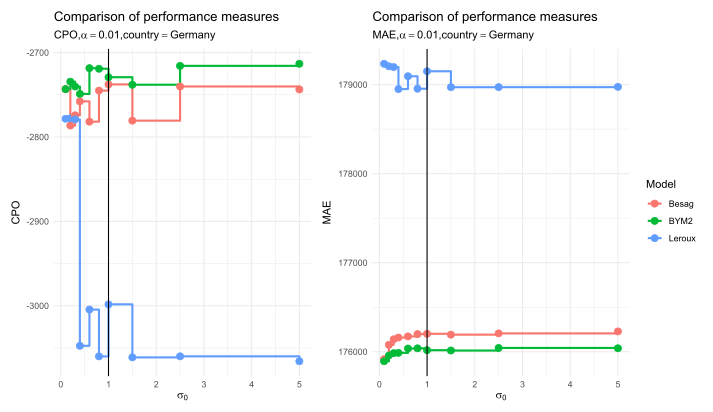
\includegraphics[width = \textwidth]{comparison_2_germany.png}
    \caption{Value of the CPO and MAE when changing the value for $\sigma_0$. The black line highlights the values for $\sigma_0$ = 1.}
    \label{comparison_germany_2}
\end{figure}
% \begin{figure}[H]
%     \centering
%     \includesvg[width = \textwidth]{comparison_2_germany.svg}
%     \caption{Value of the CPO and MAE when changing the value for $\sigma_0$. The black line highlights the values for $\sigma_0$ = 1.}
%     \label{comparison_germany_2}
% \end{figure}
\section{Code Examples}
\subsection{Specifying the Different Types of Models}
\begin{lstlisting}[caption={Specifying different models in INLA.}, label={codeModels}, language=R]
# set the seed
set.seed(420)
# draw a sample
test <- sample(
    seq_len(nrow(newest_numbers)),
    size = floor(0.2 * nrow(newest_numbers))
  )
# get the number of infections for the test data
test_value <- newest_numbers$value[test]
# set the number of infections to NA in the train data
newest_numbers$value[test] <- NA
# define the link function
link <- rep(NA, nrow(newest_numbers))
link[which(is.na(newest_numbers$value))] <- 1
# define the penalised prior
prior_1 <- list(
  prec = list(
    prior = "pc.prec",
    param = c(1, 0.01)
  )
)
# create the neighbordhood matrix
nb <- poly2nb(newest_numbers)
# save the matrix
nb2INLA("maps/map.adj", nb)
g <- inla.read.graph(filename = "maps/map.adj")
# define the C matrix for the Leroux model
Q <- Diagonal(x = sapply(nb, length))
for (i in 2:nrow(newest_numbers)) {
  Q[i - 1, i] <- -1
  Q[i, i - 1] <- -1
}

C <- Diagonal(x = 1, n = nrow(newest_numbers)) - Q
# define the formula for besags proper model
formula_besag <- value ~
  pop_dens + urb_dens + sex +
  f(idarea_1, model = "besagproper", graph = g, hyper = prior_1)
# define the formula for bym2 model
formula_bym2 <- value ~
  pop_dens + urb_dens + sex +
  f(
    idarea_1, model = "bym2", graph = g,
    scale.model = TRUE, hyper = prior_1
  )
# define the formula for leroux model
formula_leroux <- value ~
  pop_dens + urb_dens + sex +
  f(idarea_1, model = "generic1", Cmatrix = C, hyper = prior_1)
# compute the models
res_besag <- inla(
  formula_besag,
  family = "nbinomial",
  data = newest_numbers,
  E = expected_count,
  control.predictor = list(
    compute = TRUE,
    link = link
  ),
  Ntrials = newest_numbers$population,
  control.compute = list(dic = TRUE, waic = TRUE, cpo = TRUE)
)
res_bym2 <- inla(
  formula_bym2,
  family = "nbinomial",
  data = newest_numbers,
  E = expected_count,
  control.predictor = list(
    compute = TRUE,
    link = link
  ),
  Ntrials = newest_numbers$population,
  control.compute = list(dic = TRUE, waic = TRUE, cpo = TRUE)
)
res_leroux <- inla(
  formula_leroux,
  family = "nbinomial",
  data = newest_numbers,
  E = expected_count,
  control.predictor = list(
    compute = TRUE,
    link = link
  ),
  Ntrials = newest_numbers$population,
  control.compute = list(dic = TRUE, waic = TRUE, cpo = TRUE)
)
\end{lstlisting}
\subsection{Making Predictions for the Test Data}
\begin{lstlisting}[caption={The code for making predictions in INLA.}, label={codePrediction}, language=R]
# create a vector to save the predictions to
predicted <- c()
# now make the predictions
for(i in seq_len(nrow(newest_numbers))) {
  predicted[i] <- inla.emarginal(
    function(x) x * newest_numbers$population[i],
    res_bym2$marginals.fitted.values[[i]]
  )
}
# calculate the MAE for the test data
mean(abs(predicted[test] - test))

\end{lstlisting}
% \subsection{Variable Selection using INLA}
% \begin{lstlisting}[caption={The code for variable selection in INLA.}, label={codeSelection}, language=R]
% # define the stack
% stack_all <- inla.stack(
%   data = list(value = newest_numbers$value),
%   A = list(1),
%   effects = list(
%     data.frame(
%       Intercept = 1,
%       newest_numbers[, c(2:15, 20:35, 43:46)]
%     )
%   )
% )
% # run backwards varaible selection
% result_all_backwards <- INLAstep(
%   fam1 = "nbinomial",
%   newest_numbers,
%   in_stack = stack_all,
%   invariant = "Intercept",
%   direction = "backwards",
%   include = c(2:15, 20:35, 43:46),
%   y = "value",
%   y2 = "value",
%   powerl = 1,
%   inter = 1,
%   thresh = 2,
%   num.threads = 7
% )
% # run forwards variable selection
% result_all_forwards <- INLAstep(
%   fam1 = "nbinomial",
%   newest_numbers,
%   in_stack = stack_all,
%   invariant = "Intercept",
%   direction = "forwards",
%   include = c(2:15, 20:35, 43:46),
%   y = "value",
%   y2 = "value",
%   powerl = 1,
%   inter = 1,
%   thresh = 2,
%   num.threads = 7
% )
% \end{lstlisting}
\subsection{Calculating the Posterior Mean}
\begin{lstlisting}[caption={Calculating the posterior mean of a coefficent.}, label={codePosteriorMean}, language=R]
inla.emarginal(exp, model_leroux$marginals.fixed$trade_tax)
# calculate the increase in risk for an increase 
# by 2 in the trade tax
inla.emarginal(
  exp,
  model_leroux$marginals.fixed$trade_tax
  ) ^ 2
\end{lstlisting}
\subsection{Calculating a Credibility Interval}
\begin{lstlisting}[caption={Extracting the credibility interval for a coefficient}, label={codeCredibility}, language=R]
inla.qmarginal(
  c(0.025,0.975),
  inla.tmarginal(
    exp,
    model_leroux$marginals.fixed$trade_tax
  )
)
\end{lstlisting}
\subsection{Best Spatial Models For Germany}
\subsubsection{Best Spatial Model using Demographic Variables}
\begin{lstlisting}[caption={The code for the demographic model.}, label={codeDemoGermany}, language=R]
prior_1 <- list(
  prec = list(
    prior = "pc.prec",
    param = c(1, 0.01)
  )
)
formula <- value ~
  pop_dens + urb_dens + SPD + Gruene + FDP + die_linke +
  f(
    idarea_1, model = "bym2", graph = g,
    scale.model = TRUE, hyper = prior_1
  )
\end{lstlisting}
\subsubsection{Best Spatial Model using Infrastructural Variables}
\begin{lstlisting}[caption={The code for the infrastructure model.}, label={codeInfraGermany}, language=R]
prior_1 <- list(
  prec = list(
    prior = "pc.prec",
    param = c(1, 0.01)
  )
)
formula <- value ~
  pop_dens + urb_dens + clinic + place_of_worship + retail +
  nursing_home + aerodrome + platform + higher_education +
  f(
    idarea_1, model = "bym2", graph = g,
    scale.model = TRUE, hyper = prior_1
  )
\end{lstlisting}
\subsubsection{Best Spatial Model using Both Types of Variables}
\begin{lstlisting}[caption={The code for the demographic + infrastructure model.}, label={codeBothGermany}, language=R]
prior_1 <- list(
  prec = list(
    prior = "pc.prec",
    param = c(1, 0.01)
  )
)
formula <- value ~
  pop_dens + urb_dens + sex + log(trade_tax) + SPD +
  Gruene + FDP + die_linke + clinic + place_of_worship +
  retail + nursing_home + aerodrome + platform +
  higher_education +
  f(
    idarea_1, model = "bym2", graph = g,
    scale.model = TRUE, hyper = prior_1
  )
\end{lstlisting}
\subsection{Best Spatial Models For Norway}
\subsubsection{Best Spatial Model using Demographic Variables}
\begin{lstlisting}[caption={The code for the demographic model.}, label={codeDemoNorway}, language = R]
prior_1 <- list(
  prec = list(
    prior = "pc.prec",
    param = c(0.5 / 0.31, 0.01)
  )
)
formula <- value ~
  urb_dens + sex +
  f(
    idarea_1, model = "bym2", graph = g,
    scale.model = TRUE, hyper = prior_1
  )
\end{lstlisting}
\subsubsection{Best Spatial Model using Infrastructural Variables}
\begin{lstlisting}[caption={The code for the infrastructural model.}, label={codeInfraNorway}, language = R]
prior_1 <- list(
  prec = list(
    prior = "pc.prec",
    param = c(0.5 / 0.31, 0.01)
  )
)
formula <- value ~
  urb_dens + marketplace + place_of_worship +
  nursing_home + aerodrome + office + platform +
  higher_education +
  f(
    idarea_1, model = "bym2", graph = g,
    scale.model = TRUE, hyper = prior_1
  )
\end{lstlisting}
\subsubsection{Best Spatial Model using Both Types of Variables}
\begin{lstlisting}[caption={The code for the demographic + infrastructure model.}, label={codeBothNorway}, language=R]
prior_1 <- list(
  prec = list(
    prior = "pc.prec",
    param = c(0.5 / 0.31, 0.01)
  )
)
formula <- value ~
  urb_dens + median_age + unemp_tot + unemp_immg +
  immigrants_total + sex + marketplace + place_of_worship + 
  nursing_home + aerodrome + office + platform +
  higher_education +
  f(
    idarea_1, model = "bym2", graph = g,
    scale.model = TRUE, hyper = prior_1
  )
\end{lstlisting}
\clearpage

{%
\setstretch{1.1}
\renewcommand{\bibfont}{\normalfont\small}
\setlength{\biblabelsep}{0pt}
\setlength{\bibitemsep}{0.5\baselineskip plus 0.5\baselineskip}
\printbibliography[nottype=online]
\newrefcontext[labelprefix={@}]
\printbibliography[heading=subbibliography,title={Webpages},type=online]
}
\cleardoublepage

%\lstlistoflistings
\cleardoublepage

\appendix\cleardoublepage
%% !TEX root = ../my-thesis.tex
%
\chapter{Appendix}
\label{sec:appendix}
\section{Probability Distributions}
\subsection{The Normal Distribution}
The normal distribution is an important type of continuous probability distribution in stochastics. The special significance of the normal distribution is based, among other things, on the central limit theorem, according to which distributions that result from the additive combination of a large number of independent influences are approximately normally distributed under weak conditions. \\
The density is given by
\begin{equation}
    f\left(\pmb{x}|\mu,\sigma\right)=\frac{1}{\sigma\sqrt{2\pi}}\exp\left(-\frac{1}{2}\left(\frac{\pmb{x}-\mu}{\sigma}\right)^2\right).
\end{equation}
The first two moments of the distribution are given by
\begin{align}
    \mathbb{E}\left[X\right] &= \mu \\
    \hbox{Var}\left[X\right] &= \sigma^2.
\end{align}
The graph of this density function has a "bell-shaped form" and is symmetrical with $\mu$ as the centre of symmetry \autocite[][83-85]{fahrmeir2016statistik}.
\subsection{The Poisson Distribution}
The Poisson distribution is a discrete probability distribution that can be used to model the number of events that occur independently of each other at a constant mean rate in a fixed time interval or spatial area. \\
The density is given by
\begin{equation}
    f\left(k\right)=\mathbb{P}\left(X=k\right)=\begin{cases}
    \frac{\lambda^k}{k!}\exp\left(-\lambda\right) & \hbox{for }x\in\left\lbrace0,1,...\right\rbrace \\
    0 & \hbox{else}
    \end{cases}
\end{equation}
with $\lambda$ representing the expected value of $X$.  \\
The first two moments of the distribution are given by
\begin{align}
    \mathbb{E}\left[X\right] &= \lambda \label{eq:poisson_exp}\\
    \hbox{Var}\left[X\right] &= \lambda \label{eq:poisson_var}.
\end{align}
For $\lambda\geq10$ the distribution becomes approximately symmetrical and can thus be approximated by a normal distribution \autocite[][243]{fahrmeir2016statistik}.
\subsection{The Negative Binomial Distribution}
The negative binomial distribution is a univariate probability distribution that belongs to the discrete probability distributions. It models the number of trials required to achieve a given number of successes in a Bernoulli process. \\
The density is given by
\begin{equation}
    f\left(k,r,p\right)=\mathbb{P}\left(X=k\right)=\begin{pmatrix} k+r-1\\r-1\end{pmatrix}\left(1-p\right)^kp^r,
\end{equation}
with $r$ the number of successes, $k$ the number of failures, and $p$ the probability of success. \\
The first two moments of the distribution are given by
\begin{align}
    \mathbb{E}\left[X\right] &= \frac{pr}{1-p} \\
    \hbox{Var}\left[X\right] &= \frac{pr}{\left(1-p\right)^2}.
\end{align} 
For large values of $r$, the negative binomial distribution can be approximated by a normal distribution
\cite{haldane1941fitting}.
\clearpage
\section{Distribution Fits}
\subsection{Distribution Fits for Germany}
% \begin{figure}[H]
%     \centering
%     \includesvg[width = 0.8\textwidth]{fit_normal_germany.svg}
%     \caption{A normal fit to the number of cases in German municipalities}
%     \label{fitNormalGermany}
% \end{figure}
\begin{figure}[H]
    \centering
    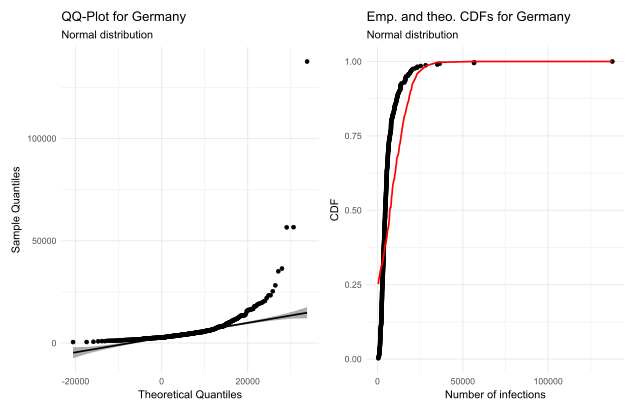
\includegraphics[width = 0.8\textwidth]{fit_normal_germany.png}
    \caption{A normal fit to the number of cases in German municipalities}
    \label{fitNormalGermany}
\end{figure}
% \begin{figure}[H]
%     \centering
%     \includesvg[width = 0.8\textwidth]{fit_poisson_germany.svg}
%     \caption{A Poisson fit to the number of cases in German municipalities}
%     \label{fitPoissonGermany}
% \end{figure}
\begin{figure}[H]
    \centering
    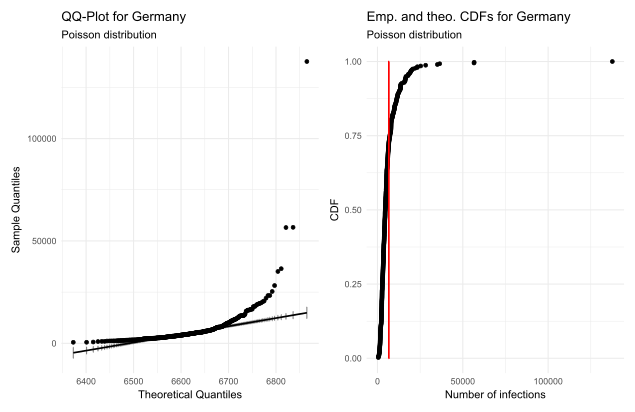
\includegraphics[width = 0.8\textwidth]{fit_poisson_germany.png}
    \caption{A Poisson fit to the number of cases in German municipalities}
    \label{fitPoissonGermany}
\end{figure}
\subsection{Distribution Fits for Norway}
% \begin{figure}[H]
%     \centering
%     \includesvg[width = 0.8\textwidth]{fit_normal_norway.svg}
%     \caption{A normal fit to the number of cases in Norwegian municipalities}
%     \label{fitNormalNorway
% \end{figure}
\begin{figure}[H]
    \centering
    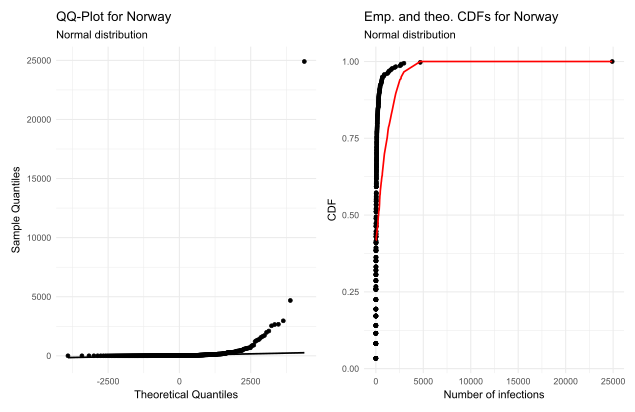
\includegraphics[width = 0.8\textwidth]{fit_normal_norway.png}
    \caption{A normal fit to the number of cases in Norwegian municipalities}
    \label{fitNormalNorway}
\end{figure}
% \begin{figure}[H]
%     \centering
%     \includesvg[width = 0.8\textwidth]{fit_poisson_norway.svg}
%     \caption{A Poisson fit to the number of cases in Norwegian municipalities}
%     \label{fitPoissonNorway}
% \end{figure}
\begin{figure}[H]
    \centering
    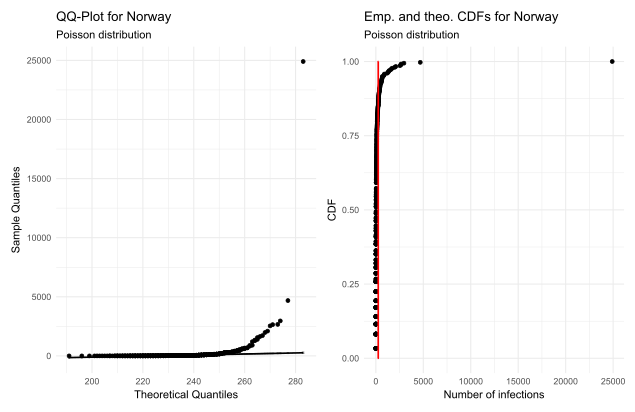
\includegraphics[width = 0.8\textwidth]{fit_poisson_norway.png}
    \caption{A Poisson fit to the number of cases in Norwegian municipalities}
    \label{fitPoissonNorway}
\end{figure}
\clearpage
\section{Prior Sensitivity for Germany}
\begin{figure}[H]
    \centering
    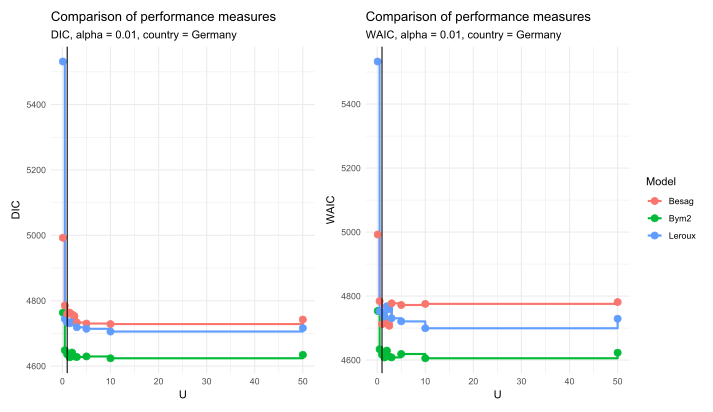
\includegraphics[width = \textwidth]{comparison_1_germany.png}
    \caption{Value of the DIC and WAIC when changing the value for $\sigma_0$. The black line highlights the values for $\sigma_0$ = 1.}
    \label{comparison_germany_1}
\end{figure}
% \begin{figure}[H]
%     \centering
%     \includesvg[width = \textwidth]{comparison_1_germany.svg}
%     \caption{Value of the DIC and WAIC when changing the value for $\sigma_0$. The black line highlights the values for $\sigma_0$ = 1.}
%     \label{comparison_germany_1}
% \end{figure}
\begin{figure}[H]
    \centering
    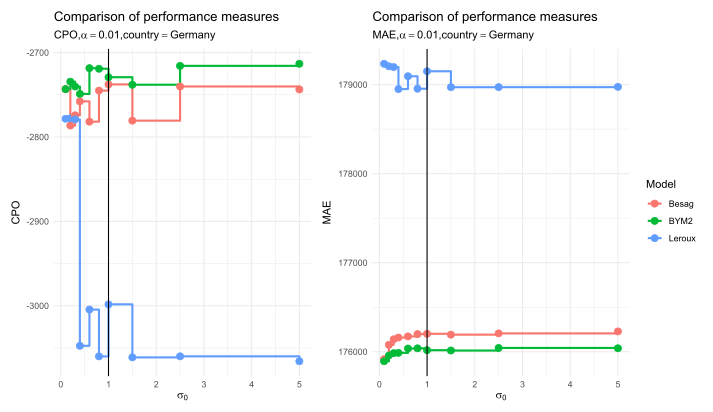
\includegraphics[width = \textwidth]{comparison_2_germany.png}
    \caption{Value of the CPO and MAE when changing the value for $\sigma_0$. The black line highlights the values for $\sigma_0$ = 1.}
    \label{comparison_germany_2}
\end{figure}
% \begin{figure}[H]
%     \centering
%     \includesvg[width = \textwidth]{comparison_2_germany.svg}
%     \caption{Value of the CPO and MAE when changing the value for $\sigma_0$. The black line highlights the values for $\sigma_0$ = 1.}
%     \label{comparison_germany_2}
% \end{figure}
\section{Code Examples}
\subsection{Specifying the Different Types of Models}
\begin{lstlisting}[caption={Specifying different models in INLA.}, label={codeModels}, language=R]
# set the seed
set.seed(420)
# draw a sample
test <- sample(
    seq_len(nrow(newest_numbers)),
    size = floor(0.2 * nrow(newest_numbers))
  )
# get the number of infections for the test data
test_value <- newest_numbers$value[test]
# set the number of infections to NA in the train data
newest_numbers$value[test] <- NA
# define the link function
link <- rep(NA, nrow(newest_numbers))
link[which(is.na(newest_numbers$value))] <- 1
# define the penalised prior
prior_1 <- list(
  prec = list(
    prior = "pc.prec",
    param = c(1, 0.01)
  )
)
# create the neighbordhood matrix
nb <- poly2nb(newest_numbers)
# save the matrix
nb2INLA("maps/map.adj", nb)
g <- inla.read.graph(filename = "maps/map.adj")
# define the C matrix for the Leroux model
Q <- Diagonal(x = sapply(nb, length))
for (i in 2:nrow(newest_numbers)) {
  Q[i - 1, i] <- -1
  Q[i, i - 1] <- -1
}

C <- Diagonal(x = 1, n = nrow(newest_numbers)) - Q
# define the formula for besags proper model
formula_besag <- value ~
  pop_dens + urb_dens + sex +
  f(idarea_1, model = "besagproper", graph = g, hyper = prior_1)
# define the formula for bym2 model
formula_bym2 <- value ~
  pop_dens + urb_dens + sex +
  f(
    idarea_1, model = "bym2", graph = g,
    scale.model = TRUE, hyper = prior_1
  )
# define the formula for leroux model
formula_leroux <- value ~
  pop_dens + urb_dens + sex +
  f(idarea_1, model = "generic1", Cmatrix = C, hyper = prior_1)
# compute the models
res_besag <- inla(
  formula_besag,
  family = "nbinomial",
  data = newest_numbers,
  E = expected_count,
  control.predictor = list(
    compute = TRUE,
    link = link
  ),
  Ntrials = newest_numbers$population,
  control.compute = list(dic = TRUE, waic = TRUE, cpo = TRUE)
)
res_bym2 <- inla(
  formula_bym2,
  family = "nbinomial",
  data = newest_numbers,
  E = expected_count,
  control.predictor = list(
    compute = TRUE,
    link = link
  ),
  Ntrials = newest_numbers$population,
  control.compute = list(dic = TRUE, waic = TRUE, cpo = TRUE)
)
res_leroux <- inla(
  formula_leroux,
  family = "nbinomial",
  data = newest_numbers,
  E = expected_count,
  control.predictor = list(
    compute = TRUE,
    link = link
  ),
  Ntrials = newest_numbers$population,
  control.compute = list(dic = TRUE, waic = TRUE, cpo = TRUE)
)
\end{lstlisting}
\subsection{Making Predictions for the Test Data}
\begin{lstlisting}[caption={The code for making predictions in INLA.}, label={codePrediction}, language=R]
# create a vector to save the predictions to
predicted <- c()
# now make the predictions
for(i in seq_len(nrow(newest_numbers))) {
  predicted[i] <- inla.emarginal(
    function(x) x * newest_numbers$population[i],
    res_bym2$marginals.fitted.values[[i]]
  )
}
# calculate the MAE for the test data
mean(abs(predicted[test] - test))

\end{lstlisting}
% \subsection{Variable Selection using INLA}
% \begin{lstlisting}[caption={The code for variable selection in INLA.}, label={codeSelection}, language=R]
% # define the stack
% stack_all <- inla.stack(
%   data = list(value = newest_numbers$value),
%   A = list(1),
%   effects = list(
%     data.frame(
%       Intercept = 1,
%       newest_numbers[, c(2:15, 20:35, 43:46)]
%     )
%   )
% )
% # run backwards varaible selection
% result_all_backwards <- INLAstep(
%   fam1 = "nbinomial",
%   newest_numbers,
%   in_stack = stack_all,
%   invariant = "Intercept",
%   direction = "backwards",
%   include = c(2:15, 20:35, 43:46),
%   y = "value",
%   y2 = "value",
%   powerl = 1,
%   inter = 1,
%   thresh = 2,
%   num.threads = 7
% )
% # run forwards variable selection
% result_all_forwards <- INLAstep(
%   fam1 = "nbinomial",
%   newest_numbers,
%   in_stack = stack_all,
%   invariant = "Intercept",
%   direction = "forwards",
%   include = c(2:15, 20:35, 43:46),
%   y = "value",
%   y2 = "value",
%   powerl = 1,
%   inter = 1,
%   thresh = 2,
%   num.threads = 7
% )
% \end{lstlisting}
\subsection{Calculating the Posterior Mean}
\begin{lstlisting}[caption={Calculating the posterior mean of a coefficent.}, label={codePosteriorMean}, language=R]
inla.emarginal(exp, model_leroux$marginals.fixed$trade_tax)
# calculate the increase in risk for an increase 
# by 2 in the trade tax
inla.emarginal(
  exp,
  model_leroux$marginals.fixed$trade_tax
  ) ^ 2
\end{lstlisting}
\subsection{Calculating a Credibility Interval}
\begin{lstlisting}[caption={Extracting the credibility interval for a coefficient}, label={codeCredibility}, language=R]
inla.qmarginal(
  c(0.025,0.975),
  inla.tmarginal(
    exp,
    model_leroux$marginals.fixed$trade_tax
  )
)
\end{lstlisting}
\subsection{Best Spatial Models For Germany}
\subsubsection{Best Spatial Model using Demographic Variables}
\begin{lstlisting}[caption={The code for the demographic model.}, label={codeDemoGermany}, language=R]
prior_1 <- list(
  prec = list(
    prior = "pc.prec",
    param = c(1, 0.01)
  )
)
formula <- value ~
  pop_dens + urb_dens + SPD + Gruene + FDP + die_linke +
  f(
    idarea_1, model = "bym2", graph = g,
    scale.model = TRUE, hyper = prior_1
  )
\end{lstlisting}
\subsubsection{Best Spatial Model using Infrastructural Variables}
\begin{lstlisting}[caption={The code for the infrastructure model.}, label={codeInfraGermany}, language=R]
prior_1 <- list(
  prec = list(
    prior = "pc.prec",
    param = c(1, 0.01)
  )
)
formula <- value ~
  pop_dens + urb_dens + clinic + place_of_worship + retail +
  nursing_home + aerodrome + platform + higher_education +
  f(
    idarea_1, model = "bym2", graph = g,
    scale.model = TRUE, hyper = prior_1
  )
\end{lstlisting}
\subsubsection{Best Spatial Model using Both Types of Variables}
\begin{lstlisting}[caption={The code for the demographic + infrastructure model.}, label={codeBothGermany}, language=R]
prior_1 <- list(
  prec = list(
    prior = "pc.prec",
    param = c(1, 0.01)
  )
)
formula <- value ~
  pop_dens + urb_dens + sex + log(trade_tax) + SPD +
  Gruene + FDP + die_linke + clinic + place_of_worship +
  retail + nursing_home + aerodrome + platform +
  higher_education +
  f(
    idarea_1, model = "bym2", graph = g,
    scale.model = TRUE, hyper = prior_1
  )
\end{lstlisting}
\subsection{Best Spatial Models For Norway}
\subsubsection{Best Spatial Model using Demographic Variables}
\begin{lstlisting}[caption={The code for the demographic model.}, label={codeDemoNorway}, language = R]
prior_1 <- list(
  prec = list(
    prior = "pc.prec",
    param = c(0.5 / 0.31, 0.01)
  )
)
formula <- value ~
  urb_dens + sex +
  f(
    idarea_1, model = "bym2", graph = g,
    scale.model = TRUE, hyper = prior_1
  )
\end{lstlisting}
\subsubsection{Best Spatial Model using Infrastructural Variables}
\begin{lstlisting}[caption={The code for the infrastructural model.}, label={codeInfraNorway}, language = R]
prior_1 <- list(
  prec = list(
    prior = "pc.prec",
    param = c(0.5 / 0.31, 0.01)
  )
)
formula <- value ~
  urb_dens + marketplace + place_of_worship +
  nursing_home + aerodrome + office + platform +
  higher_education +
  f(
    idarea_1, model = "bym2", graph = g,
    scale.model = TRUE, hyper = prior_1
  )
\end{lstlisting}
\subsubsection{Best Spatial Model using Both Types of Variables}
\begin{lstlisting}[caption={The code for the demographic + infrastructure model.}, label={codeBothNorway}, language=R]
prior_1 <- list(
  prec = list(
    prior = "pc.prec",
    param = c(0.5 / 0.31, 0.01)
  )
)
formula <- value ~
  urb_dens + median_age + unemp_tot + unemp_immg +
  immigrants_total + sex + marketplace + place_of_worship + 
  nursing_home + aerodrome + office + platform +
  higher_education +
  f(
    idarea_1, model = "bym2", graph = g,
    scale.model = TRUE, hyper = prior_1
  )
\end{lstlisting}
\clearpage       % INCLUDE: appendix
\cleardoublepage
\includepdf[fitpaper=true, pages=-]{titlepage-3.pdf}
% **************************************************
% End of Document CONTENT
% **************************************************
\end{document}
